%\documentclass{article}
\documentclass[11pt]{report}

%% Useful packages
%% \usepackage[a4paper,top=1in,bottom=1in,left=1in,right=1in,marginparwidth=1.75cm]{geometry}
\usepackage[inner=4cm, outer=2.5cm, top=2.5cm, bottom=2.5cm, bindingoffset=1cm]{geometry}
\usepackage{amsmath}
\usepackage{cite}
\usepackage{courier}
\usepackage{caption}
\usepackage{graphicx}
\usepackage[colorinlistoftodos]{todonotes}
\usepackage[colorlinks=true, allcolors=black]{hyperref}
\usepackage{float}
\usepackage{setspace}
\usepackage{subfigure}
\usepackage{url}
\usepackage{tabularx}
\usepackage[utf8]{inputenc}
\usepackage{mathptmx} %Times Font
\usepackage{hyperref}
\usepackage{tabularx}
\usepackage{setspace}
\usepackage{glossaries}
\usepackage{longtable}

\setlength{\marginparwidth}{2cm}
\usepackage{todonotes}

\begin{document}
%==== FRONT PART====
\begin{titlepage}

\begin{figure}[H]
\centering

\includegraphics{Title/logo.jpg}
\caption*{}
\label{fig:entropy} 
\end{figure}

\centering
\LARGE{\textbf{ 
        Efficient Data Synchronization Between SAP S/4HANA and Salesforce Using SAP BTP Integration Suite}}\\[2.5in]



        \large{\textbf{Thesis by:}}\\[0.2cm]
        \large{\textbf{Onkar Suresh Phadtare}}\\[0.2cm]
        \large{\textbf{Matriculation number: 30354489}}\\[1.5cm]

\textbf{M.Sc. Business Informatics}\\[0.5in]

\textbf{{1\textsuperscript{st} Supervisor: Prof. Dr. Christian Leubner}}\\[0.25in]
\textbf{{2\textsuperscript{nd} Supervisor: Prof. Dr.-Ing. Klaus Posten}}\\[0.25in]


\textbf{2025}
\newpage
\end{titlepage}

%\begingroup
%\let\cleardoublepage\clearpage
\pagenumbering{roman}
\tableofcontents
%\endgroup

%=== FRONT PART ===
%=== ABSTRCT ===

%\begin{center}
\chapter*{Abstract}
%\end{center}
\addcontentsline{toc}{chapter}{Abstract}

This thesis addresses the technical and operational challenge of integrating \textbf{Salesforce}, a non-\textbf{SAP CRM} system, with \textbf{SAP S/4HANA}, an \textbf{ERP} system used by manufacturers. Sales representatives often face inefficiencies due to the lack of access to \textbf{real-time customer information} stored in the \textbf{ERP} system, such as order details and account updates. This disconnect hinders their ability to respond promptly to customer inquiries, resulting in \textbf{operational delays}.

\vspace{0.5cm} % Add vertical spacing between paragraphs

The proposed solution employs the \textbf{SAP Business Technology Platform (BTP) Integration Suite} as middleware to enable seamless synchronization between the two systems. The integration demonstrates a scenario where a \textbf{Business Partner} in \textbf{S/4HANA} is converted into a \textbf{Salesforce Account}, ensuring that the salesperson has access to the latest customer information. This technical solution showcases how \textbf{ERP-CRM integration} can streamline \textbf{data flow}, eliminate \textbf{manual intervention}, and enhance the efficiency of \textbf{sales operations}.

\vspace{0.5cm} % Add vertical spacing between paragraphs

The thesis is structured as follows: the \textbf{business problem} is defined and contextualized, followed by a review of relevant academic and industry research. Next, the design and \textbf{technical implementation} of the integration are detailed, including a step-by-step demonstration via video. The work concludes by highlighting the significance of the integration for addressing the specific problem, without delving into broader business implications.

\vspace{0.5cm} % Add vertical spacing between paragraphs

This research focuses on the \textbf{technical aspects} of \textbf{ERP-CRM integration} and serves as a practical guide for implementing similar solutions using the \textbf{SAP BTP Integration Suite}.


\vfill % Pushes everything below it to the bottom of the page


\par
\textbf{Keywords:} Salesforce integration, SAP S/4HANA, ERP-CRM integration, SAP BTP, BTP Integration Suite, real-time data synchronization, operational efficiency, sales operations, middleware solutions, data flow automation, customer information access, technical implementation, digital transformation.

%=== END OF CHAPTER ONE ===

%=== FRONT PART ===
%=== ACKNOWLEDGEMENT ===

%\begin{center}
\chapter*{Acknowledgement}
%\end{center}
\addcontentsline{toc}{chapter}{Acknowledgement}

\noindent
I would like to express my deepest gratitude to my thesis advisors, \textbf{Prof. Dr. Christian Leubner} and \textbf{Prof. Dr.-Ing. Klaus Posten}, for their continuous support, insightful guidance, and encouragement throughout this research. Their expertise and valuable feedback have been instrumental in shaping the direction of this thesis.

\noindent
I am also thankful to my colleagues and peers at \textit{FH Südwestfalen} for their constructive discussions and technical insights, which helped me refine my ideas and overcome challenges along the way.

\noindent
A special thanks to my employer, \textbf{Cpro Industry Projects \& Solutions GmbH}, and my contact person, \textbf{Herr. Florian Flemming}, for providing me with the necessary resources and an environment conducive to learning. Their support has significantly contributed to the practical aspects of this research.

\noindent
Lastly, I am deeply grateful to my family for their unwavering support, patience, and belief in me. Their encouragement and understanding have been the foundation of my academic and personal growth.

\noindent
This thesis is the culmination of the collective efforts of many individuals, and I sincerely appreciate everyone who has played a role in making this possible.

\vspace{1.5cm}
\noindent
\textbf{Onkar Phadtare} \\
\textit{FH Südwestfalen} \\
\textit{March 19, 2025}

%=== END OF ACKNOWLEDGEMENT  ===

%=== FRONT PART ===
%=== ACRONYMS ===

%\begin{center}
\chapter*{Acronyms}
%\end{center}


\addcontentsline{toc}{chapter}{Acronyms}
\raggedright
\begin{longtable}{ll}
    \textbf{AI} & Artificial Intelligence \\
    \textbf{API} & Application Programming Interface \\
    \textbf{B2B} & Business-to-Business \\
    \textbf{BI} & Business Intelligence \\
    \textbf{BP} & Business Partner \\
    \textbf{BTP} & Business Technology Platform \\
    \textbf{CDC} & Change Data Capture \\
    \textbf{CRM} & Customer Relationship Management \\
    \textbf{CPI} & Cloud Platform Integration \\
    \textbf{DDoS} & Distributed Denial of Service \\
    \textbf{DS} & Data Synchronization \\
    \textbf{EDI} & Electronic Data Interchange \\
    \textbf{EOQ} & Economic Order Quantity \\
    \textbf{ERP} & Enterprise Resource Planning \\
    \textbf{GDPR} & General Data Protection Regulation \\
    \textbf{GUI} & Graphical User Interface \\
    \textbf{HIPAA} & Health Insurance Portability and Accountability Act \\
    \textbf{ID} & Identifier \\
    \textbf{IDoc} & Intermediate Document \\
    \textbf{IMG} & Implementation Guide \\
    \textbf{IoT} & Internet of Things \\
    \textbf{IaaS} & Infrastructure as a Service \\
    \textbf{iERP} & Intelligent Enterprise Resource Planning \\
    \textbf{iPaaS} & Integration Platform as a Service \\
    \textbf{JSON} & JavaScript Object Notation \\
    \textbf{JWT} & JSON Web Token \\
    \textbf{KPI} & Key Performance Indicator \\
    \textbf{ML} & Machine Learning \\
    \textbf{MDM} & Master Data Management \\
    \textbf{MIS} & Management Information Systems \\
    \textbf{MRP} & Material Requirements Planning \\
    \textbf{MRP II} & Manufacturing Resource Planning \\
    \textbf{OAuth} & Open Authorization \\
    \textbf{OData} & Open Data Protocol \\
    \textbf{PaaS} & Platform as a Service \\
    \textbf{QR} & Quick Response \\
    \textbf{REST} & Representational State Transfer \\
    \textbf{RBAC} & Role-Based Access Control \\
    \textbf{ROI} & Return on Investment \\
    \textbf{SAP} & Systems, Applications, and Products in Data Processing \\
    \textbf{SOX} & Sarbanes-Oxley Act \\
    \textbf{SaaS} & Software as a Service \\
    \textbf{SME} & Small and Medium-sized Enterprises \\
    \textbf{SOAP} & Simple Object Access Protocol \\
    \textbf{SPRO} & SAP Project Reference Object \\
    \textbf{SSO} & Single Sign-On \\
    \textbf{SU01} & SAP User Maintenance Transaction Code \\
    \textbf{TCO} & Total Cost of Ownership \\
    \textbf{TLS} & Transport Layer Security \\
    \textbf{UI} & User Interface \\
    \textbf{URL} & Uniform Resource Locator \\
    \textbf{VoIP} & Voice over Internet Protocol \\
    \textbf{XML} & Extensible Markup Language \\
\end{longtable}

%=== END OF ACRONYMS ===

\include{Front/Symbols}

\listoffigures 
\addcontentsline{toc}{chapter}{Lists of Figures}
\newpage

\listoftables 
\addcontentsline{toc}{chapter}{Lists of Tables}
\newpage


%==== MAIN PART ====
\pagenumbering{arabic}
%=== CHAPTER ONE (1) ===
%=== INTRODUCTION ===




\chapter{Introduction}
\section{Background of ERP and CRM Systems} 

Enterprise Resource Planning (ERP) and Customer Relationship Management (CRM) systems are critical software solutions that enable organizations to streamline and integrate various business processes. The historical context of these systems dates back to the early 20th century with foundational concepts such as the Economic Order Quantity (EOQ) model and the subsequent evolution into sophisticated platforms like SAP S/4HANA and Salesforce. These systems have become indispensable for organizations seeking to enhance operational efficiency, improve customer engagement, and support data-driven decision-making in an increasingly competitive landscape \cite{oracle_erp,software_suggest_erp,softwareconnect} 

Notably, the integration of ERP and CRM systems facilitates real-time data sharing and enhances collaboration across departments, leading to improved business outcomes and customer satisfaction. Major players in the ERP market, such as SAP, oracle erp, and Microsoft Dynamics, offer a range of functionalities that cater to diverse organizational needs. Similarly, leading CRM systems like Salesforce and HubSpot focus on managing customer interactions, automating marketing efforts, and fostering long-term client relationships. This alignment of ERP and CRM capabilities enables companies to develop a holistic view of their operations and customer base, ultimately driving growth and innovation \cite{forbes_crm, vtiger_crm, medium_crm}

Despite the advantages, implementing ERP and CRM systems poses several challenges, including high costs, data migration issues, and user adoption hurdles. Organizations must navigate these complexities to ensure a successful deployment that maximizes the potential of both systems. The ongoing evolution of ERP and CRM technologies, driven by advancements in artificial intelligence and ML, underscores their significance in modern business environments, highlighting the importance of adaptability and continuous improvement in leveraging these tools effectively \cite{sap_features,oracle_erp,sap_s4hana}.

ERP and CRM systems have evolved significantly over the decades, beginning from basic manual methods to advanced software applications that integrate various business processes. The history of ERP can be traced back to the early 20th century with the introduction of the Economic Order Quantity (EOQ) model, a paper-based scheduling system developed by Ford Whitman Harris in 1913 for managing production and inventory levels \cite{software_connect_erp, history_erp_mrp}. This foundational concept laid the groundwork for more sophisticated inventory management approaches.

During the 1960s and 1970s, the emergence of Material Requirements Planning (MRP) marked a significant shift in manufacturing practices. The first ERP systems were built upon MRP principles, aimed at automating inventory control and production planning. This era saw the development of inventory control systems that improved the efficiency of manufacturing operations \cite{appmaster_erp, software_connect_erp}. The integration of mainframe computers in the 1940s and 50s allowed companies to generate computerized bills of materials, enhancing their purchasing and production planning capabilities \cite{sap_evolution, software_suggest_erp}.

The 1980s introduced Manufacturing Resource Planning (MRP II), which expanded the scope of MRP by incorporating additional data, such as financial information, into the planning process. This period laid the foundation for the full integration of various business functions that would characterize ERP systems in the 1990s \cite{sap_tm, software_connect_erp}. With the rise of the internet in the 2000s, the concept of ERP II emerged, integrating not only traditional manufacturing and inventory systems but also CRM and BI  functionalities, thereby providing organizations with a more holistic approach to resource management \cite{oracle_erp, software_connect_erp}.

As the landscape of business technology continued to evolve, the 2010s ushered in the era of intelligent ERP systems, commonly referred to as iERP. These systems leverage artificial intelligence (AI), ML, and the Iot to facilitate real-time data processing and decision-making \cite{sap_features, appmaster_erp}. This modern evolution reflects a growing emphasis on automation, advanced analytics, and seamless connectivity between various business functions.

In parallel, the concept of CRM has its roots dating back to ancient times when merchants and craftsmen sought to understand and meet customer expectations to foster loyalty \cite{appvizer_crm, forbes_crm}. While the term CRM gained prominence in the late 20th century, its principles have long been ingrained in business practices. The evolution of CRM systems has mirrored that of ERP, with advancements in technology enabling deeper insights into customer behavior and interactions, thus enhancing overall business strategy \cite{forbes_crm, medium_crm}.

\subsection{Key Features of ERP Systems}

Enterprise Resource Planning (ERP) systems serve as integrated solutions designed to unify various business functions within an organization, promoting efficiency and informed decision-making. These systems incorporate a range of essential features that enhance operational effectiveness.

\subsubsection{Centralized Data Management}

By consolidating information from different departments into a single repository, ERP systems ensure data consistency, accuracy, and accessibility across the organization. This centralized structure minimizes discrepancies, enhances data integrity, and facilitates seamless reporting and analysis, allowing stakeholders at all levels to make well-informed decisions \cite{oracle_erp, software_connect_erp}.

\subsubsection{Modular Structure}

ERP solutions are typically composed of independent yet interconnected modules, each addressing specific business functions such as finance, human resources, supply chain management, and customer relationship management. This modular framework enables organizations to implement only the required functionalities while retaining the flexibility to integrate additional modules as business needs evolve \cite{sap_features, appmaster_erp}.

\subsubsection{Workflow Automation}

One of the fundamental aspects of ERP systems is automation, which streamlines routine business processes and reduces manual effort. By automating tasks such as invoice processing, payroll management, inventory tracking, and approval workflows, ERP solutions enhance operational efficiency, minimize errors, and allow employees to focus on strategic activities \cite{sap_s4hana, history_erp_mrp}.

\subsubsection{Real-Time Reporting and Analytics}

ERP platforms offer real-time insights into key business metrics through integrated reporting and analytical tools. Organizations benefit from continuous monitoring of performance indicators, on-demand financial reporting, trend analysis, and the ability to respond proactively to market dynamics and operational challenges \cite{sap_tm, software_connect_erp}.

\subsubsection{Optimized Resource Management}

By providing tools for inventory control, production planning, and financial management, ERP systems optimize resource allocation and operational efficiency. This results in reduced costs, improved resource utilization, and enhanced business forecasting, ultimately contributing to a more streamlined and cost-effective operation \cite{sap_evolution, appvizer_crm}.

\subsubsection{Regulatory Compliance and Security}

Ensuring compliance with industry regulations and legal requirements is a critical function of ERP systems. Built-in compliance controls support tax automation, audit tracking, and data protection measures, helping organizations maintain transparency and adhere to regulatory standards \cite{forbes_crm, vtiger_crm}.

\subsubsection{Enhanced Collaboration}

By facilitating seamless communication and data sharing across different departments, ERP systems eliminate information silos and improve coordination among teams. This leads to more efficient workflows, improved productivity, and accelerated decision-making processes \cite{medium_crm, software_suggest_erp}.

\subsubsection{Scalability and Customization}

Designed to adapt to business growth, ERP solutions offer scalability and customization options that cater to industry-specific needs. Many systems support cloud-based deployment, ensuring enhanced accessibility and flexibility, while also allowing businesses to tailor functionalities to meet their unique operational requirements \cite{sap_features, oracle_erp}.

Overall, ERP systems play a pivotal role in modern business environments by integrating core functions, improving data consistency, and enhancing overall operational efficiency. Their flexibility, automation capabilities, and ability to support business scalability make them indispensable tools for organizations aiming for sustainable growth and innovation.


\subsection{ Key Features of CRM Systems}
CRM systems are designed to streamline and enhance the management of customer relationships through a variety of integrated features. These capabilities not only facilitate better interaction with customers but also drive overall business efficiency and growth.

\subsubsection{Integration Capability}
A critical feature of modern CRM systems is their ability to integrate with a wide array of third-party applications. This integration is essential for accessing customer data platforms, marketing software, VoIP services, email marketing tools, and scheduling applications like Calendly and Doodle. Such connectivity allows businesses to manage customer interactions from a single platform, providing a more cohesive customer experience and facilitating timely responses to customer needs \cite{forbes_crm}.

\subsubsection{Mobile Accessibility}
In today's fast-paced environment, mobile accessibility has become a non-negotiable requirement for CRM systems. Users need the ability to access essential customer data and insights on the go via their Android or iOS devices. This feature ensures that sales and support teams can stay informed and complete necessary tasks regardless of their location, enhancing productivity and responsiveness \cite{forbes_crm}.

\subsubsection{Automation Tools}
Automation is a hallmark of effective CRM systems. They serve as central hubs for managing leads, converting them into customers, and fostering long-term relationships. Essential automation features include lead management, contact management, sales forecasting, and project management. These tools help streamline workflows and reduce manual efforts, allowing teams to focus on building customer relationships rather than administrative tasks \cite{forbes_crm, vtiger_crm}.

\subsubsection{Reporting and Analytics}
Robust reporting and analytics capabilities are vital for making informed business decisions. CRM systems offer in-depth analytics that provide insights into customer behavior and sales performance. These reports help teams identify trends and evaluate the effectiveness of their marketing and customer relationship strategies, enabling them to optimize their approach and achieve better results \cite{forbes_crm, medium_crm}.

\subsubsection{AI and ML Integration}
The integration of artificial intelligence (AI) and ML into CRM systems marks a significant advancement in their capabilities. AI-powered tools can analyze large datasets to deliver actionable insights, predict customer behavior, and automate routine tasks. This innovation enhances the efficiency of CRM systems, enabling businesses to personalize customer interactions and improve service delivery \cite{medium_crm}.

\subsubsection{Customer-Centric Strategies}
At their core, CRM systems focus on building relationships and enhancing customer satisfaction. They empower businesses to adopt customer-centric strategies that prioritize the needs and preferences of their clients. By organizing customer contact information and interactions, CRM systems inform sales strategies and marketing efforts, ensuring that businesses can effectively nurture leads and maintain long-term customer loyalty \cite{vtiger_crm}.


\subsection{Major ERP Systems}

\subsubsection{Overview of Leading ERP Solutions}
Several major ERP systems have emerged as leaders in the market, each offering unique features and capabilities tailored to various business needs. Notable among them are SAP, oracle, and Microsoft Dynamics.

\subsubsection{SAP}
SAP, founded in 1972, is renowned for its enterprise software solutions, particularly its ERP offerings. The introduction of the SAP R/3 system in 1992 marked a significant milestone, providing an integrated platform that supported real-time business processes across various functions such as finance, human resources, and supply chain management \cite{sap_evolution,software_connect_erp}. The latest version, SAP S/4 HANA, leverages in-memory computing technology, enabling real-time analytics and streamlined data management, which enhances operational efficiency and decision-making capabilities \cite{geeksforgeeks,ptss}.

\subsubsection{Oracle}
Oracle Corporation, established in 1977, has evolved into one of the largest software vendors globally. Initially known for its relational database management systems, Oracle expanded into ERP solutions that integrate key business functions, providing comprehensive management capabilities. The company's focus on cloud-based applications has led to the development of Oracle Cloud ERP, which offers scalability and flexibility for organizations seeking modernized solutions \cite{oracle_erp,software_connect_erp}.

\subsubsection{Microsoft Dynamics}
Microsoft Dynamics represents a suite of ERP applications that cater to small and medium-sized enterprises as well as larger organizations. The transformation of Microsoft’s Business Solutions Division in the mid-90s into the Dynamics brand reflects its commitment to providing integrated business management solutions. Dynamics 365, launched in 2016, combines ERP and CRM functionalities, enabling businesses to manage their operations and customer relationships in a unified platform \cite{software_connect_erp}.

\subsubsection{Features and Benefits of Leading ERP Systems}

Each of these major ERP systems provides distinct advantages that contribute to their popularity among businesses:

\begin{itemize}
    \item \textbf{Customization and Integration}: ERP solutions like SAP S/4 HANA offer extensive customization options, allowing organizations to tailor the system to their specific operational needs while integrating seamlessly with existing applications \cite{sap_evolution,ptss}.
    \item \textbf{Real-time Insights}: The in-memory computing of SAP S/4 HANA and Oracle Cloud ERP enables organizations to process vast amounts of data in real-time, facilitating informed decision-making and agile responses to market changes \cite{geeksforgeeks,ptss}.
    \item \textbf{Enhanced Collaboration}: Modern ERP systems promote cross-department collaboration by providing centralized access to information, improving communication, and allowing teams to work together efficiently, regardless of geographic location \cite{oracle_erp,software_connect_erp}.
\end{itemize}

\subsection{Major CRM Systems}

\subsubsection{Salesforce}
Salesforce is one of the leading CRM platforms, recognized for its extensive capabilities in managing customer relationships across various business functions. It serves as a centralized hub for storing and accessing customer data, facilitating communication, and automating processes within organizations. Salesforce provides a robust set of tools that include sales management, customer service, marketing automation, and analytics, allowing businesses to create a comprehensive view of their customers and streamline operations \cite{forbes_crm,vofox}. The platform's cloud-based nature enables access from anywhere, supporting remote work and collaboration among teams \cite{vofox}.

\subsubsection{Key Features}
Salesforce's features include high levels of customization, allowing organizations to tailor the platform to their specific needs through custom fields, workflows, and business rules. It also supports seamless integration with various third-party applications, enhancing its functionality across different business areas \cite{vtiger_crm,vofox}. Notably, Salesforce has embraced emerging technologies such as artificial intelligence and ML, which empower users with advanced analytics, predictive modeling, and automation tools. These capabilities enhance the user experience and improve decision-making processes \cite{quota,medium}.

\subsubsection{Accessibility and Security}
As a cloud-based solution, Salesforce ensures that customer data is securely stored and readily accessible, which eliminates the need for on-premises installations. The platform regularly updates its security features to meet industry standards and protect user data \cite{vofox}. Moreover, Salesforce offers mobile applications that enable users to access crucial information on the go, significantly increasing productivity for field sales and customer service teams \cite{dulcika}.

\subsubsection{Microsoft Dynamics 365}
Microsoft Dynamics 365 is another major player in the CRM space, offering a suite of business applications that integrate CRM and ERP functionalities. This flexibility allows organizations to manage sales, customer service, finance, and operations within a single platform \cite{forbes_crm}. Dynamics 365 is designed to facilitate collaboration across teams by providing a unified view of customer interactions and data, helping businesses to enhance customer experiences and streamline workflows \cite{vtiger_crm}.

\subsubsection{Integration with Microsoft Products}
One of the standout features of Dynamics 365 is its seamless integration with other Microsoft products, such as Office 365 and Power BI. This integration allows users to leverage familiar tools while gaining insights from their CRM data, thereby improving productivity and decision-making \cite{forbes_crm,vofox}.


\section{Importance of Sales Efficiency in Business Processes}

\paragraph{} Sales efficiency is a key factor in an organization's overall success, influencing revenue growth, customer satisfaction, and operational sustainability. Companies that establish well-structured sales processes and equip their teams with the necessary tools and training often achieve higher profitability and greater market adaptability. A strong sales function is essential for business survival. As \cite{deleon2023} highlight, "the sales department is the heart of any company, and having sellers with the necessary skills and tools to carry out their function positively impacts all levels of the organization" (p. 14). Sales teams act as a crucial link between a company's offerings and its customers, making their efficiency vital for sustaining long-term business relationships.

A significant driver of sales efficiency is the integration of business intelligence (BI) and data analytics in decision-making. Research indicates that companies leveraging BI systems experience increased sales realization per worker and per customer due to improved database management and analytical insights \cite{poljak2024}. With an effective BI system, sales professionals can focus on high-value activities rather than spending excessive time on manual processes.

Another essential factor in sales efficiency is optimizing "flow efficiency" in sales operations. Organizations that establish structured sales workflows benefit from reduced bottlenecks and improved customer responsiveness \cite{bergqvist2013}. However, achieving this efficiency is often hindered by barriers such as a lack of customer insights, rigid organizational structures, and disconnected process goals \cite{bergqvist2013}.

Sales process optimization is not merely about increasing sales volume but about improving the quality and effectiveness of the sales approach. A streamlined sales process helps businesses reduce costs while enhancing customer experience. As \cite{kohonen2022} explains, "streamlining the sales process saves the company unnecessary costs, creates a positive customer experience, and fosters an efficient work atmosphere where everyone's contribution is valued" (p. 36).

Moreover, sales efficiency is closely tied to training and skills development. Research by \cite{elaageb2019} found a statistically significant relationship between sales efficiency variables—such as training, planning, and communication skills—and the overall success of the sales process (p. 94). Companies that invest in training programs foster stronger customer relationships, higher sales conversions, and improved long-term loyalty.

In highly competitive markets, adaptability is crucial. A company's ability to adjust its sales strategies in real-time, based on data and customer feedback, plays a significant role in its long-term sustainability. Research suggests that "continuous improvement in sales efficiency allows a company to react quickly to market changes and maintain a competitive advantage" \cite{kohonen2022}.



\subsection{Key Components of Sales Efficiency}

Sales efficiency is a multifaceted concept that hinges on various critical components aimed at maximizing revenue while minimizing costs associated with sales activities. Understanding these components is essential for businesses seeking to enhance their sales performance and achieve a higher return on investment.

\subsubsection{Technology and Automation}
Leveraging technology is vital for improving sales efficiency. CRM systems, for example, centralize customer data, streamline sales processes, and enhance communication within teams \cite{pipedrive, trackmage}. Automation of routine tasks, such as data entry and follow-ups, frees up sales representatives to focus on high-value activities like nurturing leads and closing deals \cite{vanillasoft}. Implementing the right technological tools can significantly reduce administrative burdens and optimize sales workflows.

\subsubsection{Measurement and Analysis}
To effectively gauge sales efficiency, companies must employ robust measurement and analysis techniques. Sales efficiency is often represented by the \textit{Magic Number}, which quantifies the revenue generated for every dollar spent on sales and marketing efforts \cite{clevenue}. This benchmark allows organizations to identify areas of underutilization or waste, recalibrating their strategies to optimize resources and improve the overall health of the sales process \cite{pipedrive, clevenue}. Key performance indicators (KPIs), such as net and gross sales efficiency ratios, provide further insight into customer acquisition costs and enable fine-tuning of sales processes.

\subsubsection{Alignment of Sales and Marketing}
A critical component of sales efficiency is the alignment between sales and marketing teams. Establishing clear communication channels and shared objectives enables these teams to collaborate effectively, crafting a cohesive sales strategy that enhances the overall customer experience \cite{graygroup}. When both teams work towards common goals, they can share valuable data and insights, ultimately improving conversion rates and driving revenue growth.

\subsubsection{Process Optimization}
Sales process optimization is the systematic enhancement of sales workflows to increase efficiency and predictability. By analyzing current procedures, businesses can identify bottlenecks and redundancies, leading to a more streamlined sales cycle \cite{trackmage, floworks}. Regularly assessing performance through data-driven insights ensures that strategies remain relevant and effective, ultimately leading to improved sales outcomes and higher win rates.

\subsubsection{Training and Development}
Investing in the training and development of sales personnel is another critical element of sales efficiency. Equipping sales teams with the necessary tools, resources, and knowledge enables them to perform at their best \cite{pipedrive}. Ongoing training fosters a culture of continuous improvement, ensuring that sales representatives are adaptable and skilled in employing effective sales techniques.

\subsubsection{Customer Focus}
Maintaining a customer-centric approach is fundamental to achieving sales efficiency. Understanding the customer journey and tailoring sales efforts to meet the needs of prospects at each stage can significantly enhance conversion rates \cite{graygroup, disruptivelabs}. By prioritizing customer engagement and satisfaction, businesses can foster long-term relationships, leading to repeat sales and increased loyalty.



\subsection{Benefits of Sales Efficiency}

Sales efficiency serves as a fundamental element in enhancing business performance, influencing various aspects of a company’s operations and profitability. The following points outline the primary benefits associated with improving sales efficiency.

\subsubsection{Maximizing Revenue Potential}

One of the most significant advantages of sales efficiency is its direct impact on a company’s revenue. By streamlining workflows, sales teams can manage more prospects effectively, leading to higher conversion rates and increased revenue. Reducing time spent on administrative tasks allows sales personnel to concentrate on closing deals, resulting in substantial financial gains for the organization \cite{maximizing_revenue}.

\subsubsection{Enhancing Customer Experience}

Efficient sales processes contribute to improved customer satisfaction by ensuring that sales representatives can focus on high-value leads and respond promptly to customer inquiries. When sales teams operate efficiently, customers experience quicker service and more personalized interactions, fostering loyalty and encouraging repeat business \cite{enhancing_customer_experience}.

\subsubsection{Better Utilization of Resources}

Sales efficiency metrics help organizations identify areas where resources may be underutilized or wasted. By analyzing these metrics, companies can recalibrate their strategies to focus on high-impact activities that drive revenue, thereby optimizing resource allocation \cite{better_utilization_resources}.

\subsubsection{Improved Time Management}

Efficient sales processes save valuable time by minimizing the time spent on low-impact tasks. By implementing strategies that eliminate time-consuming activities, sales teams can dedicate more effort to actions that directly contribute to closing deals \cite{improved_time_management}.

\subsubsection{Enhanced Sales Team Performance}

Companies that prioritize sales efficiency often see improved performance among their sales teams. Effective onboarding processes, combined with data-driven sales tactics, can lead to higher sales growth rates and better achievement of sales objectives \cite{sales_team_performance}.

\subsubsection{Higher Return on Investment (ROI)}

Tracking sales efficiency not only aids in optimizing customer acquisition costs but also ensures that businesses achieve a higher return on investment. By measuring how much revenue each sales effort generates, companies can fine-tune their sales processes and marketing expenditures, leading to cost-effective operations and maximized profitability \cite{higher_roi}.


\paragraph{}
In conclusion, sales efficiency is a critical factor in driving business success and ensuring sustainable growth. It is not merely a performance metric but a fundamental strategic imperative that aligns sales operations with broader business objectives. Organizations that invest in advanced training programs, leverage cutting-edge sales technologies, and implement customer-centric methodologies will significantly enhance their competitive advantage. By integrating lean sales methodologies, automating processes, and utilizing BI-driven analytics, companies can create a streamlined and highly responsive sales framework. Businesses that prioritize sales efficiency will not only optimize resource allocation and maximize revenue but also establish themselves as industry leaders, fostering long-term customer relationships and market dominance.





\section{Role of SAP BTP as middleware}


SAP BTP functions as a pivotal middleware solution, specifically designed to integrate SAP ERP systems with third-party applications and services. This platform streamlines connectivity and enhances interoperability within complex IT environments, enabling organizations to optimize their business processes and leverage data for informed decision-making. As digital transformation accelerates, the significance of robust integration capabilities becomes paramount, making SAP BTP a notable player in the enterprise technology landscape \cite{ondevicesolutions, sap_press, sap_community}.

SAP BTP consolidates various technology domains, including data management, application development, and advanced integration tools. It is equipped with the SAP Integration Suite, which supports diverse integration scenarios ranging from master data management to B2B exchanges, allowing for comprehensive operational excellence across different value chains \cite{sap_press, leverx}. Moreover, its Open Connectors and API management capabilities facilitate seamless communication with numerous third-party applications, reducing the complexity associated with custom development and enhancing overall integration speed \cite{adilfahim, sap_community}.

Despite its advantages, integrating SAP ERP with third-party systems presents notable challenges, such as dealing with legacy systems and non-standard data structures. Approximately 70\% of integration scenarios involve non-SAP applications, complicating data orchestration efforts \cite{seeburger_blog, sap_learning}. These challenges underscore the need for effective middleware solutions like SAP BTP, which not only enhance operational efficiency but also support businesses in adapting to market changes and customer demands \cite{accely, sap_community}.

The role of SAP BTP as middleware is crucial for organizations seeking to harness the full potential of their data and applications. By enabling a unified approach to integration, it fosters innovation and agility in a digital economy, allowing companies to stay competitive in an ever-evolving technological landscape \cite{sap_community, forbes_crm}.

SAP BTP serves as an integrated framework designed to transform data into actionable insights and drive business innovation. It encompasses four primary technology portfolios: database \& data management, application development \& integration, analytics, and intelligent technologies. Through these portfolios, SAP BTP enables organizations to compose end-to-end business processes, build and extend SAP applications rapidly, and derive significant business value from their data \cite{sap_press, ondevicesolutions}.

\subsubsection{SAP BTP as Middleware}

SAP BTP serves as a crucial middleware solution in the integration of SAP ERP systems with third-party applications and services. This platform consolidates various technology domains, including data and analytics, application development, and advanced integration tools, to facilitate seamless connectivity and interoperability within heterogeneous IT landscapes \cite{sap_press, sap_community}.

\paragraph{Integration Capabilities}

The platform encompasses a wide array of integration capabilities through the SAP Integration Suite. It supports various integration scenarios, including end-to-end process integrations across different value chains, master data integrations, and B2B/EDI integrations, thereby addressing the diverse requirements of modern enterprises \cite{sap_learning, sap_community}. 

\paragraph{Open Connectors and API Management}

SAP BTP simplifies the integration process through its Open Connectors, which provide pre-built, standardized connectors that facilitate seamless communication with numerous third-party applications. This approach minimizes the need for extensive custom development, allowing organizations to achieve faster implementation and reduced complexity \cite{sap_community}. 

\paragraph{Digital Transformation Support}

The integration capabilities offered by SAP BTP are particularly significant for organizations undergoing digital transformation. By acting as middleware, SAP BTP not only streamlines the integration of various systems but also enhances the overall agility and responsiveness of businesses \cite{sap_press, sap_learning}.


\section{Research Goals}

The integration of ERP and CRM systems is critical for organizations to achieve operational efficiency, ensure data consistency, and enhance customer interactions. However, SAP S/4HANA and Salesforce, despite being leading ERP and CRM solutions, are not inherently designed to integrate seamlessly with one another.

Without an effective integration strategy, data silos emerge, leading to inconsistent customer records, duplicate data entry, inefficient sales and service processes, and delayed decision-making. Businesses seeking to unify their ERP and CRM ecosystems must navigate technical incompatibilities, differences in data structures, and limitations in native integration tools.

This research aims to address these challenges by:
\begin{enumerate}
    \item Identifying common obstacles businesses face when integrating SAP S/4HANA and Salesforce.
    \item Exploring integration strategies and middleware solutions that facilitate seamless data exchange.
    \item Implementing a middleware-based integration solution using SAP Business Technology Platform (BTP) Integration Suite to demonstrate a scalable, efficient, and technically viable approach.
\end{enumerate}

This study is structured around three primary objectives:

\subsection{Identifying Business Challenges in ERP-CRM Integration}
A key challenge in enterprise IT landscapes is the lack of direct communication between ERP and CRM platforms, which leads to several business inefficiencies. This study will analyze the technical, operational, and business challenges arising from disconnected systems, including:

\begin{itemize}
    \item \textbf{Data Silos:} Customer information stored in SAP S/4HANA may not always be synchronized with Salesforce, resulting in inconsistent records across departments.
    \item \textbf{Redundant Manual Data Entry:} Lack of automation forces employees to manually transfer data, increasing the risk of errors and inefficiencies.
    \item \textbf{Delayed Decision-Making:} Without real-time integration, businesses struggle to obtain accurate insights from combined ERP and CRM datasets.
    \item \textbf{Technical Barriers:} Differences in data models, APIs, and security protocols between SAP S/4HANA and Salesforce complicate integration efforts.
    \item \textbf{Scalability Issues:} Companies expanding operations or onboarding new subsidiaries often struggle to scale their integrations due to rigid or inefficient architectures.
\end{itemize}

By identifying these challenges, this research aims to highlight the business impact of ineffective integration and justify the need for an optimized middleware-based approach.

\subsection{Exploring Integration Approaches and Middleware Solutions}
Once challenges are identified, this research will explore various approaches to ERP-CRM integration, evaluating the advantages and limitations of each:

\begin{enumerate}
    \item \textbf{Point-to-Point Integration:}  
    \begin{itemize}
        \item Directly connects SAP S/4HANA and Salesforce through native APIs.
        \item Limited scalability and high maintenance costs due to the complexity of managing multiple connections.
    \end{itemize}
    
    \item \textbf{Custom Middleware Solutions:}
    \begin{itemize}
        \item Uses third-party integration platforms or custom scripts to manage data synchronization.
        \item Offers flexibility but requires significant development effort and ongoing maintenance.
    \end{itemize}

    \item \textbf{Enterprise Middleware – SAP BTP Integration Suite (Proposed Solution):}
    \begin{itemize}
        \item Provides pre-built integration content and low-code/no-code tools to streamline ERP-CRM data exchange.
        \item Supports both real-time and batch integration using SAP-provided iFlows and API Management.
        \item Ensures security, scalability, and future-proofing through SAP’s cloud-based integration services.
    \end{itemize}
\end{enumerate}

This research will compare these options and justify why SAP BTP Integration Suite is the most efficient and practical choice for organizations running SAP S/4HANA and Salesforce.

\subsection{Implementing a Middleware-Based Integration Solution}
The final research goal is to design, configure, and evaluate a middleware-driven integration solution using SAP Integration Suite. This involves:

\begin{itemize}
    \item \textbf{Defining an Integration Architecture:} Establishing secure, scalable, and efficient data flows between SAP S/4HANA and Salesforce.
    \item \textbf{Configuring iFlows and API Management:} Utilizing SAP’s pre-built integration content and custom logic to facilitate seamless data synchronization.
    \item \textbf{Implementing Real-Time and Batch Data Exchange:} Ensuring that customer data, sales orders, and updates are automatically synchronized across both systems.
    \item \textbf{Validating System Performance:} Evaluating the integration based on:
    \begin{itemize}
        \item \textbf{Data Accuracy:} Ensuring that information remains consistent between SAP and Salesforce.
        \item \textbf{Synchronization Speed:} Measuring the time taken for updates to reflect across platforms.
        \item \textbf{Error Handling:} Assessing how well SAP BTP manages failed transactions and integration errors.
    \end{itemize}
\end{itemize}

By completing this implementation, this study aims to demonstrate the feasibility of SAP BTP as a middleware solution for ERP-CRM integration and provide a repeatable framework for other enterprises facing similar challenges.


\section{Scope of the Study}

This research focuses on specific aspects of ERP-CRM integration and does not address broader enterprise IT concerns, such as scalability beyond mid-sized implementations or industry-specific enhancements.

\subsection{Included in Scope:}
\begin{itemize}
    \item \textbf{Business Partner Data Synchronization:} Ensuring customer records in SAP S/4HANA are accurately reflected in Salesforce, and vice versa.
    \item \textbf{Data Updates and Change Management:} Automating updates for addresses, contact details, and account ownership.
    \item \textbf{Exploration of Middleware Capabilities:} Utilizing SAP BTP’s API Management, pre-built iFlows, and integration monitoring tools.
\end{itemize}

\subsection{Excluded from Scope:}
\begin{itemize}
    \item \textbf{Performance Optimization for Large-Scale Enterprises:} While the research evaluates standard integration efficiency, advanced high-performance optimizations for large corporations are beyond its scope.
    \item \textbf{Customization of Salesforce Functionality:} The study assumes a standard Salesforce implementation and does not cover extensive customization of CRM workflows.
    \item \textbf{Comprehensive Security \& Compliance Frameworks:} While SAP BTP offers robust security controls, the research will not focus on enterprise-grade compliance measures such as GDPR, SOX, or HIPAA.
\end{itemize}

The integration of SAP S/4HANA and Salesforce represents a critical challenge for modern enterprises aiming to unify ERP and CRM data. This study seeks to provide a systematic, middleware-driven approach to solving this challenge by:
\begin{itemize}
    \item Identifying key business and technical obstacles in ERP-CRM integration.
    \item Exploring various integration strategies and justifying the use of SAP BTP Integration Suite.
    \item Implementing and evaluating an optimized middleware-based solution.
\end{itemize}

By achieving these objectives, this research contributes to the growing body of knowledge on hybrid cloud integrations and provides a practical implementation guide for IT professionals.

%=== END OF CHAPTER ONE ===
\newpage

%=== CHAPTER TWO (2) ===
%=== Business Use Case ===

\chapter{Literature Review}

The purpose of this literature review is to establish a strong theoretical foundation for the integration of SAP S/4HANA and Salesforce using SAP BTP Integration Suite. As enterprise systems evolve, businesses increasingly seek seamless integration betweenERP andCRM systems to enhance operational efficiency, customer data management, and decision-making processes. However, achieving this integration presents significant technical and business challenges, making it essential to examine existing research, industry best practices, and middleware solutions.

This review aims to analyze and compare different integration approaches, focusing on middleware-based solutions like SAP BTP, MuleSoft, and Dell Boomi. It explores key aspects such as DS, security, performance optimization, and real-time vs. batch processing. Additionally, it highlights common challenges businesses face, such as data inconsistency, API limitations, and compliance requirements, and evaluates how SAP BTP addresses these issues.

Another key objective is to identify research gaps in the existing literature. While numerous studies discuss ERP-CRM integration, very few focus specifically on SAP S/4HANA-Salesforce integration using SAP BTP. Most existing research either provides generalized integration strategies or focuses on third-party middleware solutions without detailing the technical implementation challenges unique to SAP environments. This thesis aims to bridge this gap by providing a practical implementation guide, offering step-by-step insights into system architecture, data mapping, API configurations, and real-world testing.

Furthermore, this review will assess the evolution of middleware solutions, their role in enterprise integration, and their impact on business processes. By synthesizing knowledge from academic research, industry reports, and case studies, it provides a structured understanding of the best practices and potential pitfalls in ERP-CRM integration.

In summary, this literature review serves as the foundation for this research, ensuring that the proposed integration strategy is informed by existing knowledge while addressing real-world implementation challenges. It lays the groundwork for the subsequent chapters, guiding the development of a scalable, secure, and efficient integration model between SAP S/4HANA and Salesforce using SAP BTP Integration Suite.

\section{Evolution of ERP \& CRM Systems}

ERP andCRM systems have undergone significant transformation over the past few decades. Initially, businesses relied on fragmented information systems that lacked integration between different departments, leading to inefficiencies and operational bottlenecks. The emergence of ERP solutions has changed this landscape by offering a centralized approach to managing core business functions. 

The study \textit{The Effects of Data Mining in ERP-CRM Model} states that:  
\begin{quote}
"ERP integrates the functionality of all the business departments in an organization in a single system to carry out the particular needs of these different departments and share their information very easily." \cite{effects_data_mining}
\end{quote}

This ability to unify various business operations into a single software solution has made ERP a cornerstone of modern enterprise systems. 

The primary motivation behind ERP adoption has been the need to address information fragmentation. Many organizations operate across multiple locations and departments, each using different software applications to manage their data. This decentralization often leads to inconsistencies, redundant workflows, and communication breakdowns. The study \textit{CRC Press - Integrating ERP, CRM, Supply Chain Management, and Smart Material} highlights that:  

\begin{quote}
"ERP solutions are designed to solve the fragmentation of information in businesses, integrating all the information flowing within a company to enhance efficiency and decision-making." \cite{crc_erp_integration}
\end{quote}

By consolidating various processes—such as finance, supply chain management, human resources, and sales—ERP ensures that data is standardized and easily accessible across the organization.  

Historically, enterprise systems were developed as Management Information Systems (MIS), requiring custom-built solutions tailored to each company’s operational needs. These systems were expensive and lacked the flexibility to adapt to evolving business models. However, with advancements in software development, ERP solutions transitioned from in-house-built MIS approaches to off-the-shelf software that seamlessly integrates with real-time databases. The same study further explains:

\begin{quote}
"MIS approaches were typically developed in-house, with the vendor providing extract routines and some advice. In contrast, ERP software now comes off-the-shelf, seamlessly integrating with live databases for real-time decision-making." \cite{crc_erp_integration}
\end{quote}

This transition has been instrumental in making ERP solutions more scalable, adaptable, and widely accessible for businesses of all sizes.  

Alongside ERP, CRM systems have also evolved to become a vital part of enterprise applications. While ERP focuses on internal operations, CRM systems are designed to manage customer interactions, sales processes, and marketing efforts. The integration of CRM with ERP allows businesses to gain a holistic view of their operations, aligning customer engagement with back-end processes such as inventory management and order fulfillment. As organizations increasingly prioritize customer experience and data-driven decision-making, the need for a seamless connection between ERP and CRM systems has become more pronounced.  

The rapid pace of digital transformation has further emphasized the importance of ERP and CRM integration. Organizations now operate in data-driven environments, requiring systems that provide real-time insights, predictive analytics, and automation. As companies scale, their legacy systems struggle to keep up with growing demands. This highlights the necessity of modern ERP solutions, as noted in \textit{The Effects of Data Mining in ERP-CRM Model}:

\begin{quote}
"With enterprises becoming bigger and bigger, legacy business systems may not be flexible enough to adapt to changes, making ERP systems a necessity for improving core competency." \cite{effects_data_mining}
\end{quote}

In a rapidly evolving market, ERP systems serve as a foundation for business continuity, enabling companies to remain competitive by optimizing operations and enhancing decision-making processes.  

The future of ERP and CRM lies in their ability to integrate with emerging technologies such as cloud computing, artificial intelligence (AI), and the IoT. Organizations are shifting from on-premise ERP models to cloud-based solutions, allowing for greater flexibility, scalability, and accessibility. Modern ERP systems are expected to become more intelligent, data-driven, and interconnected, helping businesses automate workflows and streamline enterprise operations efficiently.  

To further understand the evolution of ERP and CRM systems, the following studies provide insights into their significance, integration challenges, and business impact:

\begin{table}[h]
\centering
\begin{tabular}{|p{5cm}|p{10cm}|}
\hline
Study Name & Abstract \\ 
\hline
The Effects of Data Mining in ERP-CRM Model & This study explores the role of data mining techniques in ERP and CRM integration. It highlights how businesses can leverage advanced analytics to enhance decision-making, customer experience, and operational efficiency in enterprise applications. \\ 
\hline
CRC Press - Integrating ERP, CRM, Supply Chain Management, and Smart Material & This research discusses the evolution of ERP and CRM systems, emphasizing the transition from fragmented business processes to integrated software solutions. It examines the impact of ERP systems on supply chain management and the benefits of a unified data-driven approach. \\ 
\hline
SAP’s BTP & SAP’s BTP represents a major milestone in digital transformation, offering enterprises a unified environment for integrating data, analytics, and automation. The study highlights how businesses can leverage SAP BTP to achieve operational excellence and improve customer engagement. \\ 
\hline
\end{tabular}
\caption{Relevant Studies on ERP \& CRM Evolution}
\label{table:erp_crm_studies}
\end{table}

In conclusion, ERP and CRM systems have undergone a profound transformation, evolving from fragmented, standalone applications into integrated, real-time solutions that enhance operational efficiency and strategic decision-making. The demand for seamless enterprise integration continues to grow, driving businesses toward more adaptive and scalable ERP-CRM architectures. By addressing issues related to information fragmentation, data consistency, and real-time analytics, modern ERP systems have become a fundamental tool for organizations looking to achieve operational excellence and digital transformation.  

\section{Integration Challenges}
\subsection{DS and Consistency}
DS and consistency are fundamental challenges in the integration of enterprise systems, particularly when connectingERP andCRM systems. The misalignment of data across these platforms can lead to inefficiencies, redundant data entries, and inconsistencies in customer and business partner records. As organizations increasingly integrate ERP and CRM systems, ensuring seamless DS becomes a priority.

\subsubsection{Importance of DS}

Tomić and Jovanović (2016) highlight that ERP and CRM systems are often implemented separately, leading to discrepancies in how data is stored and maintained. They state, \textit{``The CRM and ERP systems usually contain separate databases even if they come from the same manufacturer, leading to separate basic records (identifiers), which primarily relate to business partners, items, and services''} \cite{tomic2016}.

A crucial problem arises because these systems do not inherently share a unified data model. Tomić and Jovanović further emphasize, \textit{``Such separately kept databases also lead to separate basic records, creating problems with updating and maintaining consistency of the data within the information system of a company''} \cite{tomic2016}. To overcome this, organizations must establish a well-defined integration model that ensures synchronized data updates across systems.

\subsubsection{Challenges in Data Consistency}

Ensuring data consistency requires addressing multiple integration challenges, including:
\begin{itemize}
\item \textbf{Separate Data Models:} According to Chinta, Chhapola, and Jain (2024), \textit{Each system has its own data structure, format, and communication protocol, which can complicate the integration process''} \cite{chinta2024}.
    \item \textbf{Redundant Data Entries:} Tomić and Jovanović (2016) note, \textit{The CRM and ERP systems usually overlap in certain segments of business processes (e.g., orders, order confirmations, quotations), thus potentially creating redundant information and documents''} \cite{tomic2016}.
\item \textbf{Real-Time vs. Batch Synchronization:} Chinta et al. (2024) discuss the importance of defining synchronization strategies, stating, \textit{Integration strategies must be tailored to the specific use cases, whether they involve real-time DS, batch processing, or event-driven architectures''} \cite{chinta2024}.
    \item \textbf{Data Conflicts and Reconciliation:} Tomić and Jovanović (2016) warn that \textit{Changes to such data from the side of the CRM system are only possible while the partner is located in the ‘buyer candidate’ global status''}, indicating the need for controlled data modification rules \cite{tomic2016}.
\end{itemize}

\subsubsection{Best Practices for Ensuring Synchronization and Consistency}

Several strategies can help organizations maintain data consistency and synchronization between ERP and CRM systems:

\begin{enumerate}
\item \textbf{Defining a Clear Data Ownership Model:} Tomić and Jovanović (2016) suggest that ERP should remain the primary source of financial data, while CRM should focus on customer interactions \cite{tomic2016}.
\item \textbf{Utilizing Middleware and Integration Platforms:} Chinta et al. (2024) recommend the use of middleware, stating, \textit{One of the key best practices is the use of middleware and integration platforms as a service (iPaaS), which provide a robust framework for managing data flows between Salesforce and external systems''} \cite{chinta2024}.
    \item \textbf{Establishing a Unified Data Schema:} Tomić and Jovanović (2016) assert that aligning data structures across ERP and CRM prevents mismatches and streamlines synchronization processes \cite{tomic2016}.
    \item \textbf{Real-time API Integration:} Chinta et al. (2024) emphasize, \textit{Real-time integration using APIs allows instant updates and reduces data lag issues, enhancing the efficiency of business processes''} \cite{chinta2024}.
\item \textbf{Error Handling and Logging Mechanisms:} They further highlight, \textit{``The use of monitoring tools and automated alerts is recommended to quickly identify and address any issues that arise''} \cite{chinta2024}.
\item \textbf{Automated Data Validation Rules:} Tomić and Jovanović (2016) recommend predefined validation checks to identify anomalies before synchronization occurs \cite{tomic2016}.
\end{enumerate}


The synchronization and consistency of data between ERP and CRM systems are crucial for accurate business operations and decision-making. Tomić and Jovanović (2016) conclude that \textit{To ensure business continuity and data consistency, it is necessary to ensure their integration and ensure consistency and integrity of shared records''} \cite{tomic2016}. By leveraging middleware solutions, defining clear data governance rules, and adopting real-time synchronization where feasible, enterprises can minimize data discrepancies and enhance operational efficiency. Chinta et al. (2024) reinforce this perspective, noting, \textit{By following best practices for integration, organizations can achieve seamless data flow, enabling them to fully harness the power of their broader technology ecosystem''} \cite{chinta2024}.

\subsection{Technical Barriers}

The integration of ERP (SAP S/4HANA) and CRM (Salesforce) systems presents several technical barriers that can hinder seamless data exchange, system performance, and overall reliability. These challenges stem from differences in data structures, middleware dependencies, API complexities, and security concerns. Addressing these technical barriers is crucial to achieving an efficient, scalable, and robust integration framework.

\subsubsection{Challenges in ERP-CRM Integration}

\paragraph{Incompatible Data Structures} One of the primary technical barriers in SAP and Salesforce integration is the inconsistency in data models. According to Devarashetty (2023), \textit{"SAP and Salesforce use distinct structures and data types, making it difficult to ensure consistency between the two systems. This discrepancy often leads to data duplication, misalignment, and discrepancies that undermine business insights"} \cite{devarashetty2023}.

ERP systems, such as SAP, maintain structured, relational databases optimized for complex transactions, while Salesforce operates on a more flexible, object-oriented model. This fundamental difference necessitates robust data mapping and transformation strategies to ensure seamless integration.

\paragraph{Middleware Dependencies and Performance Bottlenecks} Middleware plays a critical role in bridging the gap between SAP and Salesforce. However, excessive reliance on middleware solutions, such as SAP Process Orchestration or MuleSoft, can introduce latency and performance issues. As Bagga (2023) notes, \textit{"Middleware tools abstract the complexities of direct communication between SAP and Salesforce, but improper configurations can lead to inefficient data flow, increased processing time, and integration failures"} \cite{bagga2023}.

Additionally, managing multiple middleware solutions without a unified monitoring framework increases operational complexity, making troubleshooting and maintenance more challenging.

\paragraph{API Complexity and Scalability} APIs facilitate communication between SAP and Salesforce, but their complexity presents another barrier. Devarashetty (2023) highlights that \textit{"APIs act as a conduit for data exchange, but managing configurations, security protocols, and DS across REST and SOAP APIs requires meticulous planning"} \cite{devarashetty2023}.

Several API-related challenges include:
\begin{itemize}
\item \textbf{Rate Limits}: API rate limits imposed by Salesforce and SAP can restrict data flow, causing delays in high-volume transactions.
\item \textbf{Data Transformation}: APIs require transformation layers to convert SAP’s structured data into Salesforce’s format and vice versa.
\item \textbf{Real-Time vs. Batch Processing}: While real-time synchronization is preferred, it is not always feasible due to API limitations and system load concerns \cite{devarashetty2023}.
\end{itemize}

\paragraph{Security and Compliance Challenges} Security is a major concern when integrating SAP and Salesforce. Bagga (2023) states, \textit{"Ensuring secure authentication and data encryption between two enterprise systems is critical, particularly in cloud-based integrations where data travels over the internet"} \cite{bagga2023}. Common security challenges include:
\begin{itemize}
\item \textbf{OAuth and API Authentication}: Configuring OAuth and API tokens securely to prevent unauthorized access.
\item \textbf{Data Encryption}: Ensuring data is encrypted both in transit and at rest to comply with regulatory requirements.
\item \textbf{Access Control and Governance}: Defining user roles and permissions across both platforms to prevent data breaches \cite{devarashetty2023}.
\end{itemize}

\subsubsection{Strategies to Overcome Technical Barriers}

\paragraph{Standardizing Data Models and Transformation Rules} To mitigate data structure incompatibility, organizations should establish a standardized data schema. Devarashetty (2023) recommends, \textit{"Using middleware-based transformation layers to map and validate data before synchronization can help prevent inconsistencies"} \cite{devarashetty2023}.

\paragraph{Optimizing Middleware Configurations} Bagga (2023) suggests, \textit{"Implementing a unified middleware strategy with centralized monitoring can reduce latency and improve performance"} \cite{bagga2023}. Organizations should:
\begin{itemize}
\item Use event-driven architecture for real-time updates.
\item Implement caching mechanisms to minimize redundant API calls.
\item Monitor middleware performance to detect bottlenecks early \cite{bagga2023}.
\end{itemize}

\paragraph{Enhancing API Management} A robust API management strategy should be in place to overcome API-related challenges. Best practices include:
\begin{itemize}
\item Using \textbf{API Gateways} to manage traffic and enforce security policies.
\item Implementing \textbf{Change Data Capture (CDC)} to reduce API load by only synchronizing modified records.
\item Balancing \textbf{real-time and batch synchronization} to optimize data flow \cite{devarashetty2023}.
\end{itemize}

\paragraph{Strengthening Security Measures} Security should be embedded into the integration framework. Devarashetty (2023) recommends, \textit{"Organizations should adopt a zero-trust approach, ensuring authentication at every level and monitoring API transactions in real-time"} \cite{devarashetty2023}. Key security measures include:
\begin{itemize}
\item \textbf{OAuth 2.0 for secure authentication}.
\item \textbf{End-to-end encryption} for all data transactions.
\item \textbf{Regular security audits and compliance checks} to ensure adherence to GDPR and other regulations \cite{bagga2023}.
\end{itemize}

Technical barriers in SAP-Salesforce integration primarily stem from data structure incompatibilities, middleware dependencies, API complexities, and security vulnerabilities. By implementing standardized data models, optimizing middleware, adopting advanced API management strategies, and enforcing robust security measures, organizations can create a seamless integration framework. As Bagga (2023) concludes, \textit{"Successful integration is not just about technical connectivity but also about ensuring reliability, performance, and security in enterprise data exchange"} \cite{bagga2023}.

%%%%%%%%%%%%%%%%%%%%%%%%%% Section 2.3.4
\subsection{Middleware Solutions}
Enterprise application integration is essential for enabling seamless communication between disparate systems like ERP (SAP S/4HANA) and CRM (Salesforce). Middleware solutions, particularly \textbf{Integration PaaS (iPaaS)} solutions, provide the infrastructure to facilitate efficient data transfer and process automation across multiple applications. This section examines the key middleware solutions and their role in enterprise integration.

\subsubsection{Overview of Middleware Solutions}
Middleware plays a crucial role in managing application connectivity, data transformation, and message routing. As Bagga (2023) states, \textit{"Middleware serves as a bridge between enterprise applications, enabling data consistency, process orchestration, and integration scalability"} \cite{bagga2023}. Various middleware solutions cater to different integration requirements, including \textbf{SAP Integration Suite, MuleSoft, and Dell Boomi}.

\subsubsection{Comparison of Leading Middleware Solutions}

\begin{table}[h]
\centering
\small % Reduce font size
\begin{tabularx}{\textwidth}{|l|X|X|X|} % Use tabularx and set total width to \textwidth
\hline
\textbf{Middleware Solution} & \textbf{Key Features} & \textbf{Strengths} & \textbf{Challenges} \\
\hline
\textbf{SAP Integration Suite} & Pre-built connectors, API management, event-driven architecture & Deep SAP integration, cloud-native, supports hybrid deployments & Limited flexibility for non-SAP integrations \cite{bagga2023} \\
\hline
\textbf{MuleSoft Anypoint Platform} & API-led connectivity, event-driven architecture, microservices support & Strong API management, extensive third-party integrations & Higher licensing costs, requires expertise in API development \cite{sap2020} \\
\hline
\textbf{Dell Boomi} & Low-code integration, drag-and-drop UI, AI-powered automation & Ease of use, rapid deployment, scalable for SMEs & Limited real-time processing, batch-heavy architecture \cite{sap2020} \\
\hline
\end{tabularx}
\caption{Comparison of Leading Middleware Solutions}
\label{tab:middleware_comparison}
\end{table}

\subsubsection{Role of iPaaS (Integration PaaS)}
iPaaS solutions enable cloud-based integration by providing a unified platform for data exchange, process automation, and real-time monitoring. Bagga (2023) explains, \textit{"iPaaS solutions such as SAP Integration Suite and MuleSoft eliminate on-premises infrastructure complexities while offering robust security and compliance measures"} \cite{bagga2023}.

Key benefits of iPaaS include:
\begin{itemize}
\item \textbf{Scalability}: Allows businesses to scale integrations dynamically.
\item \textbf{Flexibility}: Supports hybrid, cloud, and on-premises systems.
\item \textbf{Security}: Offers encryption, API governance, and authentication controls.
\item \textbf{Real-time Processing}: Enables event-driven integrations with minimal latency \cite{sap2020}.
\end{itemize}

\subsubsection{Choosing the Right Middleware for SAP-Salesforce Integration}
When integrating SAP S/4HANA with Salesforce, selecting the appropriate middleware depends on factors like \textbf{data volume, security, real-time processing needs, and cost}. According to SAP's Business Technology (2020), \textit{"The BTP provides an optimized middleware layer that accelerates integration with SAP and non-SAP applications, minimizing operational friction"} \cite{sap2020}.

\textbf{Recommendations:}
\begin{enumerate}
\item \textbf{For enterprises heavily invested in SAP}: SAP Integration Suite offers the best pre-built connectivity.
\item \textbf{For organizations needing extensive third-party integrations}: MuleSoft provides strong API-based connectivity.
\item \textbf{For SMEs or businesses with limited IT expertise}: Dell Boomi provides a low-code, easy-to-deploy solution.
\end{enumerate}

Middleware solutions play a critical role in enabling smooth and scalable SAP-Salesforce integration. The choice of middleware depends on an organization’s specific integration requirements. As Bagga (2023) summarizes, \textit{"The future of enterprise integration lies in leveraging iPaaS solutions that offer cloud agility, security, and automation capabilities"} \cite{bagga2023}. By selecting the right middleware, enterprises can enhance data flow, streamline processes, and optimize overall system efficiency.

%%%%%%%%%%%%%%%%%%%%%%%%%% Section 2.3

\section{SAP BTP (BTP) as Middleware}

The SAP BTP (BTP) enables seamless integration between SAP S/4HANA and Salesforce, providing a unified approach to data management, API-based connectivity, and real-time processing. As enterprises strive to establish a connected digital ecosystem, BTP acts as middleware to bridge disparate enterprise applications and ensure data consistency and operational efficiency \cite{sap2020}.

\subsection{Role of SAP BTP in Integration}

SAP BTP functions as middleware, facilitating communication between SAP S/4HANA and Salesforce by leveraging pre-built integration content, open APIs, and event-driven architecture. According to Cox \cite{sap2020}, "SAP's BTP combines intelligent automation, real-time data transformation, and open integration to create a unified digital foundation for enterprises."

The key functions of SAP BTP as middleware include:
\begin{itemize}
\item Seamless data exchange between ERP and CRM systems using pre-configured connectors and adapters.
\item API-based connectivity that provides out-of-the-box APIs for commonly used integration scenarios, reducing development time \cite{sap2020}.
\item Low-code/no-code development capabilities that enable business users to build integrations using a drag-and-drop interface \cite{sap2020}.
\item Event-driven architecture supporting real-time triggers and message-based processing to ensure instant updates across systems \cite{kunchala2024}.
\item Hybrid deployment support for on-premise, cloud, and hybrid environments.
\end{itemize}

\subsection{Pre-Built Connectors and Data Transformation Tools}

SAP BTP provides pre-built integration content for SAP S/4HANA and Salesforce, significantly reducing integration complexity. These pre-configured integration flows ensure that data transformation and mapping are aligned with best practices.

\subsubsection{Pre-Built Connectors}
SAP BTP includes connectors for:
\begin{itemize}
\item Master DS, such as customer and product data alignment between SAP and Salesforce.
\item Transactional data exchange for order-to-cash and lead-to-quote processes.
\item User authentication and single sign-on (SSO) \cite{sap2020}.
\end{itemize}

\subsubsection{Data Transformation and Mapping}
The Integration Advisor tool within SAP BTP enables organizations to:
\begin{itemize}
\item Define mapping rules for data harmonization across applications.
\item Apply machine-learning-based recommendations for optimal data transformation.
\item Ensure compliance with industry-specific integration standards \cite{kunchala2024}.
\end{itemize}

\subsection{Real-Time Data Processing and Analytics}

SAP BTP enables real-time integration, ensuring that updates in SAP S/4HANA or Salesforce are immediately reflected across systems. According to Kunchala \cite{kunchala2024}, "SAP BTP enhances financial reporting by converting real-time transactional data into strategic insights, ensuring decision-makers have up-to-date information."

Key real-time processing features include:
\begin{itemize}
\item Streaming analytics to monitor data flow and detect anomalies in real time.
\item Event Mesh for event-driven communication between SAP and non-SAP applications.
\item Predictive analytics using SAP Analytics Cloud (SAC) to generate AI-driven insights from integrated data sources \cite{kunchala2024}.
\end{itemize}

\subsection{Benefits of Using SAP BTP for SAP-Salesforce Integration}

The integration of SAP BTP with SAP S/4HANA and Salesforce provides the following advantages:
\begin{itemize}
\item Accelerated implementation through pre-configured templates and APIs.
\item Operational efficiency by automating DS and error handling, minimizing manual interventions.
\item Scalability to support growing data volumes and expand to accommodate future business needs.
\item Security and compliance with GDPR, ISO 27001, and HIPAA, maintaining enterprise-grade security controls \cite{sap2020}.
\end{itemize}

\subsection{Conclusion}

SAP BTP plays a crucial role in integrating SAP S/4HANA with Salesforce, offering a middleware platform with pre-built connectors, real-time data processing, and AI-driven insights. As Cox \cite{sap2020} emphasizes, "SAP BTP is not just an integration solution but a strategic enabler for digital transformation, bridging data gaps across enterprise applications." Organizations leveraging SAP BTP can achieve seamless business process automation, enhanced decision-making, and long-term scalability in their ERP-CRM ecosystem.

%%%%%%%%%%%%%%%%%%%%%%%%%% Section 2.5 Case Studies on ERP-CRM Integration

\section{Synchronizing Business Partner Data}
\subsection{Avoiding Duplicate Entries and Maintaining Data Integrity}

One of the most significant challenges in ERP-CRM integration is the synchronization of business partner data. Since ERP and CRM systems are often procured separately, frequently from different vendors, they maintain distinct databases that lead to separate records for business partners, products, and services. This fragmentation can result in data duplication, inconsistencies, and inefficiencies within an organization's information system.

Tomić and Jovanović (2016) highlight this issue, noting that 
\begin{quote}
    ``Integration challenges arise because CRM and ERP systems are usually obtained separately, often from different vendors and at different times, leading to separate databases even when they come from the same manufacturer.'' \cite{tomic2016}
\end{quote}
This separation creates redundant entries for the same customers, vendors, or products, requiring complex reconciliation processes to maintain a single source of truth across the organization.

A real-world example of overcoming this challenge is observed in a large telecommunications company, which had to design and implement 26 interface modules to enable seamless master DS between SAP ERP and other business applications. The integration was achieved using Windows Service on the non-SAP side, which called the Web Service implemented on the SAP side. 
\begin{quote}
    ``To avoid data inconsistency, a telecommunications company implemented Windows Service on the non-SAP side, which called the Web Service implemented on the SAP side to maintain master DS.'' \cite{tomic2016}
\end{quote}

Proper data governance policies are essential for preventing the creation of duplicate entries. Ruivo et al. (2014) emphasize that integration success depends on system adaptability and the ability to maintain data consistency between ERP and CRM platforms. 
\begin{quote}
    ``The study found that integration success depends on system adaptability, business process restructuring, and the ability to maintain data consistency between ERP and CRM platforms.'' \cite{ruivo2014}
\end{quote}
A well-structured data validation and deduplication process ensures that all customer and business partner data remain accurate, up-to-date, and accessible across both systems.

Moreover, integrating ERP and CRM is critical for businesses that seek to build a unified customer experience and accurate reporting. As Ruivo et al. (2014) point out, 
\begin{quote}
    ``Integrating ERP and CRM systems is particularly difficult as it involves not only the firm itself but also their customers. New IT infrastructure develops rules and procedures that extend beyond firm boundaries.'' \cite{ruivo2014}
\end{quote}
This means that companies must align internal processes, data structures, and integration logic to ensure smooth and error-free data exchange between ERP and CRM.

In conclusion, avoiding duplicate entries and ensuring data integrity in ERP-CRM integration requires a combination of robust middleware solutions, well-defined DS rules, and strong governance policies. By implementing these strategies, businesses can streamline operations, improve decision-making, and enhance customer relationships while maintaining a consistent and reliable business partner database.

\subsection{Real-Time Integration via APIs}
\subsubsection{Achieving Seamless Data Exchange Using APIs and Middleware}

In modern enterprise environments, real-time integration between ERP and CRM systems has become essential for organizations to maintain efficient workflows, accurate data, and seamless business processes. APIs and middleware play a crucial role in facilitating secure, standardized, and scalable data exchange between these systems.

Middleware solutions have emerged as a key enabler for ERP-CRM integration, acting as an intermediary between disparate platforms. According to Devarashetty (2023), 
\begin{quote}
    ``Middleware has emerged as a pivotal solution for addressing integration challenges by facilitating the communication between disparate systems. Middleware tools such as MuleSoft and SAP Process Orchestration provide a layer that abstracts the complexities of direct communication between SAP and Salesforce, ensuring that data flow between the two platforms is efficient and consistent.'' \cite{devarashetty2023}
\end{quote}
By abstracting the complexities of integration, middleware solutions enable organizations to achieve real-time data consistency without requiring extensive custom development.

APIs serve as the primary mechanism for data exchange between ERP and CRM platforms. These interfaces allow different systems to interact in a standardized manner, reducing inconsistencies in DS. As Devarashetty (2023) explains, 
\begin{quote}
    ``The role of APIs in enabling SAP and Salesforce integration cannot be overstated. APIs act as a conduit for data exchange, allowing different systems to interact in a standardized manner. REST and SOAP APIs, in particular, have proven effective for integrating ERP and CRM systems due to their flexibility and robustness.'' \cite{devarashetty2023}
\end{quote}
Leveraging APIs, businesses can implement real-time synchronization between ERP and CRM, ensuring up-to-date information across sales, customer service, and backend operations.

One of the most critical aspects of real-time integration is DS. Traditional batch processing methods often introduce delays and inconsistencies, limiting the effectiveness of ERP-CRM integration. To address this, modern synchronization techniques such as real-time data replication, batch synchronization, and change data capture (CDC) have been adopted. Devarashetty (2023) highlights this necessity, stating, 
\begin{quote}
    ``Effective DS is vital to ensure that both platforms have accurate, real-time information, which is essential for making informed decisions and providing superior customer experiences.'' \cite{devarashetty2023}
\end{quote}

In conclusion, achieving seamless data exchange through APIs and middleware is fundamental to modern ERP-CRM integration. Middleware solutions act as a bridge between disparate systems, while APIs enable real-time, direct DS that ensures operational efficiency. Despite significant advancements, Devarashetty (2023) notes that there is still a gap in the development of comprehensive integration frameworks, which presents an ongoing challenge for organizations:
\begin{quote}
    ``Despite advances in middleware technologies, API strategies, and synchronization techniques, a comprehensive, practical framework for seamless SAP and Salesforce integration is still lacking.'' \cite{devarashetty2023}
\end{quote}
Future research and development efforts should focus on refining API strategies and middleware frameworks to further improve ERP-CRM interoperability.


%%%%%%%%%%%%%%%%%%%%%%%%%% Section 2.5
\section{Future Trends in ERP-CRM Integration}

As businesses continue to evolve, the integration ofERP andCRM systems is undergoing significant advancements. Emerging technologies such as artificial intelligence (AI), ML, serverless computing, and enhanced regulatory compliance frameworks are shaping the next generation of ERP-CRM integration. This section explores these key trends, emphasizing their impact on data transformation, middleware solutions, and compliance requirements.

\subsection{AI and ML in Data Mapping and Transformation}

AI and ML are playing a crucial role in improving ERP-CRM DS by enhancing data mapping accuracy and automating transformation processes. Traditional business systems often struggle with inflexible architectures that hinder seamless data exchange. As noted by Al-Mudimigh et al. (2009), 
\begin{quote}
    ``With enterprises becoming bigger and bigger, the legacy business systems may not be flexible enough to adapt to change, leading to discordance between business and information systems. AI-driven predictive analytics can improve ERP-CRM integration by dynamically mapping customer preferences and automating decision-making processes.'' \cite{almudimigh2009}
\end{quote}

Furthermore, modern ERP-CRM integration leverages data mining techniques to extract patterns from structured and unstructured data sources. This allows businesses to make more informed decisions regarding customer interactions and resource planning. Al-Mudimigh et al. (2009) highlight this development, stating, 
\begin{quote}
    ``Data mining techniques, such as the Apriori algorithm, enable businesses to extract hidden patterns in ERP-CRM interactions, helping organizations make informed decisions about future customer interactions and resource planning.'' \cite{almudimigh2009}
\end{quote}

By integrating intelligent data transformation techniques, organizations can reduce redundancy in data mapping and improve the accuracy of customer insights. As Al-Mudimigh et al. (2009) observe, 
\begin{quote}
    ``The introduction of intelligent data transformation techniques using AI and ML can help enterprises reduce redundancy in data mapping and improve the accuracy of customer insights.'' \cite{almudimigh2009}
\end{quote}

\subsection{Serverless Integration and Next-Gen Middleware Solutions}

The evolution of middleware solutions is driving ERP-CRM integration toward more adaptive and automated architectures. Traditional middleware often requires extensive manual configuration, making integration a time-consuming process. Future middleware solutions aim to self-optimize based on data flows, minimizing human intervention. Al-Mudimigh et al. (2009) discuss this shift:
\begin{quote}
    ``The future of ERP-CRM integration lies in adaptive and intelligent middleware solutions that can self-optimize based on data flows, reducing the need for extensive manual configuration.'' \cite{almudimigh2009}
\end{quote}

Serverless computing is another transformative technology, allowing organizations to integrate ERP and CRM dynamically without requiring dedicated infrastructure. These frameworks provide cost-effective alternatives to traditional middleware, ensuring scalable and flexible integration. Al-Mudimigh et al. (2009) state, 
\begin{quote}
    ``Serverless computing frameworks are emerging as a cost-effective alternative to traditional middleware, enabling businesses to scale ERP-CRM integrations dynamically while reducing infrastructure overhead.'' \cite{almudimigh2009}
\end{quote}

Moreover, AI-enhanced middleware solutions are increasingly being adopted to improve the speed and efficiency of data exchanges. By leveraging real-time data pipelines, businesses can predict customer behavior and automate responses. According to Al-Mudimigh et al. (2009), 
\begin{quote}
    ``AI-enhanced ERP-CRM models use real-time data pipelines to predict customer behavior and automate responses, enhancing the speed and efficiency of business processes.'' \cite{almudimigh2009}
\end{quote}

\subsection{Regulatory and Compliance Considerations}

With the increasing volume of customer data being processed through ERP and CRM systems, compliance with data protection regulations is a major concern. Regulatory frameworks such as the General Data Protection Regulation (GDPR) and the California Consumer Privacy Act (CCPA) impose stringent requirements on data handling practices. Liu et al. (2012) emphasize the need for businesses to adopt standardized governance frameworks:
\begin{quote}
    ``Regulatory compliance in ERP-CRM integration is becoming increasingly complex due to evolving data privacy laws such as GDPR and CCPA, requiring businesses to adopt standardized security and governance frameworks.'' \cite{liu2012}
\end{quote}

To address these regulatory challenges, organizations are implementing automated compliance mechanisms such as audit trails, consent management systems, and real-time security monitoring. Liu et al. (2012) highlight these measures, stating,
\begin{quote}
    ``Organizations integrating ERP and CRM must ensure compliance with industry regulations by implementing automated audit trails, consent management, and real-time security monitoring mechanisms.'' \cite{liu2012}
\end{quote}

AI-driven compliance monitoring is emerging as a proactive solution to detect and mitigate regulatory risks. These intelligent systems can analyze vast amounts of transactional data to identify potential compliance violations before they occur. As Liu et al. (2012) note,
\begin{quote}
    ``Firms leveraging AI-driven compliance monitoring solutions can proactively detect and address compliance risks in ERP-CRM integrations, reducing the likelihood of financial penalties and reputational damage.'' \cite{liu2012}
\end{quote}


The future of ERP-CRM integration is shaped by AI-driven automation, next-generation middleware, and stringent regulatory compliance. AI and ML are transforming data mapping and transformation, enhancing efficiency and reducing redundancy. Serverless computing and intelligent middleware solutions are providing businesses with more scalable and cost-effective integration frameworks. Meanwhile, evolving regulatory requirements necessitate robust compliance mechanisms, with AI playing a crucial role in ensuring adherence to data protection laws. As these trends continue to develop, businesses that leverage these advancements will gain a significant competitive advantage in managing their ERP-CRM ecosystems.


%%%%%%%%%%%%%%%%%%%%%%%%%% Section 2.5





\section{Justification for using SAP S/4HANA and Salesforce}


SAP S/4HANA is the leadingERP system, used by 85 of the 100 largest global companies and trusted by 98 of the 100 largest enterprises worldwide \cite{sap_2025}. With SAP customers generating 84\% of total global commerce, SAP’s dominance in enterprise applications makes it the ideal choice for businesses seeking scalability, performance, and real-time analytics. Meanwhile, Salesforce remains the global leader inCRM with a 22\% market share, making it the most widely adopted CRM solution among Fortune 500 companies \cite{statista_2023a}.

This section justifies the selection of SAP S/4HANA and Salesforce as the core systems for this research, demonstrating how their integration ensures seamless data flow, automation, and business optimization.

\subsection{SAP S/4HANA’s Market Dominance and Financial Strength}
SAP is the largest provider of enterprise application software, serving 98 of the 100 largest companies worldwide, with \textbf{€34.18 billion} in total revenue for 2024 and a 26\% growth in cloud revenue \cite{sap_2025}. Its SAP S/4HANA Cloud ERP Suite alone generated \textbf{€14.17 billion}, reinforcing its dominance in the cloud ERP market.

SAP’s global network of 109,121 employees and 26,900 partner companies enables enterprises to implement scalable and future-ready ERP solutions, making it the most trusted ERP platform globally \cite{sap_2025}.

\subsection{Salesforce’s Market Leadership in CRM}
Salesforce is the most widely adopted CRM, holding 22\% of the global CRM market as of 2023, surpassing Oracle and SAP \cite{statista_2023a}. It is used by 80\% of Fortune 500 companies, including Amazon, Apple, Coca-Cola, and Walmart \cite{routine_2023}.

With its Service Cloud generating over \textbf{\$8 billion} in revenue in 2024, Salesforce continues to expand its dominance across customer engagement and sales automation \cite{statista_2023b}. The company also collaborates with Accenture and IBM to offer AI-driven solutions and customer intelligence tools, ensuring long-term market relevance \cite{statista_2023a}.

\subsection{SAP S/4HANA’s Technological Superiority}
SAP S/4HANA’s in-memory computing architecture allows businesses to:
\begin{itemize}
    \item Process transactions in real time, reducing system latency.
    \item Perform simultaneous transactional and analytical operations, improving efficiency.
    \item Eliminate data redundancy, optimizing database performance.
\end{itemize}

With industry-specific modules spanning finance, supply chain, human resources, and manufacturing, SAP S/4HANA provides a future-ready ERP framework that supports business scalability and operational efficiency \cite{sap_2025}.

\subsection{Salesforce’s Technological Advantages in CRM}
Salesforce’s cloud-first architecture has made it the go-to CRM platform across multiple industries, including banking, manufacturing, and retail \cite{statista_2023c}. It integrates AI-powered automation, predictive analytics, and workflow optimization, making it a critical tool for sales and customer engagement.

Salesforce also boasts 5,141 third-party applications in its AppExchange marketplace, allowing businesses to extend CRM functionalities and integrate seamlessly with other business applications \cite{statista_2023d}.

\subsection{Business Process Automation and AI Integration}
SAP S/4HANA leverages Artificial Intelligence (AI), ML, and Robotic Process Automation (RPA) to enable:
\begin{itemize}
    \item Predictive analytics for demand forecasting.
    \item Automated financial reporting and compliance tracking.
    \item Supply chain and operational workflow automation.
\end{itemize}

Similarly, Salesforce integrates AI-driven tools to enhance customer interactions, lead management, and predictive sales analytics, ensuring data-driven decision-making for businesses \cite{routine_2023}.

\subsection{Statistical Insights for Salesforce}

Understanding the financial performance and market trends of key ERP and CRM providers, such as SAP S/4HANA and Salesforce, is essential for evaluating their competitive positioning and adoption trends. Figure \ref{fig:salesforce_revenue} illustrates Salesforce's total quarterly revenue and operating margin trends over multiple fiscal quarters, highlighting growth patterns and profitability changes.

The chart reveals a steady increase in quarterly revenue, reaching \$7.326 billion in Q4 2022, representing a 26\% year-over-year (YoY) growth in revenue and a 27\% growth in constant currency (CC) terms. The operating margin trends indicate fluctuations, with peaks around Q3 2021 and subsequent stabilization, reflecting the impact of operational efficiencies and strategic investments.

Additionally, the report notes a 570 basis points (bps) decline in GAAP operating margin and a 250 bps decrease in non-GAAP operating margin, suggesting cost pressures and evolving financial strategies. The correlation between revenue expansion and margin trends highlights how cloud-based CRM providers, such as Salesforce, focus on balancing growth and profitability through subscription-based models, global expansion, and product diversification.

These insights reinforce the significance of data-driven decision-making in ERP-CRM integration. Companies adopting these platforms must analyze financial trends to anticipate future developments in the enterprise software market. As Salesforce and SAP S/4HANA continue to compete in the digital transformation space, organizations must assess both cost efficiency and performance benchmarks when implementing integration solutions.

\begin{figure}[H]
    \centering
    \fbox{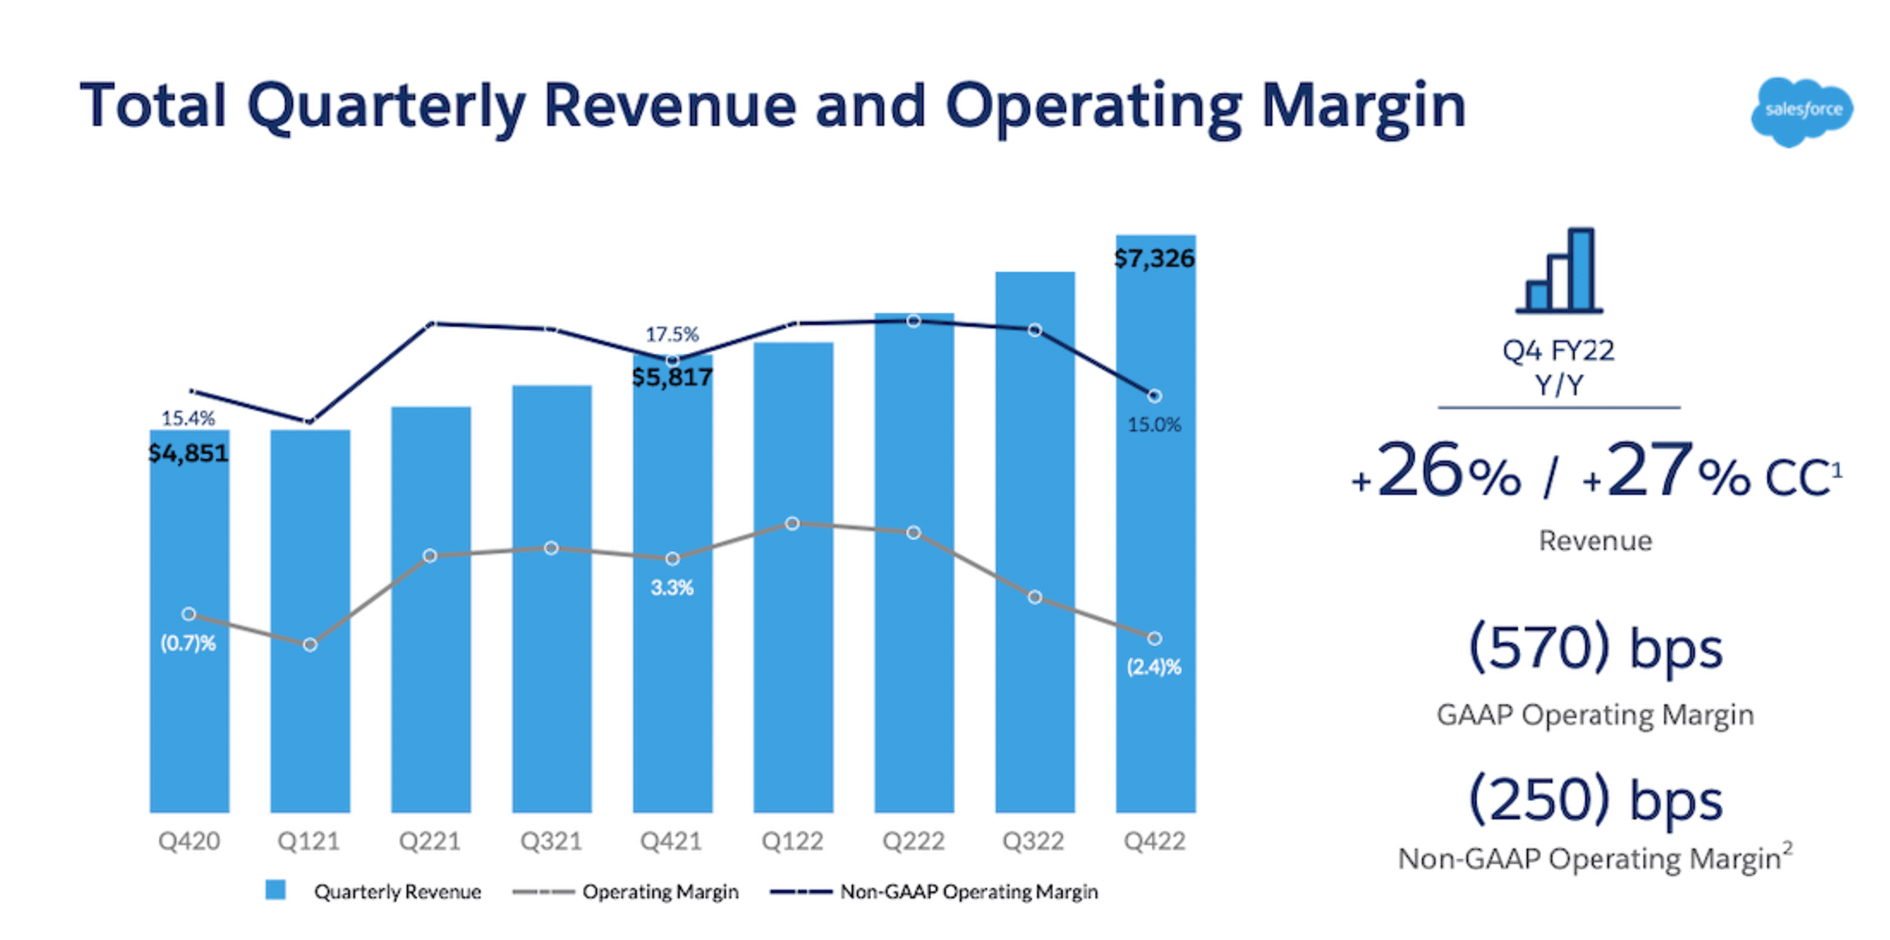
\includegraphics[width=0.8\textwidth]{Chapter1_Introduction/Pictures/Saleforce_Quaterly_Revenue.png}}
    \caption{SAP S/4HANA and Salesforce Market Share and Revenue Growth}
    \label{fig:salesforce_revenue}
\end{figure}


\subsection{Cost Efficiency and Performance Gains}
Organizations that have adopted SAP S/4HANA report substantial cost savings and operational improvements:
\begin{itemize}
    \item Fjellsport reduced inventory costs by 20\% through SAP S/4HANA’s real-time analytics \cite{sap_2025}.
    \item ENEL improved its billing efficiency by 50\%, enhancing cash flow management \cite{sap_2025}.
    \item Swiss Port Ltd lowered its TCO by 30\%, demonstrating the cost-effectiveness of SAP S/4HANA \cite{sap_2025}.
\end{itemize}

Similarly, Salesforce remains a high-ROI investment, with its Service Cloud alone generating \$8 billion in 2024, proving its financial sustainability and continued market growth \cite{statista_2023b}.


\subsection{Justification for This Research}

SAP S/4HANA is the largest and most dominant ERP system in the enterprise software market, trusted by the majority of Fortune 500 companies. Although SAP provides its own CRM solutions, adding SAP CRM to an existing SAP S/4HANA landscape represents a significant financial investment, making it impractical for many organizations. However, SAP's third-party CRM integration capabilities allow businesses to connect best-in-class solutions without committing to an entirely SAP-exclusive ecosystem.

Similarly, Salesforce stands as the largest CRM provider in the world, offering unparalleled CRM features. Salesforce natively supports third-party ERP integrations via APIs, allowing seamless DS between customer-facing processes and back-end ERP.

From a financial and operational standpoint, integrating SAP S/4HANA with Salesforce provides the best of both worlds leveraging SAP’s industry-leading ERP capabilities while taking advantage of Salesforce’s best-in-class CRM features. This integration ensures:
\begin{itemize}
    \item Cost-effectiveness, avoiding the high investment required for SAP's native CRM.
    \item Seamless interoperability, utilizing SAP’s support for third-party CRM solutions and Salesforce’s API-driven ERP integration.
    \item Optimized enterprise efficiency, combining the world’s most powerful ERP and CRM into a unified system.
\end{itemize}

Given that SAP is the undisputed leader in ERP solutions and Salesforce holds the largest market share in CRM, it makes both strategic and financial sense for businesses to integrate these two dominant systems. By doing so, organizations can maximize efficiency, reduce costs, and achieve seamless business operations without compromising on functionality.

This research will focus on how businesses can optimally integrate SAP S/4HANA and Salesforce, ensuring data consistency, automated workflows, and future proof system scalability. The findings will serve as a guide for companies looking to leverage this integration for financial and operational success.



%%%%%%%%%%%%%%%%%%%% Conclusion
\section{Conclusion}

The literature review in this thesis serves as the foundation for understanding the integration of SAP S/4HANA and Salesforce using SAP BTP Integration Suite. As enterprises increasingly rely on ERP and CRM systems to drive operational efficiency, the demand for seamless integration between these platforms has become paramount. However, achieving this integration is not without challenges, as evident from the extensive body of research analyzed in this chapter.

A key takeaway from the literature is the evolution of ERP and CRM systems. Initially, ERP was developed to centralize business processes, while CRM emerged as a specialized tool for managing customer interactions. Over the years, these systems have become indispensable, yet they largely function in silos. While SAP S/4HANA provides robust ERP capabilities, its CRM functionalities are limited compared to specialized platforms like Salesforce. This necessitates integration to ensure real-time DS, operational efficiency, and an enhanced customer experience.

One of the most pressing challenges in ERP-CRM integration is DS and consistency. Multiple studies indicate that data fragmentation occurs when ERP and CRM systems store information in separate databases, leading to discrepancies in customer records, order details, and sales forecasts. This fragmentation is exacerbated by differences in data structures, formats, and identifiers used in SAP S/4HANA and Salesforce. The literature highlights the need for middleware solutions to act as a bridge, ensuring seamless communication between these systems.

The second major challenge discussed is technical barriers, particularly API mismatches, security concerns, and performance limitations. SAP S/4HANA primarily relies on OData and SOAP-based web services, whereas Salesforce uses RESTful APIs and GraphQL, creating interoperability issues. Additionally, security concerns such as data protection, authentication, and encryption present obstacles to effective integration. Research has shown that enterprises must carefully design their integration architecture to balance security with real-time data access.

Given these challenges, middleware solutions have gained prominence as a viable approach to ERP-CRM integration. SAP BTP (BTP) Integration Suite has been identified as a leading middleware option, offering pre-built iFlows, API management, and monitoring tools. Unlike third-party solutions such as MuleSoft and Dell Boomi, SAP BTP provides native integration capabilities tailored for SAP environments. Its low-code/no-code interface, combined with pre-configured connectors for Salesforce, makes it an ideal choice for businesses leveraging both platforms.

A key contribution of this chapter is the assessment of SAP BTP's role in ERP-CRM integration. Studies indicate that SAP BTP excels in data transformation, real-time analytics, and compliance management. By providing built-in connectors for Salesforce and SAP S/4HANA, it reduces the complexity associated with custom integration efforts. Furthermore, its support for hybrid and multi-cloud architectures ensures flexibility for organizations operating in diverse IT landscapes.

Despite its advantages, SAP BTP is not without limitations. The literature review highlights research gaps, particularly the lack of practical implementation studies. While many studies discuss ERP-CRM integration in a theoretical or strategic context, few provide detailed technical guidance on configuring SAP BTP for SAP-Salesforce integration. This gap underscores the need for an implementation-focused study, which this thesis aims to address.

Another research gap identified is the lack of comparative analyses between SAP BTP and other middleware solutions specifically in the context of SAP S/4HANA and Salesforce integration. While this thesis does not focus on middleware comparisons, it acknowledges the potential benefits of evaluating how different middleware platforms handle data orchestration, security, and performance optimization.

Future trends in ERP-CRM integration, as explored in this chapter, suggest that AI-driven data mapping, serverless integration, and regulatory compliance will play an increasingly critical role. AI and ML can automate data transformation, reduce mapping errors, and optimize synchronization processes. Additionally, the rise of serverless middleware solutions presents new opportunities for scalable and cost-effective integrations.

From a compliance perspective, organizations must ensure GDPR, SOX, and industry-specific regulatory adherence when integrating ERP and CRM systems. The literature emphasizes that data protection mechanisms, audit trails, and access controls are crucial to preventing security breaches and maintaining trust in integrated environments.

The insights gathered from this literature review inform the direction of this thesis. Given the lack of practical implementation research, this study aims to provide a structured guide on integrating SAP S/4HANA and Salesforce using SAP BTP Integration Suite. By detailing the architecture, data mappings, API configurations, and real-world testing, this research will contribute a hands-on approach to middleware-based ERP-CRM integration.

Furthermore, this literature review lays the groundwork for the next chapter, which focuses on defining the business problem and case analysis. While this chapter provided a theoretical foundation, the next chapter will translate these insights into real-world business challenges, use cases, and justifications for implementing SAP BTP as the middleware of choice.

In conclusion, this literature review underscores the critical need for seamless ERP-CRM integration, the challenges associated with achieving it, and the role of middleware—specifically SAP BTP—in bridging the gap between SAP S/4HANA and Salesforce. While existing research highlights various strategies and potential solutions, it lacks a practical implementation guide, which this thesis seeks to provide. The findings of this chapter set the stage for a technical deep dive into SAP BTP’s capabilities and its application in a real-world business context.

%=== END OF CHAPTER TWO ===
\newpage



%=== CHAPTER THREE (3) ===
%=== (Actual work done and contribution, including literature survey) ===

\chapter{Business Problem \& Case Analysis}
\section{The Challenge of ERP-CRM Integration}

In today’s rapidly evolving business environment, organizations must operate efficiently while maintaining strong customer relationships. To achieve this, companies rely on ERP systems for internal operations and CRM systems for managing customer interactions. However, when these systems operate in isolation, businesses face operational inefficiencies, lack of real-time data visibility, and inconsistent customer experiences \cite{ruivo2014}. ERP-CRM integration is essential to unify these systems, ensuring a seamless flow of information across departments, improving decision-making, and enhancing customer satisfaction \cite{shaul2013}.

\subsection{Why ERP-CRM Integration is Necessary}

\subsubsection{Creating a Single Source of Truth}
ERP and CRM systems store vast amounts of customer, sales, financial, and operational data, but without integration, this information remains fragmented. When sales teams in a CRM system register customer details, but finance and operations in the ERP system do not have real-time access to this data, it creates inconsistencies and delays \cite{hendricks2007}. Integrating ERP and CRM ensures that all teams work with up-to-date and accurate data, reducing duplication and improving overall efficiency \cite{gebreyes2018}.

\subsubsection{Enhancing Customer Experience and Satisfaction}
Customers expect quick, personalized, and accurate service, whether they are interacting with sales, support, or finance. Without integration, customer service representatives may lack access to real-time order history, billing status, or past interactions, leading to slow and ineffective responses \cite{devarashetty2023}. By integrating ERP and CRM, companies can provide a 360-degree view of the customer, leading to faster resolutions, personalized recommendations, and higher customer loyalty \cite{mestre2015}.

\subsubsection{Improving Sales and Revenue Forecasting}
Sales and marketing teams rely on CRM data to analyze customer behavior, sales trends, and market demands, while ERP systems track inventory, production, and financial metrics. Without integration, sales teams may sell products that are out of stock, or finance teams may struggle with inaccurate revenue projections \cite{ruivo2014}. A fully integrated ERP-CRM system provides synchronized data, allowing businesses to make better forecasts, optimize inventory management, and reduce revenue losses \cite{shaul2013}.

\subsubsection{Reducing Operational Costs and Process Inefficiencies}
Managing separate ERP and CRM systems often leads to manual data entry, duplicate records, and miscommunications between departments. These inefficiencies result in higher labor costs, increased error rates, and time-consuming reconciliations \cite{hendricks2007}. By integrating both systems, businesses can automate workflows, reduce administrative burdens, and streamline operations, ultimately cutting costs and boosting productivity \cite{gebreyes2018}.

\subsubsection{Enhancing Compliance and Risk Management}
Many industries, such as finance, healthcare, and manufacturing, require strict compliance with regulatory standards like GDPR, SOX, and HIPAA. A lack of integration between ERP and CRM can make it difficult to maintain audit trails, enforce data security policies, and track transactions across systems \cite{devarashetty2023}. Integration enables companies to centralize compliance data, automate reporting, and ensure regulatory adherence, reducing legal risks and penalties \cite{ruivo2014}.

\paragraph{}
ERP-CRM integration is no longer optional but a strategic necessity for organizations seeking operational efficiency, improved customer experiences, and data-driven decision-making. However, businesses must navigate significant challenges, including technological limitations, organizational resistance, cost constraints, security risks, and data governance issues. Overcoming these hurdles requires a well-defined integration strategy, strong leadership, and investment in scalable middleware solutions. A fundamental obstacle that arises during ERP-CRM integration is \textbf{data fragmentation}. As organizations attempt to synchronize data across systems, they often encounter inconsistencies, redundancy, and delays. The next section delves into the concept of data fragmentation, its impact on business operations, and potential strategies to address these issues.

\section{Manual vs. Automated Data Transfer in ERP-CRM Systems}

In modern enterprise environments, the integration of disparate systems such as ERP and CRM has become a critical focus. One of the primary challenges organizations face is managing data transfer between these systems. Specifically, the choice between manual and automated transfer processes significantly impacts efficiency, accuracy, and scalability. This section explores these two approaches, highlighting their benefits and limitations within the context of ERP-CRM integration.

\subsection{Manual Data Transfer}

Traditionally, many organizations relied on manual processes to transfer data between systems. In this scenario, employees manually enter or transfer data from one system to another. For example, customer orders processed in a CRM system would need to be manually entered into the ERP system for fulfillment and invoicing. While this approach may seem manageable in small-scale operations, it becomes problematic as the organization grows.

Manual data entry increases the likelihood of human error, especially when dealing with large volumes of transactions. As one study notes, when ERP systems are used in isolation without CRM integration, "it is hard to have a comprehensive and real-time response for customers' needs" (Jiang, n.d.). This lack of integration causes delays and inaccuracies in data processing, as information is not synchronized across systems. Furthermore, operating systems independently often leads to data redundancy and discrepancies (Tomić \& Jovanović, 2016).

In addition to the risk of errors, manual processes are time-consuming. Data must be manually input, checked, and rechecked to ensure consistency. In a fast-paced business environment, this inefficiency diverts employees' time from higher-value activities, such as strategic planning and customer engagement.

\subsection{Automated Data Transfer}

In contrast, automated data transfer eliminates the need for manual intervention by using software to transfer data between systems without human involvement. Automation offers clear advantages in terms of speed, accuracy, and efficiency. As noted in the literature, "ERP takes a customer order and provides a software roadmap for automating the different steps along the path to fulfilling it. This eliminates manual intervention and reduces errors associated with human handling" (Al-Mudimigh, Saleem, \& Ullah, 2009). By automating workflows, organizations can ensure accurate, real-time data transfer, reducing processing time and discrepancies.

An integrated approach—where ERP and CRM systems communicate seamlessly—removes data silos that often result from manual data entry. "The integration of business processes, particularly in CRM and ERP systems, enhances the synchronization of business data across departments and improves decision-making" (Liu \& Jiang, n.d.). For example, when a customer places an order, automated systems can immediately push that data to the ERP system for fulfillment, eliminating the need for manual entry. This real-time data synchronization enhances operational efficiency and ensures decision-makers have access to the most current information.

The benefits of automation extend beyond speed and accuracy. As research highlights, "Automating integration processes... reduces the likelihood of errors and enhances the speed of processing transactions" (SAP, 2020). Additionally, automation frees employees from routine tasks, allowing them to focus on value-added activities, such as customer service and process optimization.

\subsection{Challenges of Manual Data Transfer}

Despite its apparent simplicity, manual data transfer has significant drawbacks. As mentioned earlier, manual processes are prone to errors and data inconsistencies, which can undermine business operations. These errors can lead to miscommunication, delays in service delivery, and, in some cases, financial losses due to incorrect billing or inventory discrepancies.

Moreover, manual processes are inherently slow and inefficient, often requiring extensive effort to reconcile data between systems. For larger organizations with vast amounts of data, this inefficiency becomes even more pronounced, as the time spent on manual tasks increases exponentially with scale.

\subsection{Advantages of Automated Transfer}

Automated data transfer offers several key advantages that make it the preferred choice for businesses aiming to optimize their operations:

\begin{itemize}
    \item \textbf{Efficiency}: Automated systems can handle large volumes of data in a fraction of the time required for manual processing.
    \item \textbf{Accuracy}: Automation reduces the likelihood of human error, ensuring consistent and error-free data transfer.
    \item \textbf{Cost-Effectiveness}: While the initial setup for automated systems may require investment, long-term savings come from reduced labor costs and fewer errors requiring remediation.
    \item \textbf{Scalability}: Automated processes can easily scale to handle increased data volumes as businesses grow, without the need for additional manual labor or system restructuring.
\end{itemize}

In conclusion, while manual data transfer may still be viable for small-scale operations, it poses significant challenges for larger, more complex businesses. The risks of errors, inefficiencies, and data inconsistencies associated with manual processes can undermine business performance and hinder growth. Automated data transfer, on the other hand, offers a scalable, efficient, and accurate solution to integration challenges. By adopting automated systems, businesses can streamline operations, enhance customer service, and reduce operational costs, positioning themselves for greater success in an increasingly competitive marketplace.

\section{Key Integration Issues and Their Business Impact}

\subsection{Business Challenges in ERP-CRM Integration}

\subsubsection{Technology and Infrastructure Compatibility}
ERP and CRM solutions often come from different vendors and may not be designed to work together out of the box. Legacy ERP systems, in particular, lack modern API capabilities, requiring additional customization or middleware solutions to enable integration \cite{shaul2013}. Businesses must evaluate their technology infrastructure and invest in scalable integration solutions to ensure seamless data exchange \cite{hendricks2007}.

\subsubsection{Resistance to Change and Organizational Alignment}
Integrating ERP and CRM involves changes in workflows, data management practices, and employee responsibilities. Many organizations face resistance from employees who are accustomed to existing processes or departments that prefer working in silos \cite{gebreyes2018}. Successful integration requires clear communication, training programs, and strong leadership support to drive adoption and ensure alignment across teams \cite{ruivo2014}.

\subsubsection{Implementation Costs and Complexity}
ERP-CRM integration projects require significant investment in software, middleware, IT resources, and ongoing maintenance. Companies often underestimate the complexity of integration, leading to budget overruns, extended timelines, and implementation failures \cite{mestre2015}. To mitigate these risks, organizations should develop a clear integration roadmap, assess ROI, and prioritize phased deployments to minimize disruption \cite{hendricks2007}.

\subsubsection{Security and Data Privacy Concerns}
As ERP and CRM systems store sensitive customer and financial data, integration increases exposure to cybersecurity risks, unauthorized access, and potential data breaches \cite{devarashetty2023}. Organizations must implement robust security measures, encryption protocols, and role-based access controls to safeguard critical business information \cite{ruivo2014}.

\subsubsection{Ensuring Data Accuracy and Governance}
One of the most significant challenges in ERP-CRM integration is maintaining consistent, high-quality data across both platforms. Mismatched data formats, duplicate customer records, and outdated information can lead to operational disruptions, reporting errors, and compliance violations \cite{gebreyes2018}. Establishing data governance policies, automated validation rules, and periodic audits is essential to maintaining data integrity and maximizing the value of integration \cite{shaul2013}.

\section{Key Integration Issues}

Enterprise systems such as SAP S/4HANA and Salesforce play a crucial role in modern businesses, enabling organizations to manage customer relationships (CRM) and ERP in an integrated manner. However, integrating these platforms presents significant challenges, particularly regarding APIs, data mapping, and security. These challenges must be addressed to ensure efficient business processes, data consistency, and secure transactions.

A robust integration framework must address three primary concerns:
\begin{itemize}
    \item APIs and system interoperability challenges, which affect how data is exchanged between SAP and Salesforce.
    \item Data mapping and transformation issues, which impact how different data formats, identifiers, and structures are aligned across systems.
    \item Security concerns, which involve ensuring that data remains protected, confidential, and compliant with regulatory requirements.
\end{itemize}

Each of these concerns is discussed in detail in the following subsections, starting with API integration challenges.

\subsection{API Integration Challenges}
API-based integration is the backbone of SAP S/4HANA and Salesforce interoperability, enabling automated data transfer, system synchronization, and business process execution. However, integrating two fundamentally different platforms introduces a range of technical challenges that organizations must address.

\subsubsection{Differences in API Architectures}
One of the most significant challenges in API integration is the inherent differences in architecture between SAP S/4HANA and Salesforce. SAP S/4HANA uses OData services and SOAP-based web services for data exchange, while Salesforce primarily supports REST APIs and GraphQL \cite{chinta2024}.

These differences create compatibility issues that require custom API connectors and middleware to enable efficient data flow between the two systems. Middleware platforms such as SAP Integration Suite or MuleSoft play a crucial role in bridging these gaps \cite{chinta2024}.

\subsubsection{Real-Time vs. Batch Processing}
Another critical API challenge is determining whether real-time or batch processing should be used for different types of data. Real-time integration is crucial for customer updates, order processing, and lead management, whereas batch processing is more efficient for large-volume financial transactions and historical data imports \cite{almudimigh2009}.

\subsubsection{Middleware and iPaaS Solutions for API Management}
Given the complexity of API-based integrations, businesses often rely on middleware solutions or Integration PaaS (iPaaS) platforms to manage, orchestrate, and monitor API calls \cite{chinta2024}. Middleware such as SAP BTP Integration Suite, MuleSoft, or Dell Boomi offers the following benefits:
\begin{itemize}
    \item Data transformation to convert SOAP/XML data from SAP into REST/JSON formats for Salesforce.
    \item Error handling mechanisms to retry failed API calls and log errors for debugging.
    \item Scalability and performance monitoring, ensuring optimized API requests even under high loads.
\end{itemize}

\subsubsection{Error Handling and Logging in API Calls}
API communication between SAP and Salesforce is prone to timeouts, authentication failures, and data transformation errors. According to \cite{chinta2024}, a robust error-handling mechanism must be in place to:
\begin{enumerate}
    \item Automatically retry failed API calls.
    \item Log API errors and trigger alerts for IT teams.
    \item Use queue-based processing for critical transactions such as financial updates and customer modifications.
\end{enumerate}

\subsubsection{API Authentication and Security Considerations}
Security is another major concern in API-based integrations. Unauthorized access to APIs can expose sensitive customer and financial data, leading to compliance violations and data breaches \cite{chinta2024}.

Security measures include:
\begin{itemize}
    \item OAuth 2.0 and JWT authentication for secure API access.
    \item IP Whitelisting to restrict API access to approved IP addresses only.
    \item Encryption in transit using TLS 1.2 or higher.
    \item API Gateway Monitoring to detect anomalies and prevent DDoS attacks.
\end{itemize}

\subsubsection{Custom API Connectors for Specialized Use Cases}
While SAP and Salesforce provide standard APIs, organizations often require custom API connectors to address unique business needs. For example, updating sales orders in SAP when Salesforce accounts are modified \cite{aljawarneh2018}.

\paragraph{}
API-based integration between SAP S/4HANA and Salesforce requires robust middleware, error-handling mechanisms, API security controls, and data transformation capabilities. Organizations must adopt a structured API integration strategy by leveraging iPaaS solutions, custom connectors, and hybrid real-time/batch processing models to achieve seamless data exchange.

\subsection{Data Mapping Challenges}
One of the fundamental challenges in integrating ERP and CRM systems is the disparity in data structures and mapping requirements. Data mapping plays a crucial role in ensuring that information flows seamlessly between systems, yet it is often hindered by differences in data storage, business logic, and identifier management.

\subsection{Structural Differences in Data Models}
ERP and CRM systems are designed for different purposes, leading to significant variations in data structures. ERP systems primarily focus on transactional processes, such as inventory management, procurement, and financial accounting, whereas CRM systems prioritize customer interactions, sales automation, and service tracking \cite{yanjing2009}.

For instance:
\begin{itemize}
    \item \textbf{ERP Systems:} Typically store customer data in financial and operational records categorized under accounts, invoices, and orders.
    \item \textbf{CRM Systems:} Maintain customer profiles, communication histories, and marketing campaigns that are often unstructured or semi-structured.
    \item \textbf{Issue:} Mapping customer data between these two systems can be complex because fields, attributes, and relationships may not align directly.
\end{itemize}

\subsection{Separate Databases and Identifier Conflicts}
Many organizations implement ERP and CRM systems separately, often from different vendors, leading to disparate database architectures. Even when both systems are from the same vendor, they often maintain separate data silos with unique identifiers for entities like customers, products, and transactions \cite{tomic2016}.

\subsection{Problems Arising from Separate Databases}
\begin{itemize}
    \item \textbf{Conflicting Unique Identifiers:} A customer may have different IDs in ERP and CRM.
    \item \textbf{Data Redundancy \& Inconsistency:} Customer records might exist in both systems but differ in details.
    \item \textbf{Multiple Sources of Truth:} Orders, invoices, and sales records might be updated in one system but not reflected in the other.
\end{itemize}

\subsubsection{Solution Approaches}
\begin{itemize}
    \item \textbf{Implement a Master Data Management (MDM) System:} Establishes a single version of truth for customer records across ERP and CRM.
    \item \textbf{Use Middleware for Real-Time Synchronization:} Ensures automated data reconciliation \cite{chinta2024}.
\end{itemize}

\subsection{Inconsistent Business Logic and Workflow Mapping}
ERP and CRM systems follow different business processes, leading to workflow mismatches during integration.

\subsubsection{Examples of Workflow Mismatches}
\begin{itemize}
    \item \textbf{Sales Order Processing:} ERP requires complex approval processes, whereas CRM enables quick deal closures.
    \item \textbf{Product Catalog \& Pricing Discrepancies:} ERP and CRM may store product pricing differently, causing inconsistencies in invoice generation.
\end{itemize}

\subsubsection{Solution Approaches}
\begin{itemize}
    \item \textbf{Business Process Alignment:} Define a unified workflow ensuring that ERP and CRM follow a consistent order management cycle.
    \item \textbf{Data Transformation \& Mapping Tools:} Use integration adapters that convert CRM sales order formats into ERP-compatible records.
\end{itemize}

\subsection{Challenges in Data Format and Field Mapping}
Different ERP and CRM solutions store data in varied formats:
\begin{itemize}
    \item ERP often uses structured, relational databases with strict field definitions.
    \item CRM allows for flexible, non-standardized customer data fields \cite{tomic2016}.
\end{itemize}

\subsubsection{Common Field Mapping Issues}
\begin{center}
    \begin{table}[h]
        \centering

        \begin{tabular}{|c|c|c|c|}
            \hline
            \textbf{Data Type} & \textbf{ERP Format} & \textbf{CRM Format} & \textbf{Integration Problem} \\
            \hline
            Customer Name & Last, First & Full Name & Split/Merge needed \\
            \hline
            Date Fields & YYYY-MM-DD & MM/DD/YYYY & Format mismatch \\
            \hline
            Address Fields & Street, City, ZIP & Combined Address & Requires Parsing \\
            \hline
            Product Codes & Numeric SKU & Text-Based SKU & Needs conversion \\
            \hline
        \end{tabular}
        \label{tab:field_mapping_issues}
        \caption{Common Field Mapping Issues Between ERP and CRM Systems}
    \end{table}
\end{center}

\subsubsection{Solution Approaches}
\begin{itemize}
    \item \textbf{Data Transformation Layers:} Middleware tools help convert data formats during transfer.
    \item \textbf{Pre-Migration Data Cleanup:} Standardizing field formats before integration prevents errors.
\end{itemize}

\paragraph{}
Data mapping remains one of the most critical and complex aspects of ERP-CRM integration. Organizations must adopt a combination of data governance policies, middleware solutions, and real-time synchronization mechanisms to ensure consistent, reliable, and high-quality data integration.

\section{Expected Benefits of SAP BTP Integration}

SAP BTP (Business Technology Platform) Integration Suite provides a robust cloud-based solution that streamlines business processes by enabling seamless integration of SAP and non-SAP applications. The suite offers multiple benefits that enhance operational efficiency, improve data management, and foster business agility. Below are some of the key advantages:

\subsection{Improved Productivity}
By automating data exchanges and integration processes between SAP S/4HANA and Salesforce, SAP BTP Integration Suite eliminates the need for manual data entry and process management. This results in increased operational efficiency and time savings, allowing businesses to focus on core activities rather than repetitive data-handling tasks \cite{bagga2023practical}.

\subsection{Enhanced Data Accuracy}
Integrating SAP S/4HANA with Salesforce through the SAP Integration Suite ensures data consistency and reliability across multiple systems. The real-time synchronization of business partner data prevents discrepancies that often arise from siloed information, thus improving decision-making and reporting accuracy \cite{bagga2023introduction}.

\subsection{Better Customer Service}
The integration enables a unified view of customer data by connecting SAP S/4HANA with CRM systems such as Salesforce. This allows organizations to provide faster, more accurate responses to customer inquiries, leading to enhanced customer satisfaction and loyalty \cite{bagga2023introduction}.

\subsection{Increased Business Agility \& Flexibility}
SAP BTP Integration Suite enables businesses to quickly adapt to changing market demands and operational requirements. With pre-built connectors, API management tools, and low-code development features, organizations can modify integration flows without extensive coding efforts. This flexibility reduces downtime and accelerates the deployment of new business processes \cite{bagga2023practical}.

\subsection{Cost Savings through Automation}
By replacing manual data entry and disconnected workflows with automated integration scenarios, businesses can significantly reduce labor costs and minimize errors. The automation of key business processes results in long-term cost savings and an improved return on investment (ROI) \cite{bagga2023introduction}.

\subsection{Support for Hybrid \& Multi-Cloud Environments}
SAP Integration Suite supports hybrid integration scenarios, enabling businesses to connect on-premise SAP S/4HANA systems with cloud-based solutions like Salesforce. This ensures that enterprises can leverage both legacy infrastructure and modern cloud applications without disrupting existing workflows \cite{bagga2023practical}.

\subsection{Scalability \& Future-Proofing}
SAP BTP Integration Suite is designed to scale with business growth. Whether a company expands its operations, adopts new applications, or integrates additional business units, the platform provides the necessary flexibility to accommodate evolving business needs \cite{bagga2023practical}.

\subsection{Secure \& Compliant Data Transfers}
Security is a critical factor in integration, and SAP BTP Integration Suite includes robust security measures such as encryption, authentication mechanisms, and compliance with data protection regulations. This ensures that sensitive business and customer data remains protected during integrations \cite{bagga2023practical}.

\paragraph{}
SAP BTP Integration Suite offers a comprehensive and future-ready middleware for organizations looking to integrate SAP S/4HANA with Salesforce and other enterprise applications. By enhancing efficiency, agility, and security, businesses can leverage seamless integrations to drive digital transformation and optimize operations. The suite’s low-code capabilities, pre-built integration packages, and real-time data synchronization make it a valuable asset for organizations aiming to maximize the potential of their ERP and CRM systems.

%=== END OF CHAPTER THREE ===
\newpage
%=== CHAPTER FOUR (4) ===
%=== Test and Experiments ===

\chapter{Technical Implementation \& Solution}
\section{Architecture Overview}

Integrating SAP S/4HANA with Salesforce using the SAP Business Technology Platform (BTP) Integration Suite enables seamless DS betweenERP andCRM systems. This integration facilitates real-time data exchange, streamlines business processes, and enhances operational efficiency.

SAP S/4HANA is anERP business suite built on the SAP HANA in-memory database platform. It is an on-premise system designed to facilitate the management of diverse business processes within an organization. On the other hand, Salesforce is a cloud-based software-as-a-service (SaaS) platform specializing inCRM, offering tools to automate sales and marketing processes for enterprises.

The integration framework within SAP Cloud Integration for SAP S/4HANA and Salesforce enables the synchronization of master data, including product, customer, and pricing information. This integration framework supports the automation of business processes by connecting SAP S/4HANA with Salesforce through the SAP Cloud Platform Integration (CPI). Data is extracted from SAP S/4HANA using the OData adapter, which is then mapped and transformed into a structure compatible with Salesforce SObjects. Subsequently, the transformed data is transmitted to Salesforce via the Salesforce Adapter. In scenarios where data flows from Salesforce to SAP S/4HANA, the information is similarly transformed and mapped within SAP CPI before being sent to SAP S/4HANA using the OData adapter. This bidirectional integration ensures seamless data exchange and process automation between the two systems.


\begin{figure}[H]
    \centering
    \fbox{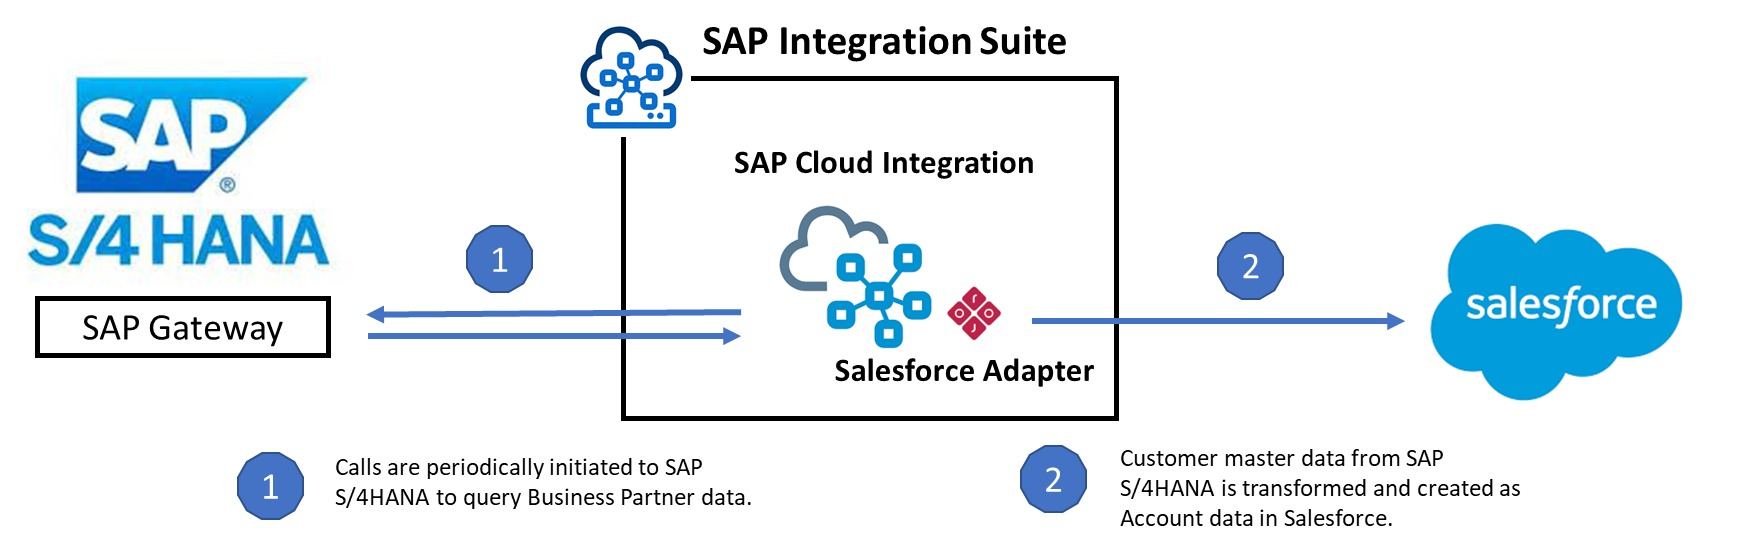
\includegraphics[width=0.8\textwidth]{Chapter4/Pictures/Arct_ov.jpg}}
    \caption{Overview of System Architecture}
    \label{fig:impl}
\end{figure}

\subsection{Prerequisites}

To successfully configure the integration content as described in this guide, it is imperative to ensure that you have the necessary access rights and authorizations for the systems involved. This configuration is pivotal for establishing a robust integration between SAP S/4HANA and Salesforce, leveraging BTP Middleware, specifically SAP Cloud Platform Integration (CPI). Below is a detailed breakdown of the access and authorization requirements for each system.

\subsubsection{Access Requirements}
\begin{itemize}
    \item \textbf{SAP S/4HANA Tenant Details:}
    \begin{itemize}
        \item You must have access to the SAP S/4HANA system, which serves as the core ERP platform for managing business processes.
        \item Ensure connectivity to the SAP S/4HANA tenant, as it will act as the source or target system for data exchange during the integration process.
    \end{itemize}

        \begin{figure}[H]
    \centering
    \fbox{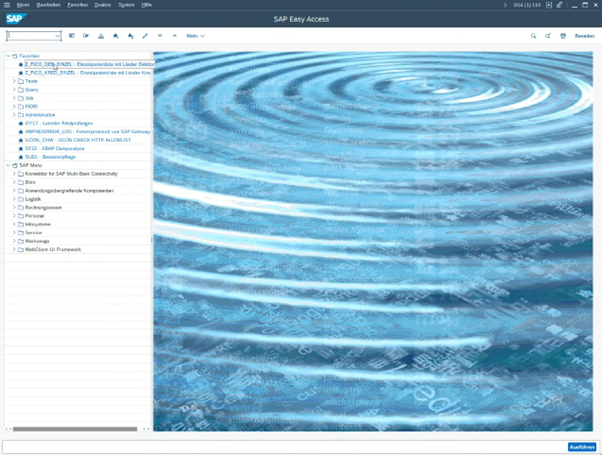
\includegraphics[width=0.8\textwidth]{Chapter4/Pictures/s4hana.png}}
    \caption{S4 Hana Home Page}
    
\end{figure}

    \item \textbf{SAP Cloud Platform Integration (CPI) Tenant Details:}
    \begin{itemize}
        \item Access to the SAP CPI tenant is required, as it functions as the middleware facilitating the integration between SAP S/4HANA and Salesforce.
        \item The CPI tenant will host the integration flows, mappings, and transformations necessary for seamless DS.
    \end{itemize}

\begin{figure}[H]
    \centering
    \fbox{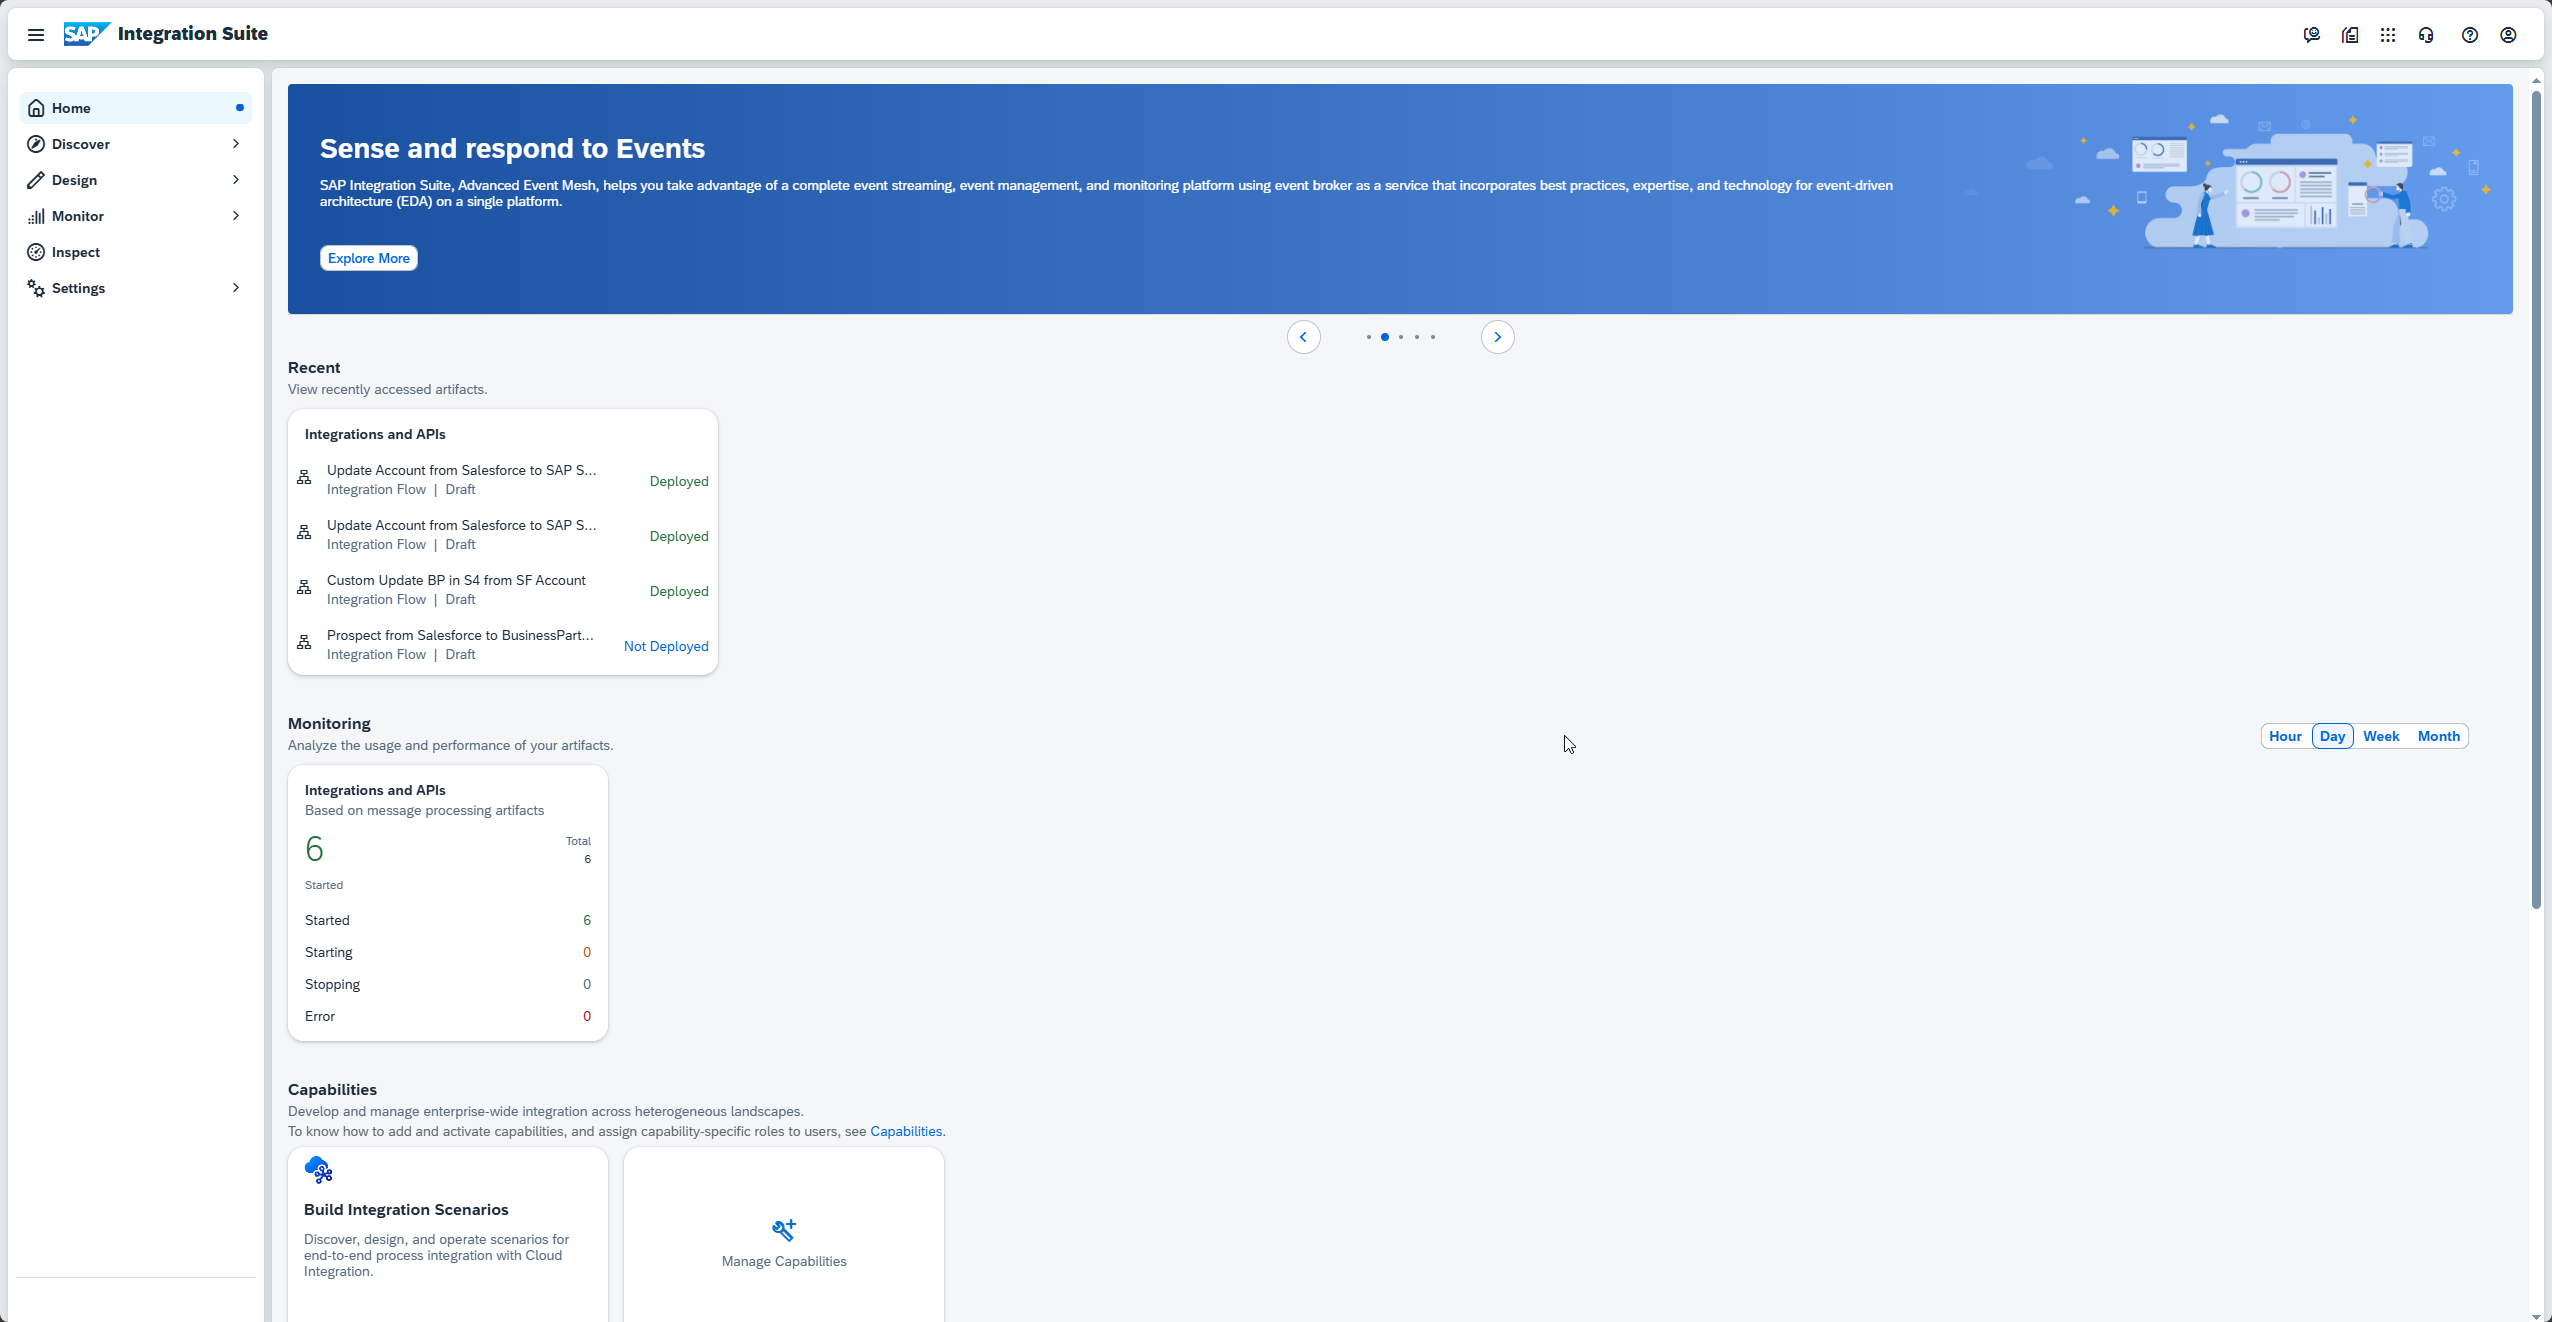
\includegraphics[width=0.8\textwidth]{Chapter4/Pictures/integrationsuite.png}}
    \caption{Integration Suite Home Page}
    
\end{figure}
    

    \item \textbf{Salesforce Tenant Details:}
    \begin{itemize}
        \item Access to the Salesforce tenant is essential, as it serves as the CRM platform where customer, product, and sales-related data will be synchronized.
        \item Ensure connectivity to the Salesforce environment to enable bidirectional data exchange with SAP S/4HANA.
    \end{itemize}
\end{itemize}


\begin{figure}[H]
    \centering
    \fbox{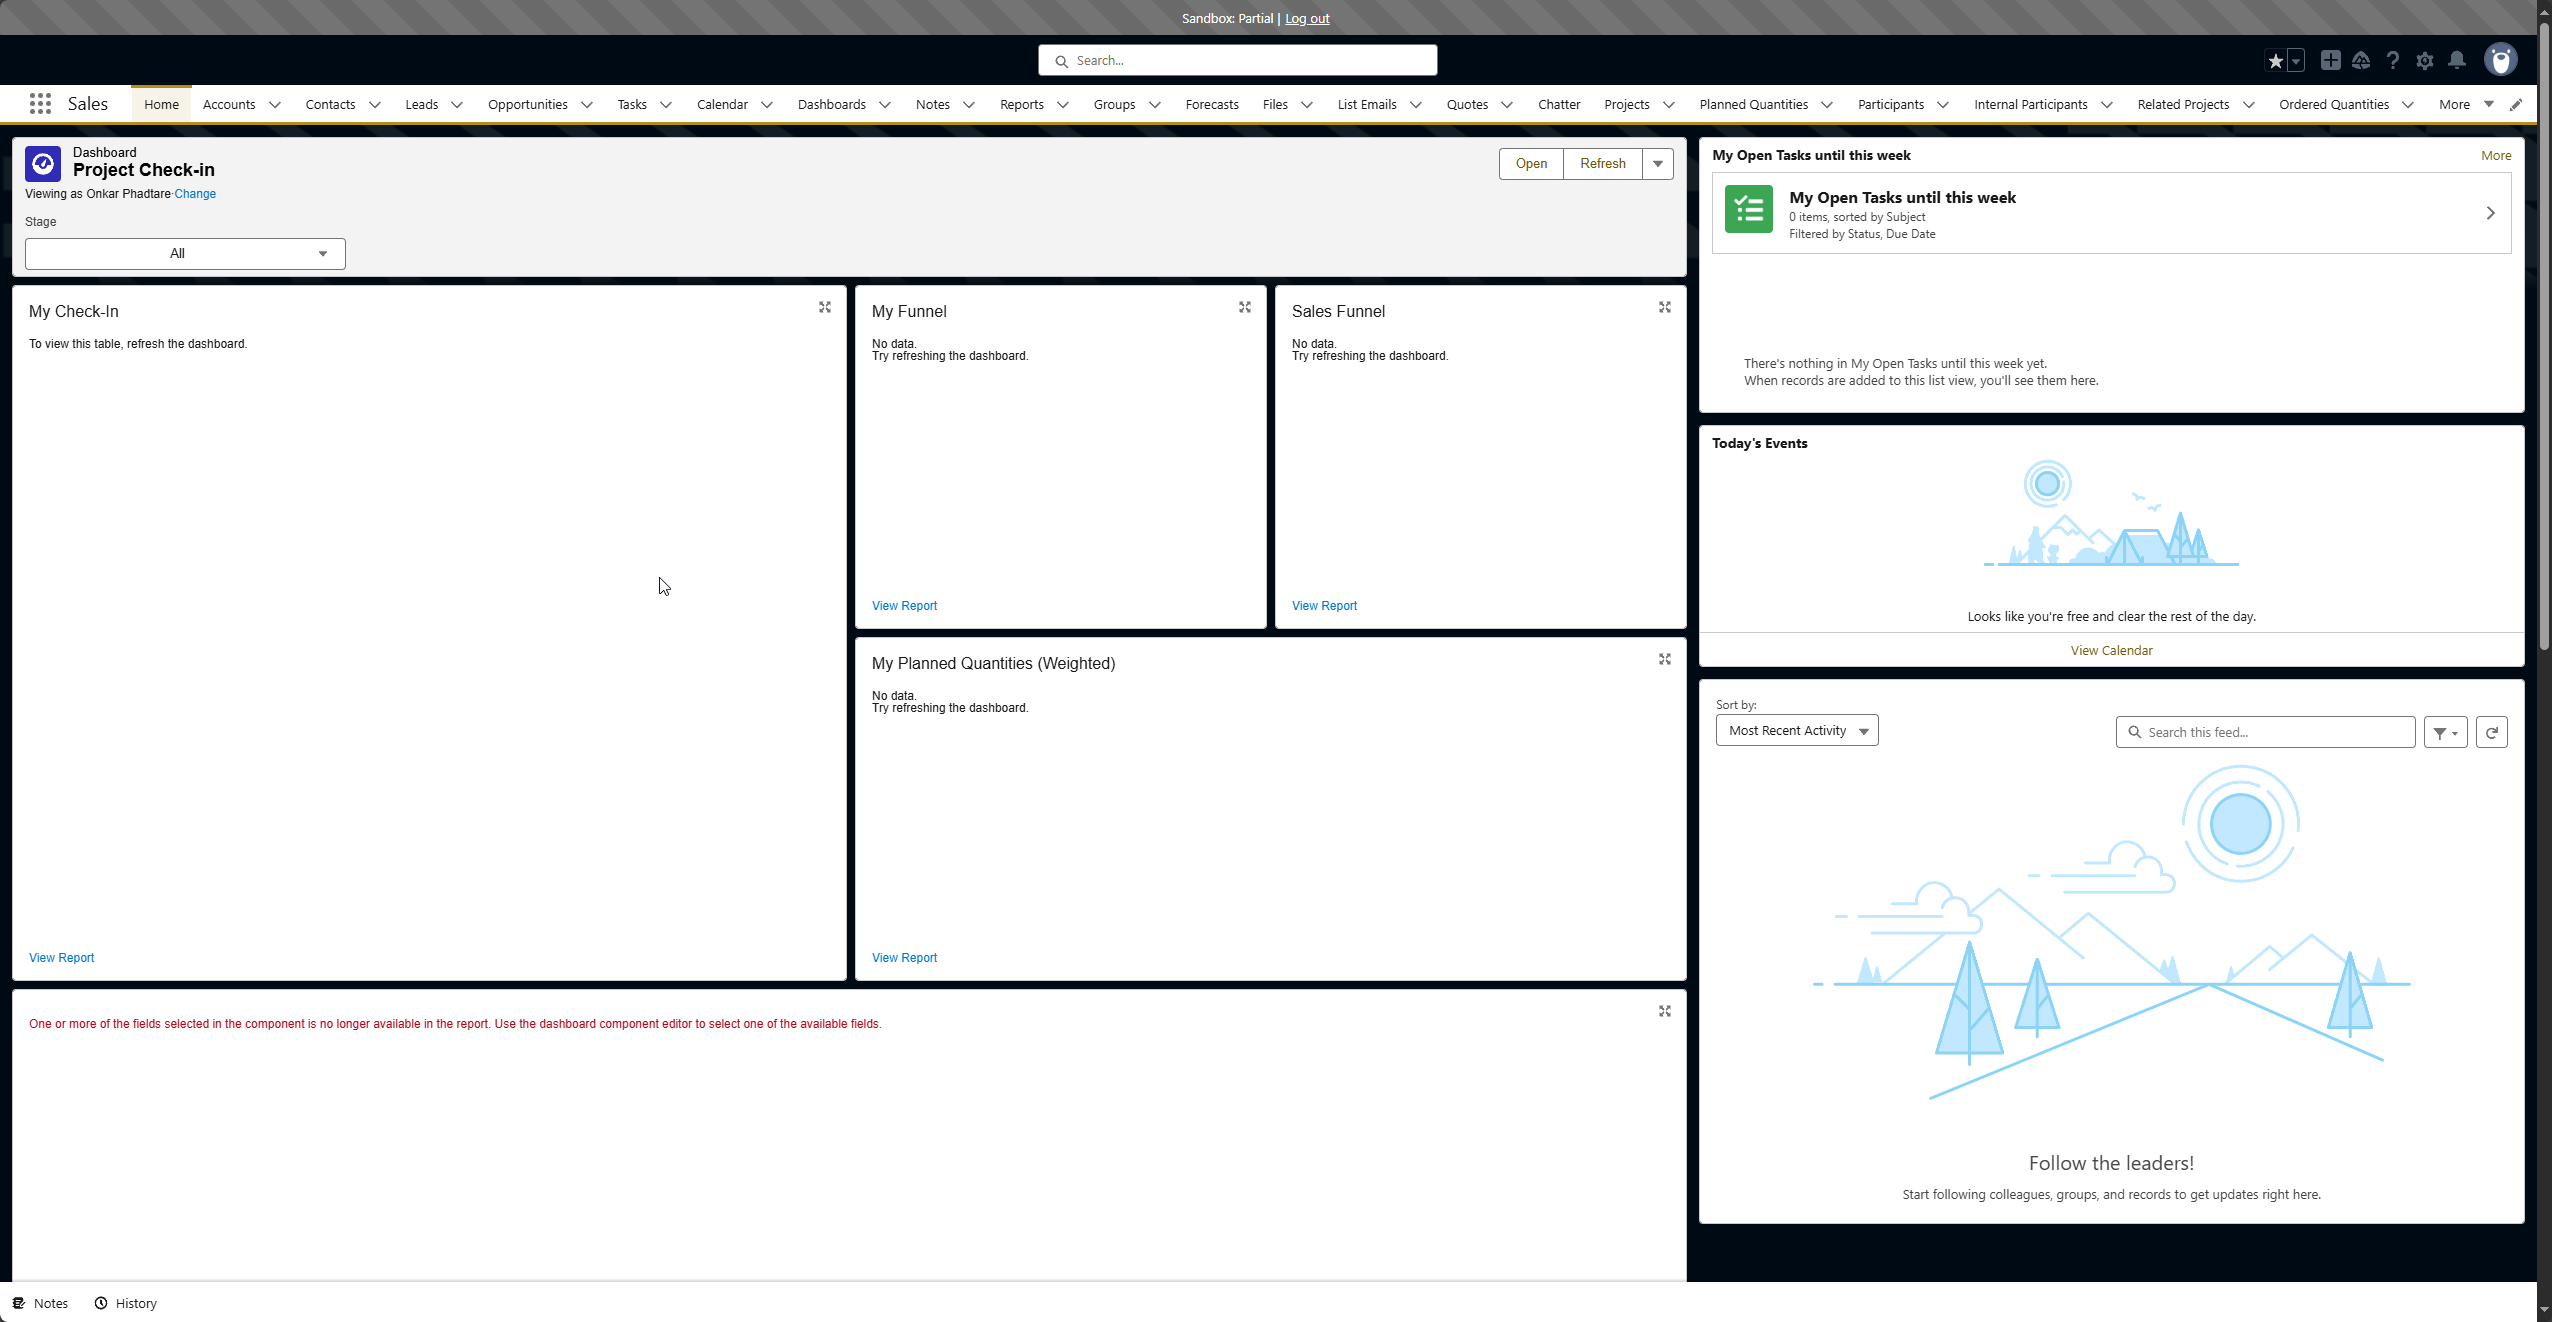
\includegraphics[width=0.8\textwidth]{Chapter4/Pictures/salesforce.png}}
    \caption{Salesforece Home Page}
    
\end{figure}

\subsubsection{Authorization Requirements}
\begin{itemize}
    \item \textbf{SAP S/4HANA Tenant Details:}
    \begin{itemize}
        \item \textbf{Access to SAP Gateway:} You must have permissions to access the SAP Gateway, which enables the exposure of OData services required for data extraction and integration.
        \item \textbf{User Creation and Role Assignment:} You need the ability to create users and assign appropriate roles within the SAP S/4HANA system to ensure secure and authorized access to data.
        \item \textbf{Access to Master Data (Product Master):} Permissions to access and manage Product Master data are necessary, as this data will be synchronized with Salesforce.
        \item \textbf{Access to Sales Master Data:} You must have access to Sales Master Data, which includes customer and pricing information, to facilitate accurate data exchange.
        \item \textbf{Access to Sales Order Data:} Permissions to access Sales Order data are required, as this information may need to be shared or updated between SAP S/4HANA and Salesforce.
    \end{itemize}

    

    \item \textbf{SAP Cloud Platform Integration (CPI) Tenant Details:}
    \begin{itemize}
        \item \textbf{Authorization Group (\texttt{AuthGroup.IntegrationDeveloper}):} You must be assigned the \texttt{AuthGroup.IntegrationDeveloper} role within SAP CPI to design, configure, and deploy integration flows. This role grants the necessary permissions to create and manage integration artifacts, such as mappings, transformations, and adapters.
    \end{itemize}

    \begin{figure}[H]
    \centering
    \fbox{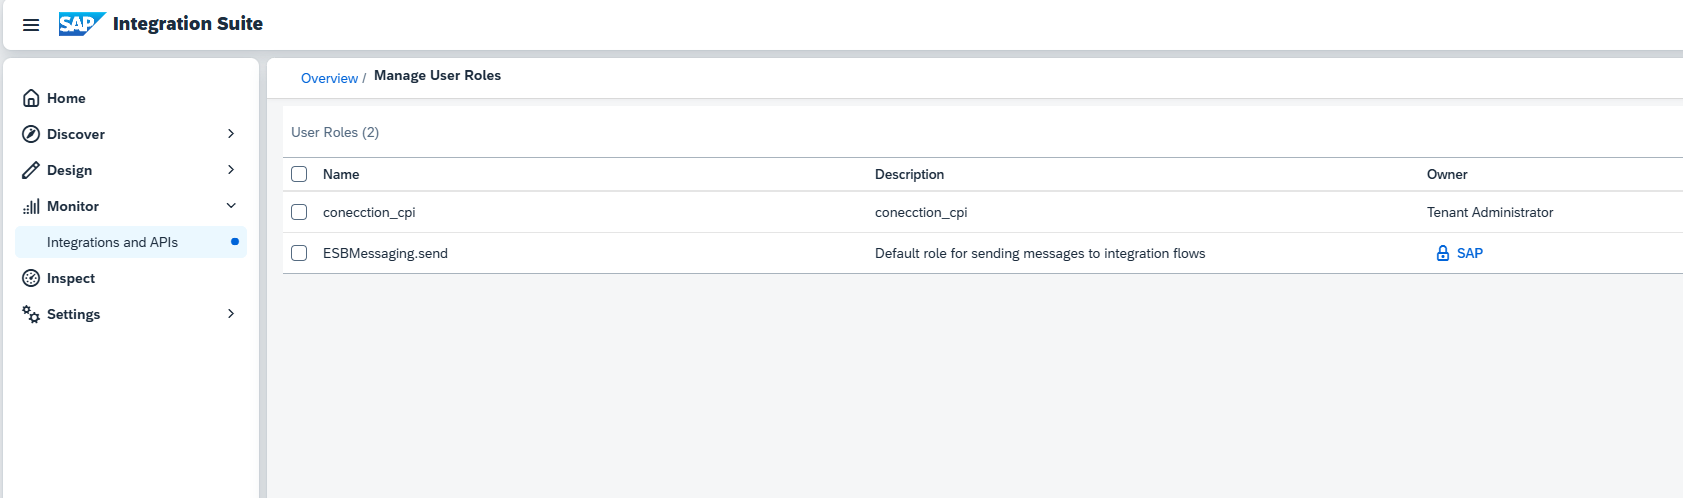
\includegraphics[width=0.8\textwidth]{Chapter4/Pictures/integrationrole.png}}
    \caption{SAP Cloud Platform Integration (CPI) Tenant Details:}
    
    \end{figure}

    \item \textbf{Salesforce Tenant:}
    \begin{itemize}
        \item \textbf{Appropriate Permissions for Configuration:} You must have sufficient permissions within the Salesforce tenant to configure and manage the integration. This includes the ability to create and modify Custom Fields for specific Salesforce objects (e.g., Account, Contact, Opportunity) that will be involved in the integration.
        \item \textbf{Access to Salesforce APIs:} Ensure that you have access to Salesforce APIs, as they will be used to send and retrieve data between Salesforce and SAP CPI.
        \item \textbf{Permission to Manage Integration User:} You may need to create or configure an integration user in Salesforce with the necessary permissions to allow data exchange with SAP CPI.
    \end{itemize}
\end{itemize}


The successful configuration and operation of the integration between SAP S/4HANA and Salesforce via SAP BTP Middleware (CPI) depend on fulfilling the access and authorization requirements outlined above. These prerequisites ensure that the integration flows can be designed, deployed, and executed seamlessly, enabling efficient DS and process automation across the two platforms. Proper configuration of both systems, along with the necessary permissions, is critical to achieving a robust and reliable integration solution.

\subsection{Adapter Installation }
The configuration of the Salesforce Adapter within the SAP Cloud Platform Integration (CPI) is a critical step in enabling seamless and secure data exchange between Salesforce and SAP S/4HANA. SAP CPI serves as an intermediary platform that facilitates the integration of business-critical data across these systems. To ensure secure and efficient communication, Salesforce employs an OAuth-based authentication mechanism, which provides a robust framework for secure API access. The configuration process involves two primary components: the installation of the Salesforce Adapter and the establishment of authentication mechanisms. Below is a detailed elaboration of these steps.

\begin{enumerate}
    \item \textbf{Installing the Salesforce Adapter} \\
    The Salesforce Adapter is a specialized integration component that enables connectivity between SAP CPI and Salesforce. Its installation is a prerequisite for creating integration flows that leverage Salesforce APIs. The installation process involves the following steps:
    \begin{itemize}
        \item Download the Salesforce Adapter package in .zip format from the appropriate source.
        \item Log into the SAP CPI Integration Suite and navigate to the \textit{Design} section, followed by \textit{Integration Suite}.
        \item Select the \textit{Edit} option and choose \textit{Add Integration Adapter} to initiate the installation process.
        \item Upload the downloaded Salesforce Adapter package in .zip format.
        \item Confirm the installation by clicking \textit{OK}.
        \item Navigate to \textit{Integration Monitor} and select \textit{Manage Integration Content} to verify the adapter's availability.
        \item Deploy the adapter to activate it for use in integration flows.
    \end{itemize}
    Upon successful deployment, the Salesforce Adapter becomes operational and can be utilized to design and execute integration flows between SAP CPI and Salesforce.

    \item \textbf{Establishing Authentication with Salesforce} \\
    To ensure the secure transfer of data, authentication credentials must be configured within SAP CPI. This involves setting up two distinct authentication mechanisms: Salesforce User Authentication and OAuth Authentication for the Salesforce Connected App. The steps for each are outlined below:
    \begin{itemize}
        \item \textbf{Salesforce User Authentication}:
        \begin{itemize}
            \item Navigate to the \textit{Security} section in SAP CPI and select \textit{Create Credentials}.
            \item Enter the following details:
            \begin{itemize}
                \item \textit{Username}: The email address associated with the Salesforce account.
                \item \textit{Password}: The password for the Salesforce account.
            \end{itemize}
            \item Click \textit{Deploy} to finalize the configuration.
        \end{itemize}
        \item \textbf{OAuth Authentication for Salesforce Connected App}:
        \begin{itemize}
            \item In Salesforce, create a \textit{Connected App} to generate OAuth credentials, including the \textit{Consumer Key}, \textit{Consumer Secret}, and \textit{Security Token}. The security token is typically sent to the registered email address.
            \item Copy the generated OAuth credentials from the Connected App.
            \item Return to SAP CPI and navigate to the \textit{Security} section, then select \textit{Create Credentials}.
            \item Configure the OAuth Client Credentials using the copied values from the Connected App.
            \item Deploy the credentials to establish a secure connection between SAP CPI and Salesforce.
        \end{itemize}
    \end{itemize}
    Once these authentication mechanisms are configured, SAP CPI can securely authenticate API requests to Salesforce, ensuring the protected exchange of business-critical data.
\end{enumerate}

In summary, the configuration of the Salesforce Adapter in SAP CPI involves a systematic approach to installing the adapter and establishing secure authentication mechanisms. This process ensures that the integration between Salesforce and SAP S/4HANA is both efficient and secure, enabling organizations to leverage their data effectively while maintaining compliance with security standards.


\section{Configuration}

Before the integration content package can be configured and deployed, it is essential to ensure that the respective systems SAP S/4HANA, Salesforce, and SAP Cloud Platform Integration (CPI) are properly configured and prepared. This preparatory phase involves establishing the necessary technical and operational prerequisites to facilitate seamless data exchange and process automation between the systems. The configuration process requires meticulous attention to system settings, access permissions, and connectivity parameters to ensure compatibility and functionality. Detailed steps for achieving this configuration are outlined in the subsequent sections of this guide. These steps provide a structured approach to preparing the systems, enabling the successful deployment and execution of the integration content package.

\subsection{Configuration in SAP S/4HANA }

This section outlines the essential configurations that must be executed within the SAP S/4HANA system as a prerequisite to initiating the implementation of Salesforce-related configurations or the setup of integration content in SAP Cloud Platform Integration (CPI). These mandatory configurations are critical to ensuring that the SAP S/4HANA system is fully prepared to support seamless data exchange and process integration with Salesforce and SAP CPI. The steps detailed in the subsequent sub-sections provide a systematic and comprehensive guide to completing these configurations, thereby establishing a robust foundation for the integration process. Adherence to these steps is imperative to achieve compatibility, functionality, and operational efficiency across the integrated systems.

\subsubsection{Create Technical Communication User }

A Technical Communication User is a prerequisite for enabling the invocation of OData services in SAP S/4HANA from SAP Cloud Platform Integration (CPI). This user serves as a dedicated entity for facilitating inbound communication and processing messages within the SAP S/4HANA system. The creation of such a user is a critical step in establishing secure and authorized communication between SAP S/4HANA and external systems, such as SAP CPI, during the integration process. Below is a detailed procedural guide for creating a communication user in SAP S/4HANA.

\paragraph{Procedure}
\begin{enumerate}
    \item \textbf{Access the Transaction Code:}
    \begin{itemize}
        \item Launch the SAP GUI and enter the transaction code \texttt{SU01} to access the User Maintenance interface.
    \end{itemize}

    \item \textbf{User Maintenance Initial Screen:}
    \begin{itemize}
        \item On the initial screen, input the desired \texttt{<User ID>} in the designated field. This ID will uniquely identify the technical communication user.
    \end{itemize}

    \item \textbf{Initiate User Creation:}
    \begin{itemize}
        \item Select the "Create" option to proceed with the creation of a new user.
    \end{itemize}

    \item \textbf{Maintain User Details:}
    \begin{itemize}
        \item Navigate to the "Maintain User" screen and populate the required fields with the following values:
        \begin{itemize}
            \item \textbf{Last Name:} Provide a descriptive name for the user.
            \item \textbf{Logon Data Tab:}
            \begin{itemize}
                \item Set the \textbf{User Type} to "Communication Data" to designate the user as a technical communication user.
                \item Assign a secure \texttt{<password>} to ensure authentication.
            \end{itemize}
        \end{itemize}
        \item \textbf{Note:} It is imperative to assign the user appropriate authorizations to enable the execution of OData API calls. These authorizations are essential for the user to interact with OData services effectively.
    \end{itemize}

    \item \textbf{Save the Configuration:}
    \begin{itemize}
        \item Once all fields have been populated, click the "Save" button to finalize the creation of the technical communication user.
    \end{itemize}
\end{enumerate}

The creation of a technical communication user is a foundational step in the integration process, as it ensures secure and authorized access to SAP S/4HANA's OData services. This user acts as a bridge between SAP S/4HANA and SAP CPI, enabling the seamless exchange of data and the execution of integration workflows. Proper configuration and authorization of this user are critical to maintaining system security, operational efficiency, and compliance with integration requirements.

    \begin{figure}[H]
    \centering
    \fbox{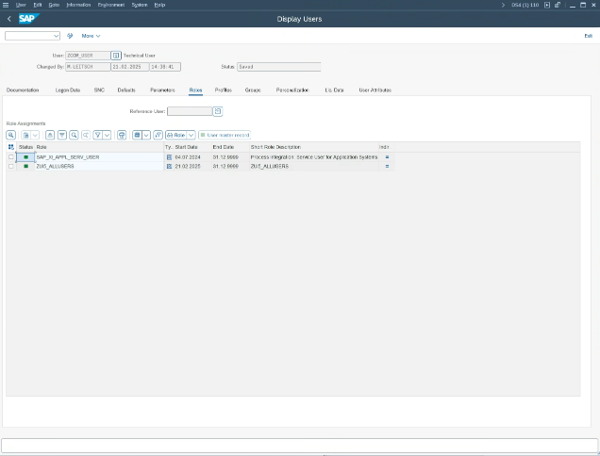
\includegraphics[width=0.8\textwidth]{Chapter4/Pictures/s4hana_role.png}}
    \caption{S4 HANA Communication user}
    
\end{figure}


\subsubsection{Activating SAP Gateway }

Before utilizing the SAP Gateway functionality, it is essential to ensure that it is globally activated within the SAP S/4HANA system. SAP Gateway serves as a critical component for enabling OData services, which facilitate communication between SAP S/4HANA and external systems, such as SAP Cloud Platform Integration (CPI). If SAP Gateway is not activated, OData services will not function, resulting in communication failures between consumer servers and the SAP system. In such cases, any system attempting to call these services will receive an error message. 

The activation process involves configuration activities that can be performed via the SAP Reference IMG (transaction code: \texttt{SPRO}). Specifically, the configuration settings are located under the path: \texttt{SAP NetWeaver > SAP Gateway > OData Channel > Configuration > User Settings and Connection Settings}. Once these configurations are completed, SAP Gateway must be activated using the steps outlined below.

\paragraph{Procedure}
\begin{enumerate}
    \item \textbf{Access the SAP Reference IMG:}
    \begin{itemize}
        \item Launch the SAP GUI and enter the transaction code \texttt{SPRO} to access the SAP Reference IMG.
    \end{itemize}

    \item \textbf{Navigate to SAP Gateway Configuration:}
    \begin{itemize}
        \item Within the SAP Reference IMG, navigate to the following path: \\
        \texttt{SAP NetWeaver > SAP Gateway > OData Channel > Configuration > Activate or Deactivate SAP Gateway}.
        \item Click on the "Activity" icon to proceed. A confirmation message will be displayed.
    \end{itemize}

    \item \textbf{Activate SAP Gateway:}
    \begin{itemize}
        \item Select the "Activate" option to enable SAP Gateway. Upon activation, a message will be displayed to confirm the current status of SAP Gateway.
    \end{itemize}
\end{enumerate}

The activation of SAP Gateway is a fundamental step in enabling OData services, which are essential for seamless communication between SAP S/4HANA and external systems. Without activation, OData services remain non-functional, leading to communication failures and disruptions in integration workflows. Proper activation ensures that consumer servers can interact with SAP S/4HANA effectively, facilitating data exchange and process automation. This step is critical for maintaining system functionality, operational efficiency, and compliance with integration requirements.


\subsubsection{Activate OData API in Gateway}
The integration between Salesforce and SAP S/4HANA relies on the OData APIs provided by SAP S/4HANA. These APIs serve as the foundation for enabling seamless data exchange and process automation between the two systems. To facilitate this integration, the relevant OData APIs must be activated in SAP Gateway. This section provides a detailed procedural guide for activating the OData APIs required by the integration content.

\paragraph{Procedure}
\begin{enumerate}
    \item \textbf{Access the Transaction Code:}
    \begin{itemize}
        \item Launch the SAP GUI and enter the transaction code \texttt{/IWFND/MAINT\_SERVICE}. This transaction displays the Service Catalog, which lists all activated Gateway services in the target system and allows for the addition of new services.
    \end{itemize}

    \item \textbf{Add a New Service:}
    \begin{itemize}
        \item Click the "Add Service" button located in the toolbar to initiate the process of adding a new service.
    \end{itemize}

    \item \textbf{Enter System Alias:}
    \begin{itemize}
        \item Input the System Alias of your front-end server in the designated field.
    \end{itemize}

    \item \textbf{Enter External Service Name:}
    \begin{itemize}
        \item Specify the External Service Name as \texttt{API\_BUSINESS\_PARTNER}.
    \end{itemize}

    \item \textbf{Retrieve Available Services:}
    \begin{itemize}
        \item Click the "Get Services" button in the toolbar to retrieve the list of available services. The requested service will be displayed for selection.
    \end{itemize}

    \item \textbf{Select and Add the Service:}
    \begin{itemize}
        \item Select the service generated from the previous step and click "Add Selected Services" or use the object link for further selection.
    \end{itemize}

    \item \textbf{Configure Technical Service Details:}
    \begin{itemize}
        \item In the "Add Service" dialog, the system will suggest the Technical Service name as \texttt{ZAPI\_BUSINESS\_PARTNER} and the Technical Model. The dialog will also indicate that the model metadata for the Gateway service is being created.
    \end{itemize}

    \item \textbf{Specify the Package:}
    \begin{itemize}
        \item Assign a package for the service activation process.
    \end{itemize}

    \item \textbf{Complete the Configuration:}
    \begin{itemize}
        \item Leave the remaining fields in the dialog unchanged and click "Continue." A confirmation dialog will appear, indicating that the model metadata for the Gateway service has been successfully created.
    \end{itemize}

    \item \textbf{Repeat for Additional APIs:}
    \begin{itemize}
        \item Repeat the above steps to activate the following additional APIs:
        \begin{itemize}
            \item \texttt{API\_SALES\_CONTRACT\_SRV}
            \item \texttt{API\_SALES\_ORDER\_SRV}
        \end{itemize}
    \end{itemize}
\end{enumerate}


The activation of OData APIs in SAP Gateway is a critical step in enabling the integration between Salesforce and SAP S/4HANA. These APIs provide the necessary interfaces for data exchange and process synchronization, ensuring seamless communication between the two systems. Proper activation and configuration of the APIs are essential for maintaining system functionality, operational efficiency, and compliance with integration requirements. This process lays the foundation for robust and reliable integration workflows, facilitating automation and data consistency across platforms.


\subsection{Configuration in Salesforce.com  }

This section delineates the mandatory configurations required within Salesforce to establish a robust integration framework with SAP S/4HANA. These configurations encompass the setup of Security Tokens and OAuth Credentials, which are essential for ensuring secure and authenticated communication between Salesforce and external systems such as SAP Cloud Platform Integration (CPI). Additionally, the creation of Custom Fields, designated as External IDs, is necessary to store unique identifiers from SAP S/4HANA, enabling accurate data mapping and synchronization. These preparatory tasks are critical prerequisites that must be completed before proceeding with the implementation and configuration of the integration content in SAP CPI. Proper execution of these configurations ensures the integrity, security, and efficiency of the integration process, facilitating seamless data exchange and process automation between Salesforce and SAP S/4HANA.

Security Tokens and OAuth Credentials are essential components for establishing a secure connection to Salesforce, enabling authenticated and authorized access to its data and services. To retrieve these credentials, an application must first be created within the Salesforce tenant. This application serves as the intermediary entity that facilitates secure communication between Salesforce and external systems, such as SAP Cloud Platform Integration (CPI). The process of obtaining the Security Token and OAuth Credentials involves configuring the application within Salesforce, generating the necessary tokens, and ensuring that the credentials are securely stored and managed. These steps are critical for maintaining the integrity and security of the integration, as they provide the foundation for secure data exchange and process automation between Salesforce and external platforms.

\subsubsection{Deploying OAuth}

The process of deploying OAuth within the SAP Cloud Platform Integration (CPI) tenant involves a series of structured steps to ensure proper configuration and security. Below is a detailed explanation of the procedure:

\begin{enumerate}
    \item \textbf{Access the Monitoring Section}: Begin by navigating to the "Monitor" section within your SAP CPI tenant. This section provides an overview of the integration flows and allows you to manage various operational aspects of the platform.

    \item \textbf{Navigate to Security Management}: Within the "Monitor" interface, locate and select the "Manage Security" option. This section is dedicated to configuring and maintaining security-related settings, ensuring that your integration flows are protected against unauthorized access.

    \item \textbf{Access Security Material}: Under the "Manage Security" menu, click on "Security Material." This subsection is where you can manage and store security artifacts, such as certificates, keys, and credentials, which are essential for secure communication and authentication.

    \item \textbf{Create User Credentials}: In the "Security Material" section, click on the "Add" dropdown menu and select "User Credentials." This action initiates the creation of a new set of credentials that will be used for authentication purposes.

    \item \textbf{Configure User Credentials}:
    \begin{itemize}
        \item \textbf{Name}: Assign a unique and identifiable name to the credentials for future reference. This name will help you easily locate and manage the credentials within the system.
        \item \textbf{User}: Input the OAuth token in the "User" field. This token serves as the authentication key, enabling secure access to the designated resources or services.
    \end{itemize}

    \item \textbf{Deploy the Configuration}: Once the credentials are properly configured, click on the "Deploy" button. This action finalizes the setup and activates the OAuth configuration, making it available for use in your integration flows.
\end{enumerate}

By following these steps, you ensure that the OAuth deployment is correctly implemented within your SAP CPI tenant, thereby enhancing the security and reliability of your integration processes.


\paragraph{Procedure}
To establish a secure connection to Salesforce, a Connected App must be created within the Salesforce tenant. This app facilitates the retrieval of Security Tokens and OAuth Credentials, which are essential for authenticated and authorized access to Salesforce data. The procedure is as follows:

\begin{enumerate}
    \item \textbf{Log in to Salesforce Console:}
    \begin{itemize}
        \item Access the Salesforce console and navigate to the \textbf{Setup} menu.
    \end{itemize}

    \item \textbf{Create a New Connected App:}
    \begin{itemize}
        \item From the left panel, under the \textbf{Build overview}, select \textbf{Create - Apps}, and then click \textbf{New} in the \textbf{Connected Apps} section (see Figure 4.1).
        \begin{figure}[h!]
            \centering
            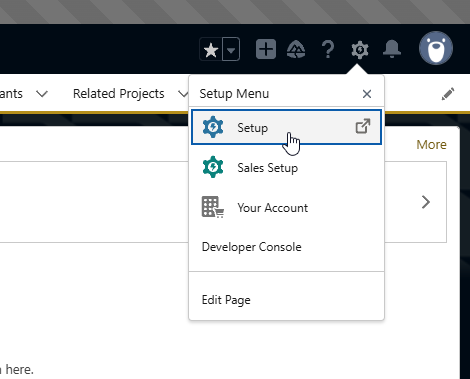
\includegraphics[width=0.8\textwidth]{Chapter4/Pictures/Setup.png} % Replace with actual figure file
            \caption{Salesforce Setup Menu}
            \label{fig:create_app1}
        \end{figure}

         \begin{figure}[h!]
            \centering
            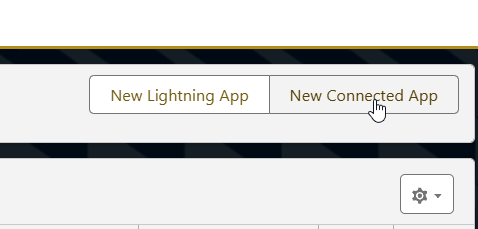
\includegraphics[width=0.8\textwidth]{Chapter4/Pictures/con_app.png} % Replace with actual figure file
            \caption{Creating a New Connected App in Salesforce}
            \label{fig:create_app2}
        \end{figure}
    \end{itemize}

    \item \textbf{Provide Basic Details:}
    \begin{itemize}
        \item On the next screen, fill in the required fields, including \textbf{App Name}, \textbf{API Name}, and \textbf{Contact Email}. Enable OAuth Settings by selecting the appropriate checkbox (see Figure 4.2).
        \begin{figure}[h!]
            \centering
            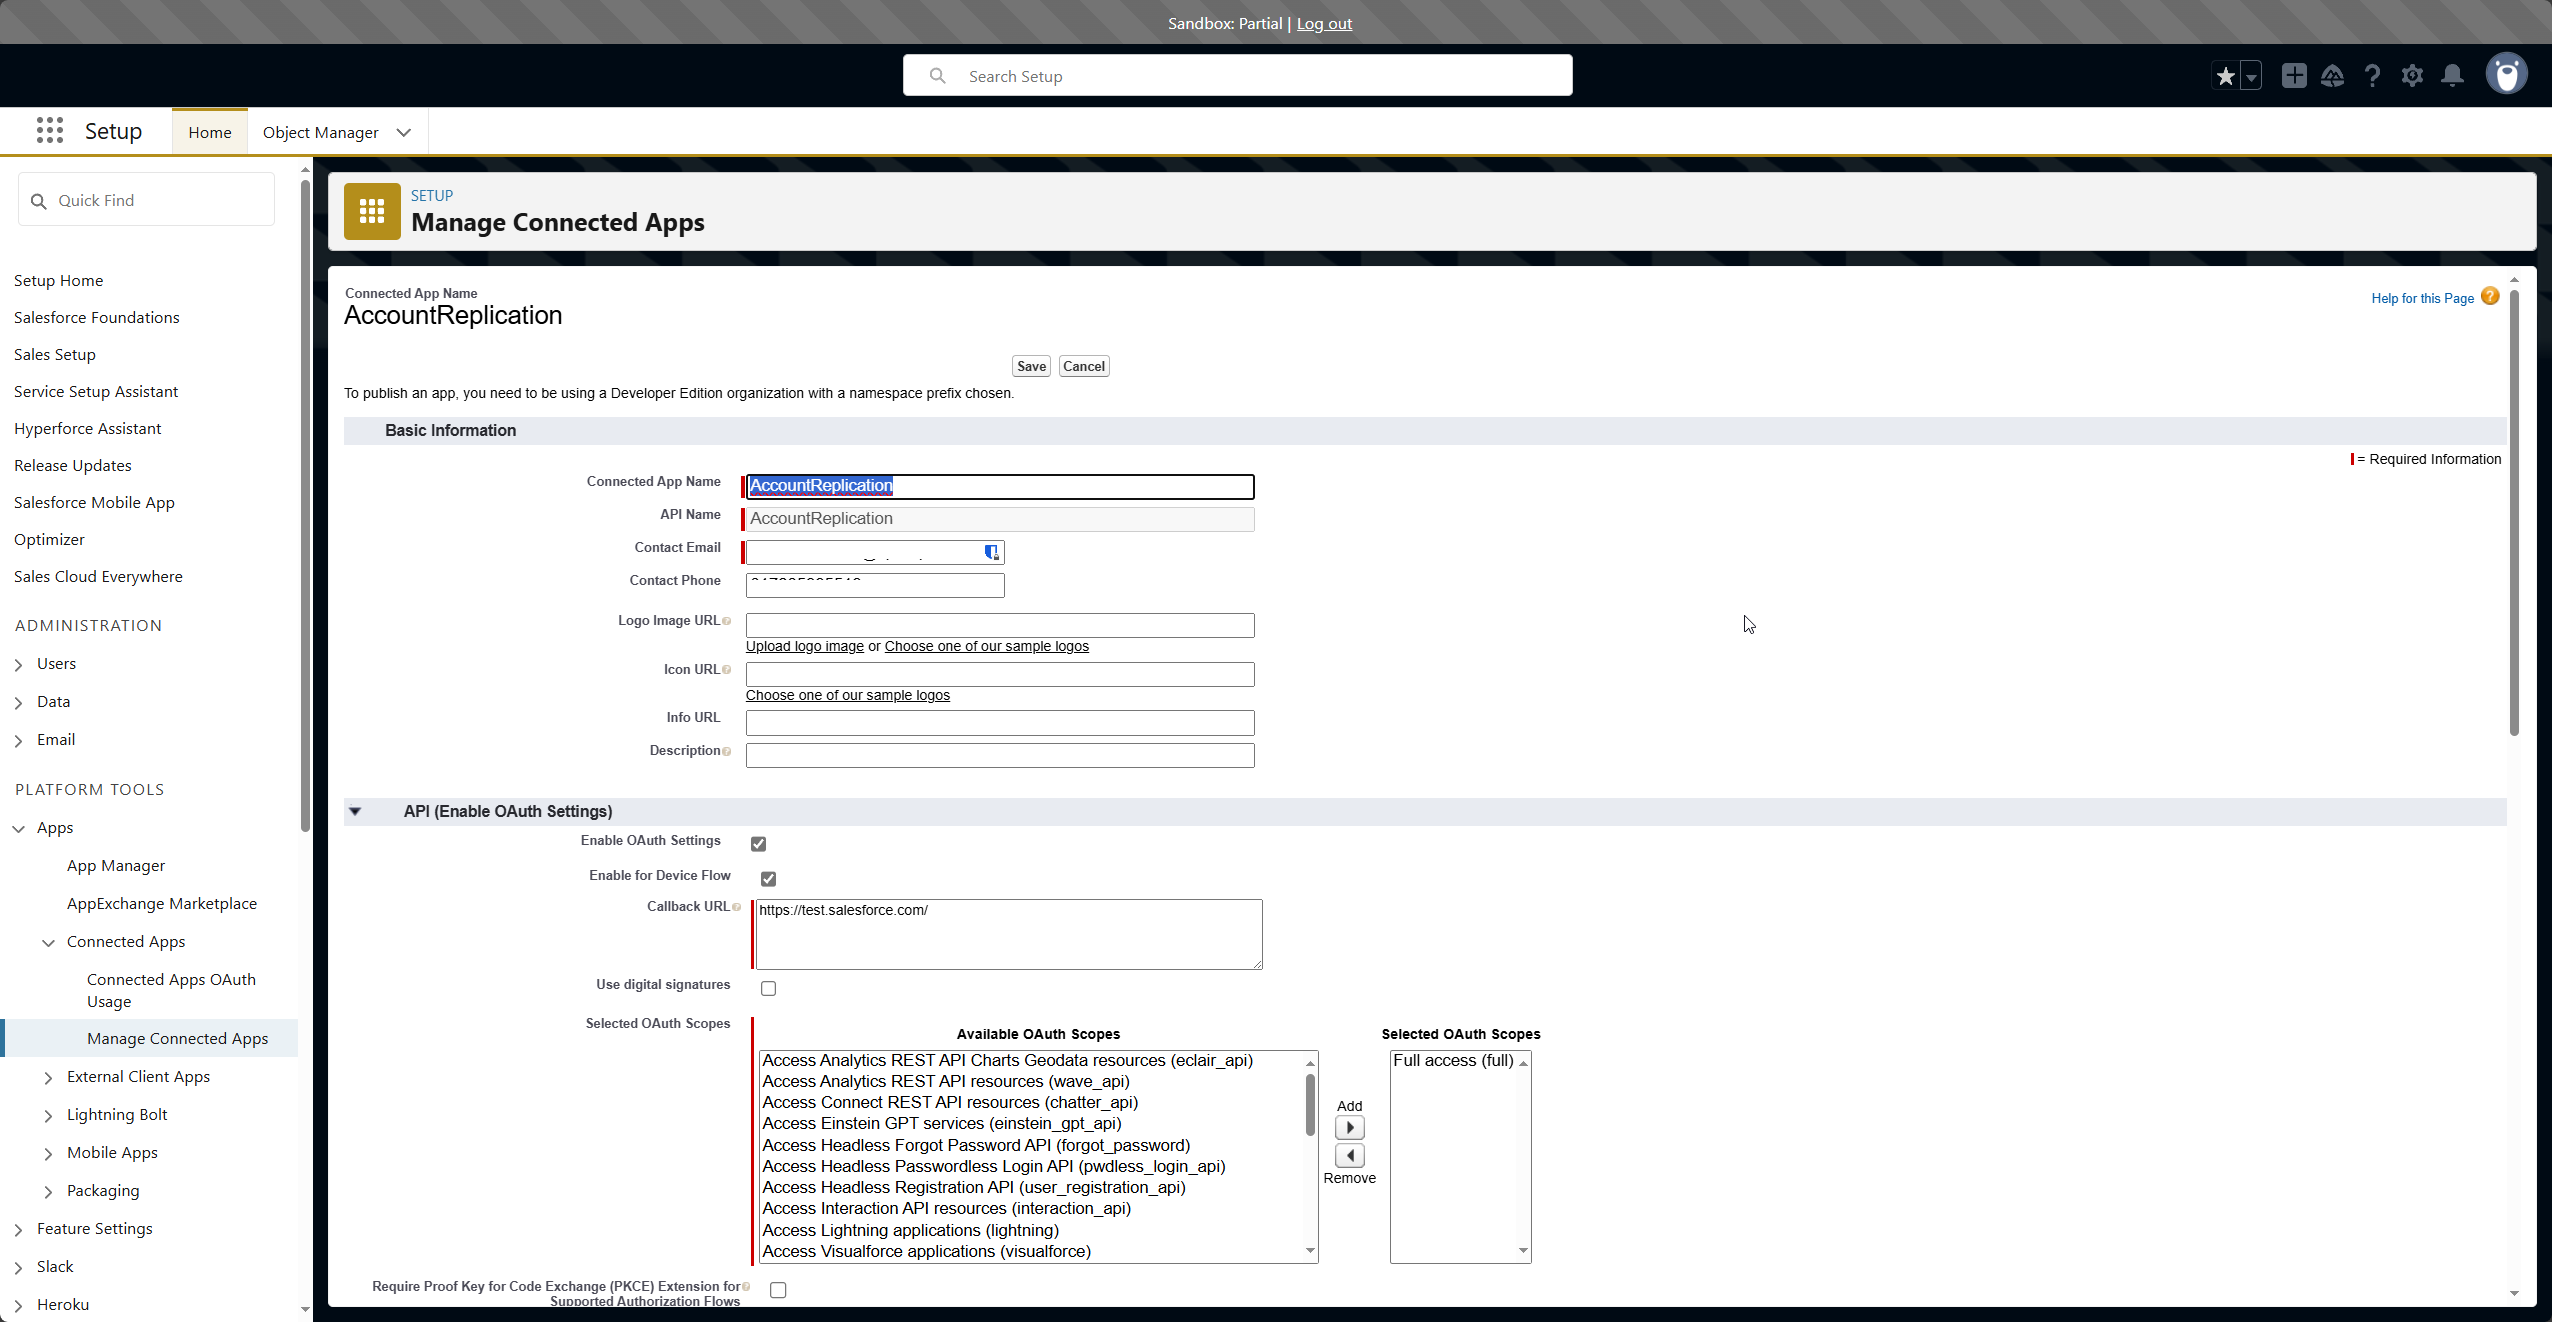
\includegraphics[width=0.8\textwidth]{Chapter4/Pictures/Connectedapp.png} % Replace with actual figure file
            \caption{Salesforce Connected App Configuration}
            \label{fig:new_app}
        \end{figure}
    \end{itemize}

    \item \textbf{Configure OAuth Settings:}
    \begin{itemize}
        \item In the API section (see Figure 4.3), perform the following actions:
        \begin{itemize}
            \item Disable \textbf{Enable for Device Flow}.
            \item Provide a \textbf{Callback URL}.
            \item Disable \textbf{Use digital signatures}.
            \item Set \textbf{Selected OAuth Scopes} to \textbf{Full access (full)}.
            \item Enable \textbf{Require Secret for Web Server Flow}.
            \item Disable \textbf{Include ID Token}.
            \item Disable \textbf{Enable Asset Tokens}.
        \end{itemize}
        \item Save the configuration to complete the creation of the Connected App.

    \end{itemize}

    \item \textbf{Retrieve Client ID and Client Secret:}
    \begin{itemize}
        \item Once the app is created, navigate to the app overview. The \textbf{Client ID} and \textbf{Client Secret} can be found in the \textbf{Consumer Key} and \textbf{Consumer Secret} fields, respectively (see Figure 4.4).

    \begin{figure}[H]
    \centering
    \fbox{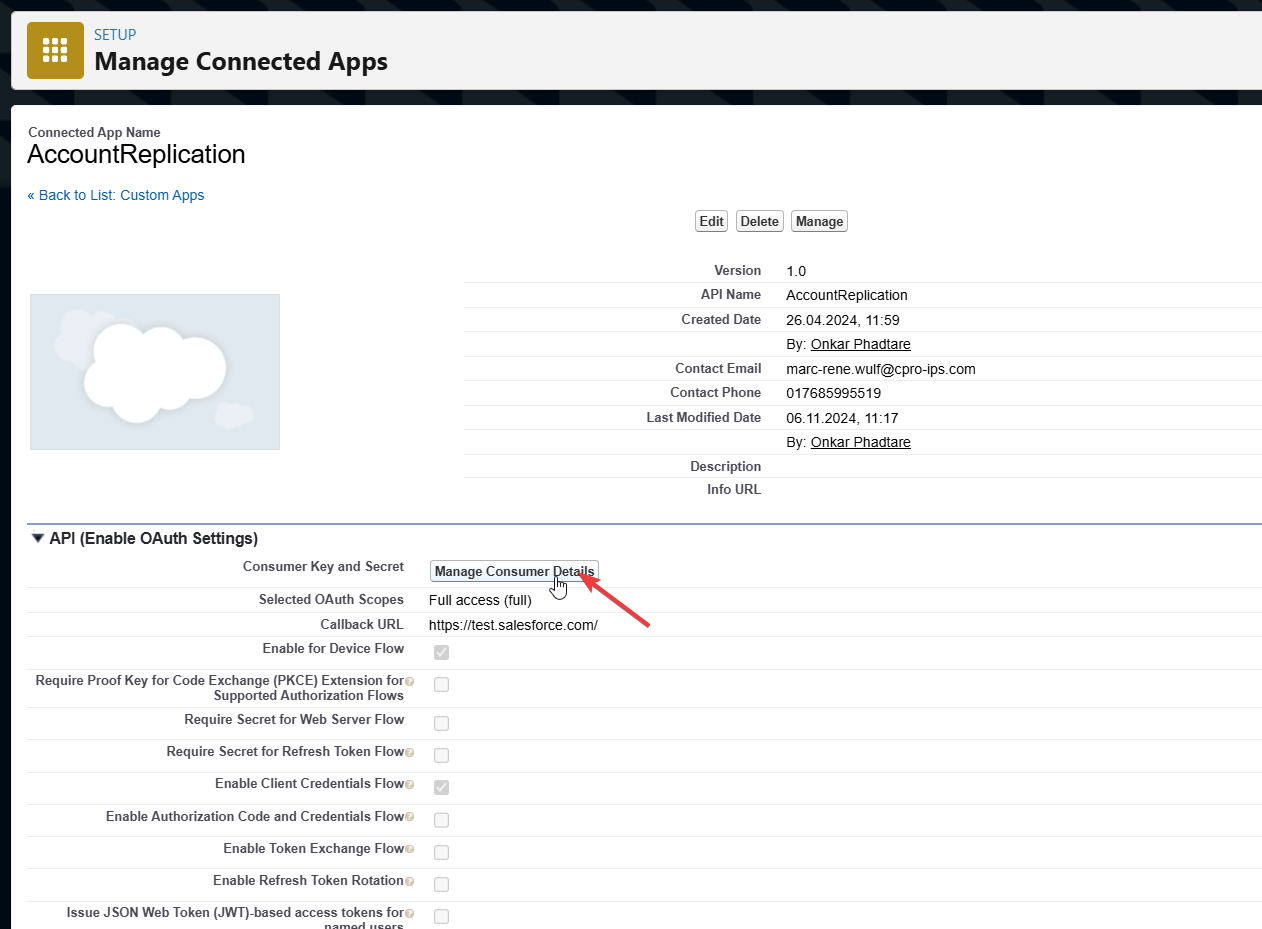
\includegraphics[width=0.8\textwidth]{Chapter4/Pictures/API.png}}
    \caption{OAuth Settings for Salesforce Connected App}
    
    \end{figure}

    \end{itemize}
\end{enumerate}


\subsubsection{Adding SAP S/4HANA References}
The integration content facilitates the synchronization of data between SAP S/4HANA Cloud and Salesforce. To achieve this, it is necessary to create unique identifiers in Salesforce that store key values from SAP S/4HANA Cloud. These identifiers, referred to as External IDs, enable accurate mapping and synchronization of records between the two systems. The following procedure outlines the steps required to add these references in Salesforce.

\paragraph{Procedure}
\begin{enumerate}
    \item \textbf{Access the Setup Screen:}
    \begin{itemize}
        \item Navigate to the Salesforce Setup menu to begin the configuration process.
    \end{itemize}

    \item \textbf{Locate the Object Fields:}
    \begin{itemize}
        \item In the Quick Find search box, type \texttt{Accounts*} and select \texttt{Fields} from the search results.
    \end{itemize}

    \begin{figure}[H]
    \centering
    \fbox{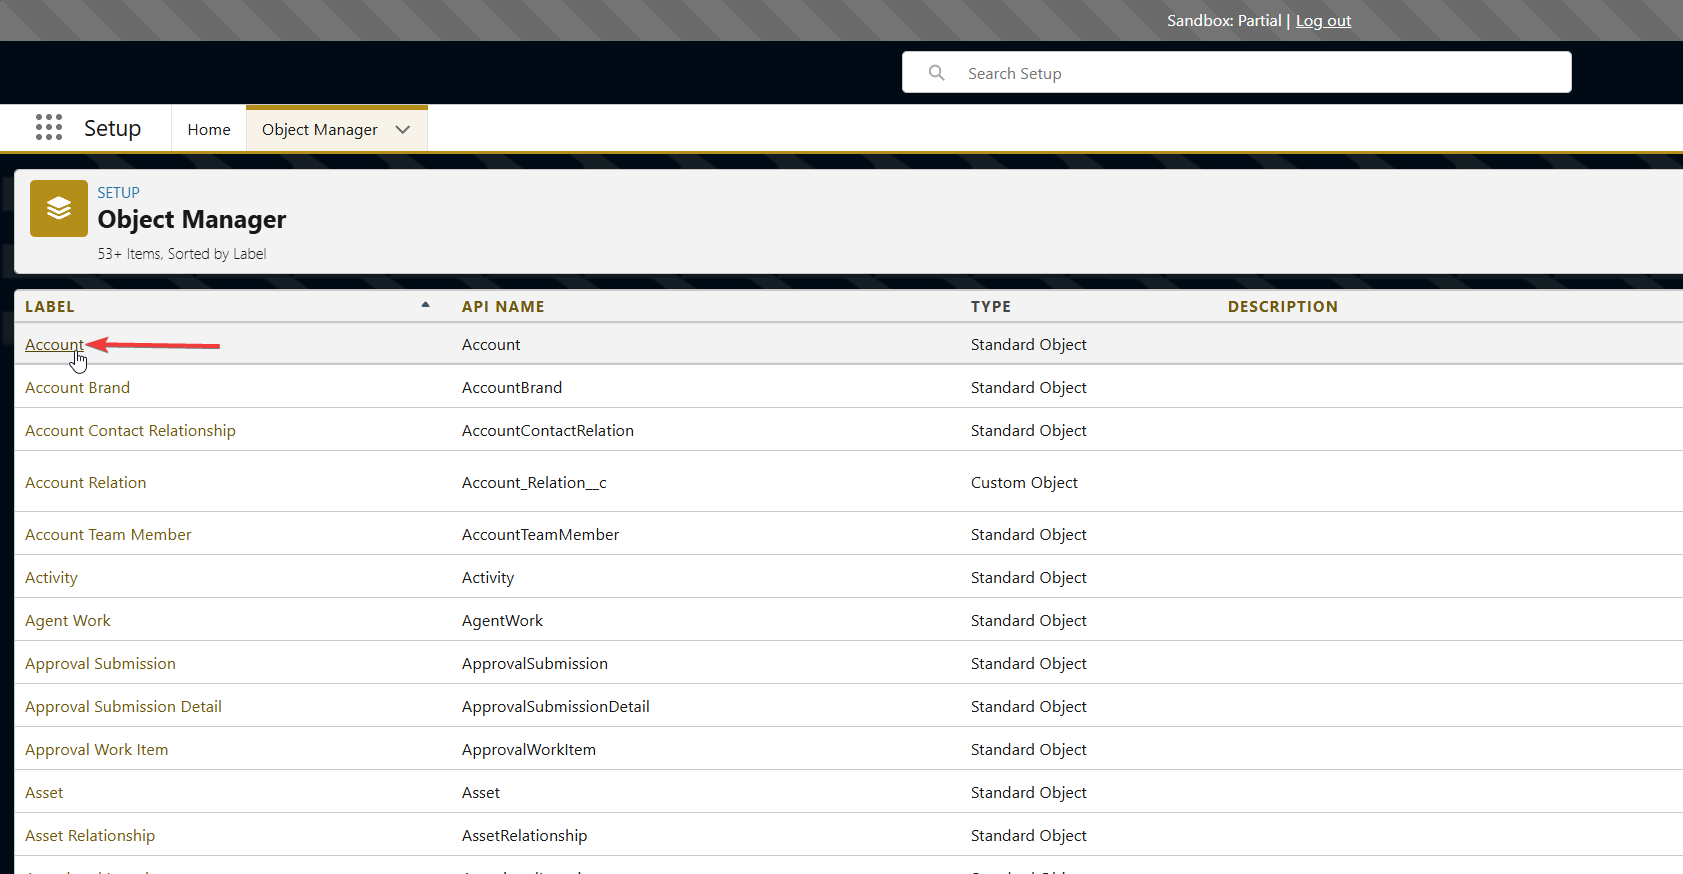
\includegraphics[width=0.8\textwidth]{Chapter4/Pictures/fieldsetup.png}}
    \caption{Salesforce Object Manager}
    
    \end{figure}

    \item \textbf{Create a New Field:}
    \begin{itemize}
        \item Scroll down and click the \texttt{New} button to initiate the creation of a new custom field.
    \end{itemize}

    \item \textbf{Select Field Type:}
    \begin{itemize}
        \item Choose \texttt{Text} as the field type and proceed by clicking \texttt{Next}.
    \end{itemize}

    \item \textbf{Define Field Properties:}
    \begin{itemize}
        \item Enter the field name as \texttt{SAP\_BusinessPartner\_Ref}, specify a length of \texttt{30 characters}, and enable the \texttt{External ID} checkbox. This ensures that the field can uniquely identify records from SAP S/4HANA Cloud.
    \end{itemize}
    
    \begin{figure}[H]
    \centering
    \fbox{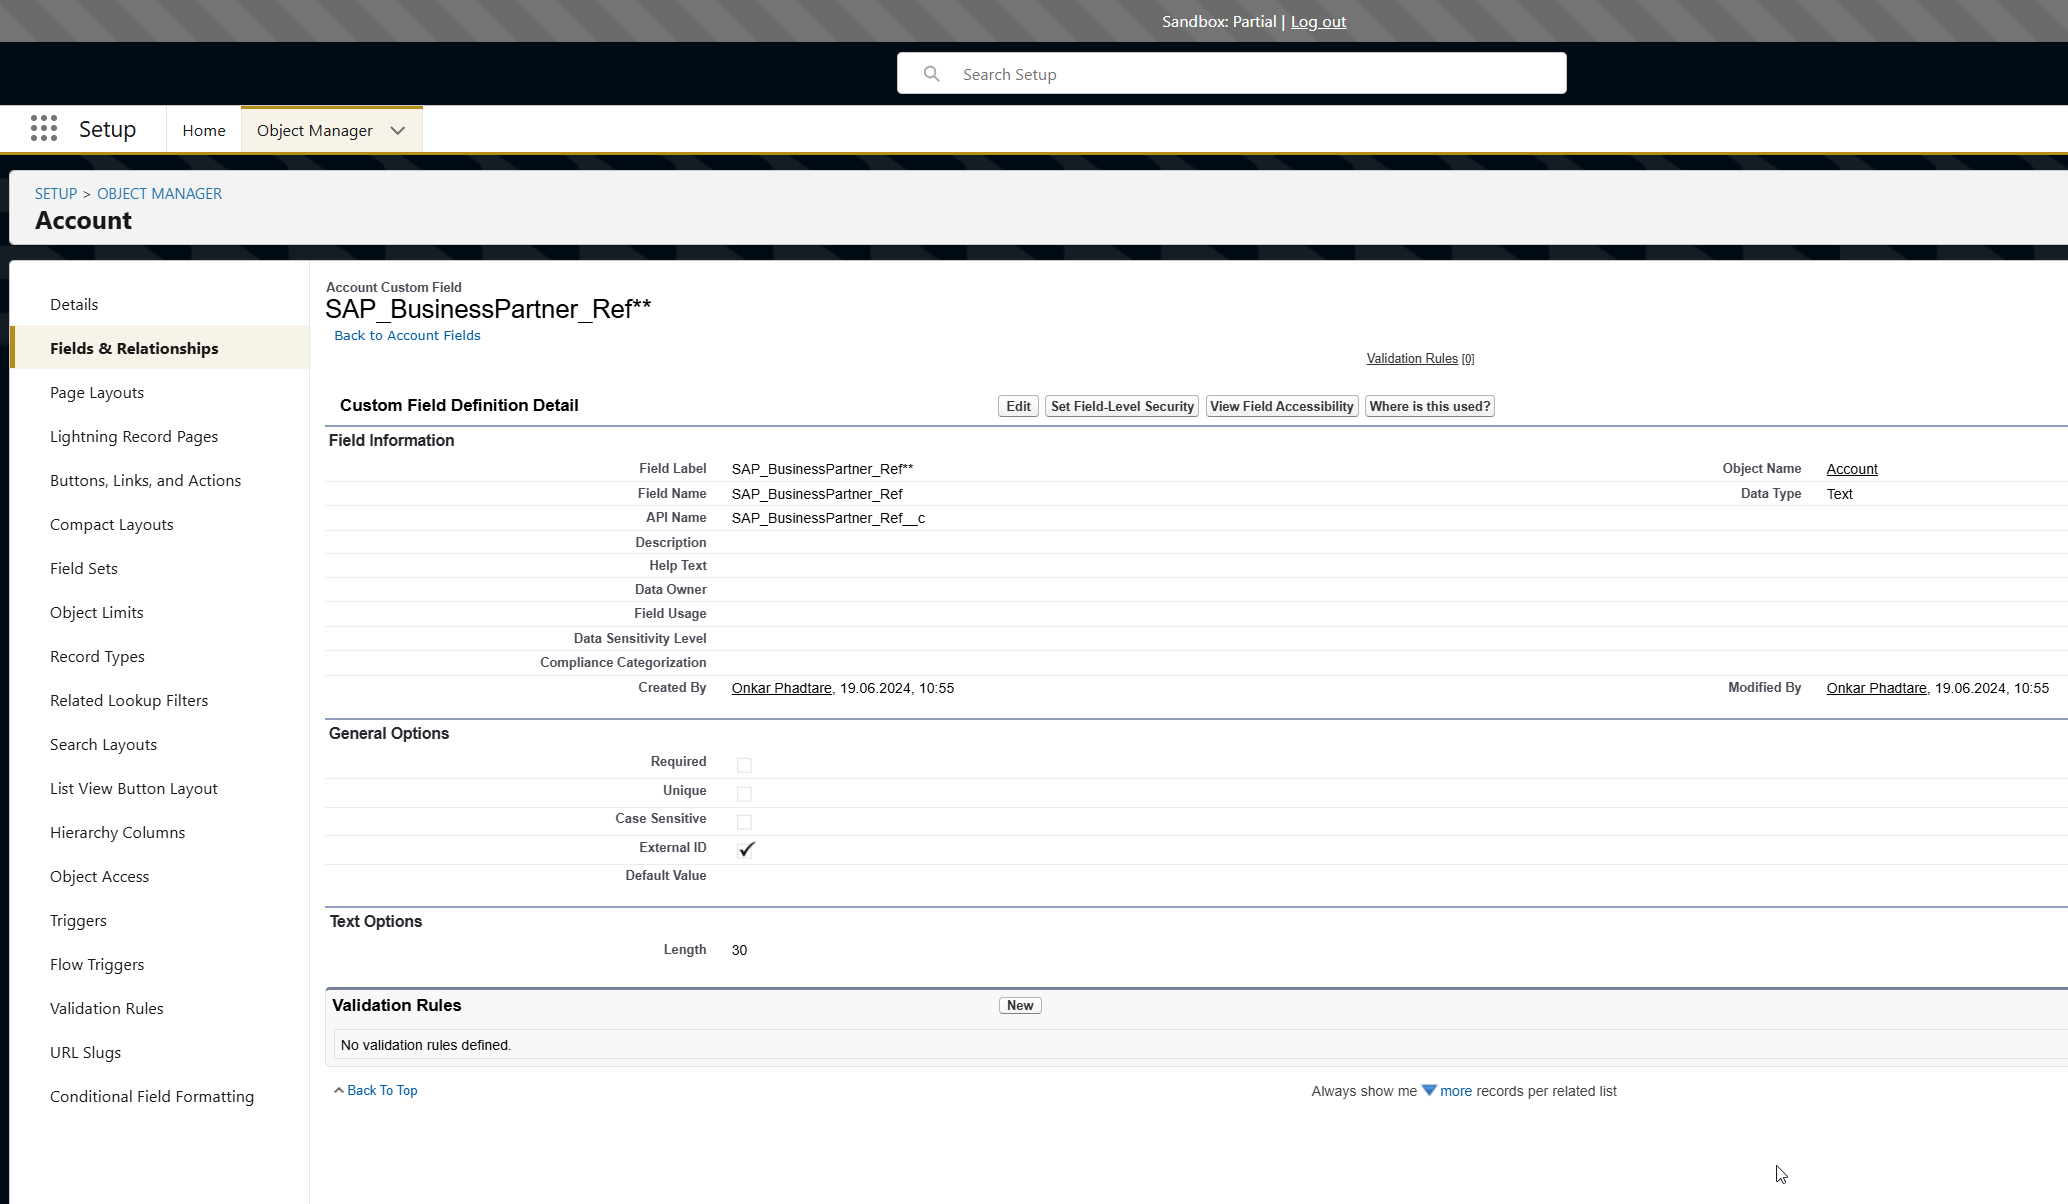
\includegraphics[width=0.8\textwidth]{Chapter4/Pictures/fieldlen.png}}
    \caption{Reference Field Details}
    
    \end{figure}
    

    \item \textbf{Complete Field Creation:}
    \begin{itemize}
        \item Click \texttt{Next} twice to proceed through the configuration screens, and then save the field.
    \end{itemize}

    \begin{figure}[H]
    \centering
    \fbox{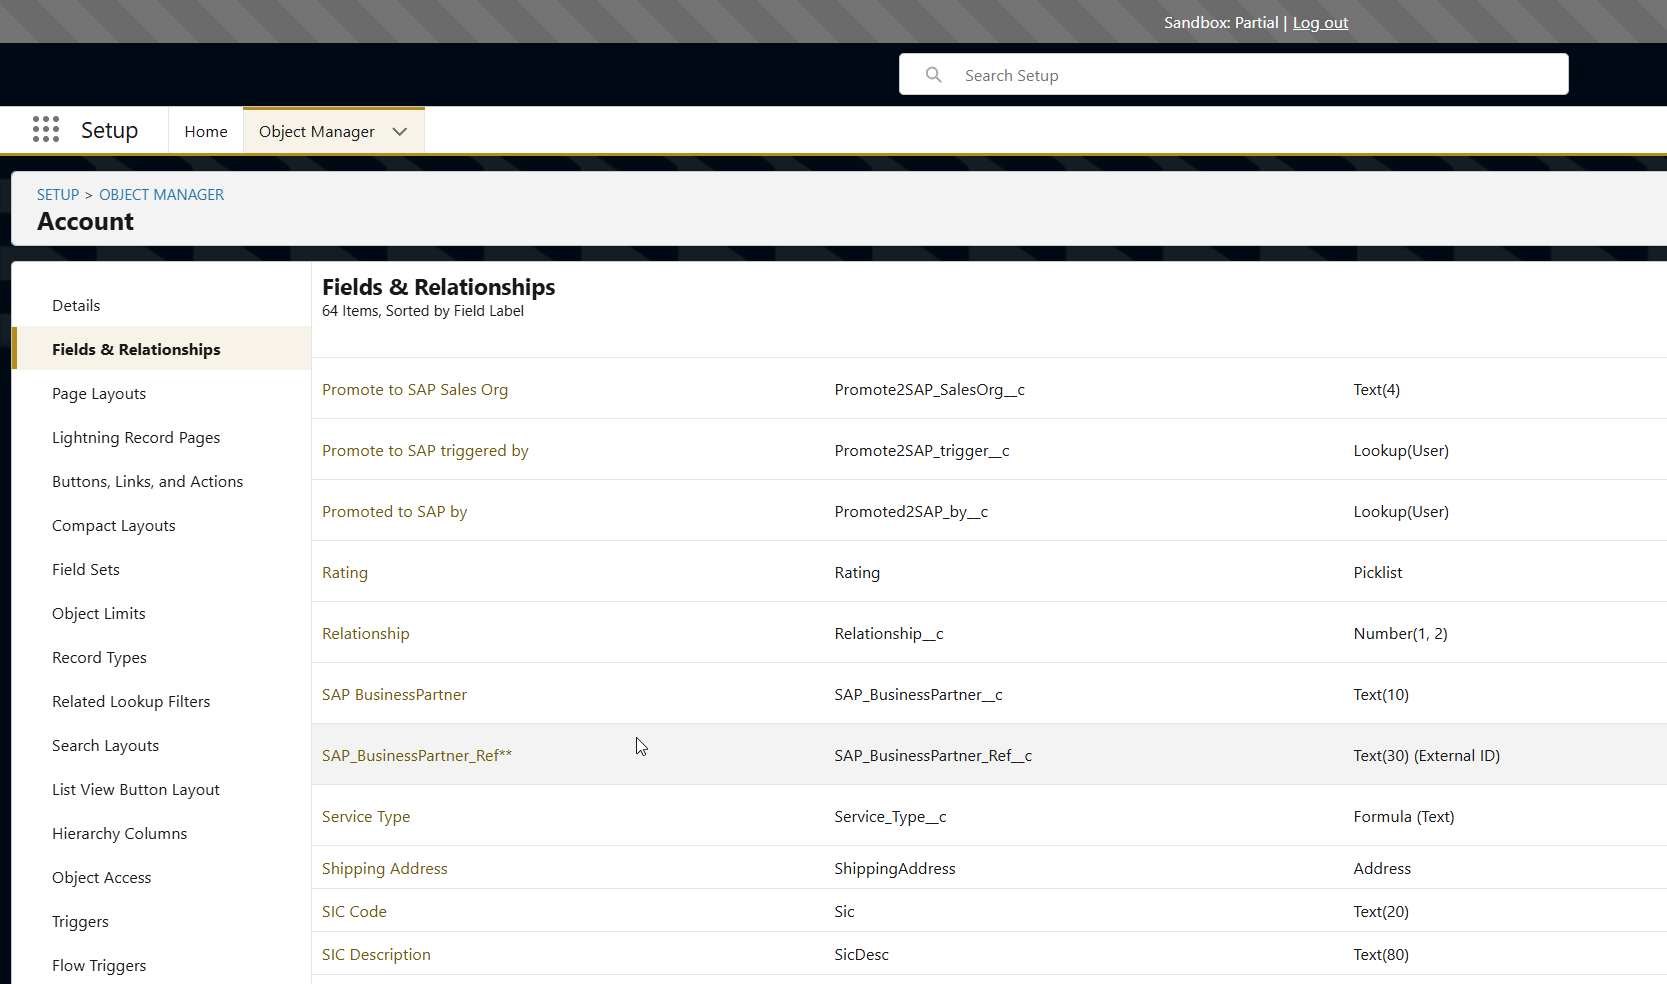
\includegraphics[width=0.8\textwidth]{Chapter4/Pictures/ref.png}}
    \caption{SAP BTP Integration Flow for Account Replication}
    
    \end{figure}

    \item \textbf{Repeat for Additional Objects:}
    \begin{itemize}
        \item The above steps must be repeated for other Salesforce objects to create corresponding External ID fields. Below is a table listing the required fields for each object:
    \end{itemize}
\end{enumerate}

\subparagraph{Required Fields for Objects}
\begin{table}[h!]
    \centering
    \begin{tabular}{|l|l|}
        \hline
        \textbf{Object}          & \textbf{Field Name}              \\ \hline
        Products                  & SAP\_Material\_Ref               \\ \hline
        Accounts                  & SAP\_BusinessPartner\_Ref        \\ \hline
        Orders                    & SAP\_SalesOrder\_Ref             \\ \hline
        Order Products            & SAP\_OrderItem\_Ref              \\ \hline
        Service Contracts         & SAP\_SalesContract\_Ref          \\ \hline
        Contract Line Items       & SAP\_SalesContractItem\_Ref      \\ \hline
        Price Book Entries        & SAP\_PriceBookEntry\_Ref         \\ \hline
    \end{tabular}
    \caption{Required External ID Fields for Salesforce Objects}
    \label{tab:external_ids}
\end{table}

By following this procedure, the necessary External ID fields are created in Salesforce, enabling the integration content to synchronize data accurately between SAP S/4HANA Cloud and Salesforce. This step is critical for ensuring data consistency and alignment across the integrated systems.


\subsection{Configuration in SAP Cloud Platform Integration }

This section discusses the configuration of Integration Flows (iFlows) within SAP Cloud Platform Integration (CPI), focusing on the prerequisites, sender and receiver system parameters, and iFlow-specific settings. Prerequisites include ensuring access permissions, credentials, and system configurations for both sender (e.g., SAP S/4HANA) and receiver (e.g., Salesforce) systems. Sender system parameters define data sources, communication protocols, and authentication mechanisms, while receiver system parameters configure endpoints, data transformation rules, and authentication details. Additionally, iFlow-specific settings, such as message mappings and exception handling, are tailored to each use case. Proper configuration of these elements ensures robust and efficient data exchange, enabling seamless integration and process automation between systems.


\subsubsection{Procedure for Deploying User Credentials}

\begin{enumerate}
    \item \textbf{Accessing the Monitoring Section:}
    \begin{itemize}
        \item Navigate to the \textbf{Monitor} tab within your SAP CPI tenant to access system monitoring and configuration settings.
    \end{itemize}
    
    \item \textbf{Managing Security Configurations:}
    \begin{itemize}
        \item Under the \textbf{Manage Security} section, select \textbf{Security Material} to access the repository where authentication-related configurations are stored.
    \end{itemize}
    
    \item \textbf{Adding New User Credentials:}
    \begin{itemize}
        \item Click on the \textbf{Add} dropdown menu and choose \textbf{User Credentials} as the authentication method.
    \end{itemize}
    
    \item \textbf{Entering Authentication Details:}
    \begin{itemize}
        \item Provide a unique \textbf{Name} for the credentials, ensuring they can be referenced in integration flows.
        \item Enter the \textbf{Salesforce username} and \textbf{password} associated with the account that will be used for authentication.
    \end{itemize}
    
    \item \textbf{Deploying the Credentials:}
    \begin{itemize}
        \item Click on \textbf{Deploy} to securely store and activate the credentials for use within the integration process.
    \end{itemize}
\end{enumerate}

\subsubsection{Procedure for Deploying Token}

To securely store and utilize authentication tokens within \textbf{SAP Cloud Platform Integration (SAP CPI)}, it is essential to deploy the token using the \textit{Secure Parameter} functionality. This ensures that sensitive credentials, such as a Salesforce token, are securely managed within the SAP CPI environment. The following steps outline the procedure to configure and deploy the secure parameter for authentication:

\begin{enumerate}
    \item \textbf{Access the SAP CPI Tenant}: \\
    Log in to the \textbf{SAP Cloud Platform Integration (CPI)} tenant and navigate to the \textit{Monitor} section to access system management tools.
    
    \item \textbf{Navigate to Security Management}: \\
    Within the \textit{Monitor} section, locate and click on \textit{Manage Security}. From the available options, select \textit{Security Material} to manage authentication credentials.
    
    \item \textbf{Add a Secure Parameter}: \\
    Click on the \textit{Add} dropdown menu and select \textit{Secure Parameter} from the list of available security material types.
    
    \item \textbf{Configure the Secure Parameter}: \\
    In the configuration screen, provide a meaningful \textit{Name} for the secure parameter. This name will be used in integration flows (iFlows) to reference the stored token. Enter the \textbf{Salesforce authentication token} in the \textit{Secure Parameter} field. This ensures that the token is securely stored and can be retrieved dynamically during API authentication.
    
    \item \textbf{Deploy the Secure Parameter}: \\
    Click on the \textit{Deploy} button to save and activate the secure parameter within the SAP CPI environment. Upon successful deployment, the secure parameter becomes available for use in \textit{integration flows (iFlows)}, enabling secure and seamless authentication when interacting with external systems, such as Salesforce.
\end{enumerate}

By following this structured approach, organizations can ensure the \textbf{secure storage and management of authentication tokens}, thereby enhancing the security and compliance of their integration processes within SAP CPI.



\subsubsection{Replicate Account from SAP S/4HANA to Salesforce}

This integration flow facilitates the replication of customer master data from SAP S/4HANA to Salesforce, where the data is mapped to the Accounts object. Whenever a customer record is created or modified in SAP S/4HANA, the changes are automatically replicated to Salesforce during the next execution of the integration flow, provided it is scheduled to run recurrently. This process ensures that Salesforce remains synchronized with the latest customer data from SAP S/4HANA. Figure 4.5 illustrates the business process implemented through this integration flow, highlighting the seamless data transfer and synchronization between the two systems.

    \begin{figure}[H]
    \centering
    \fbox{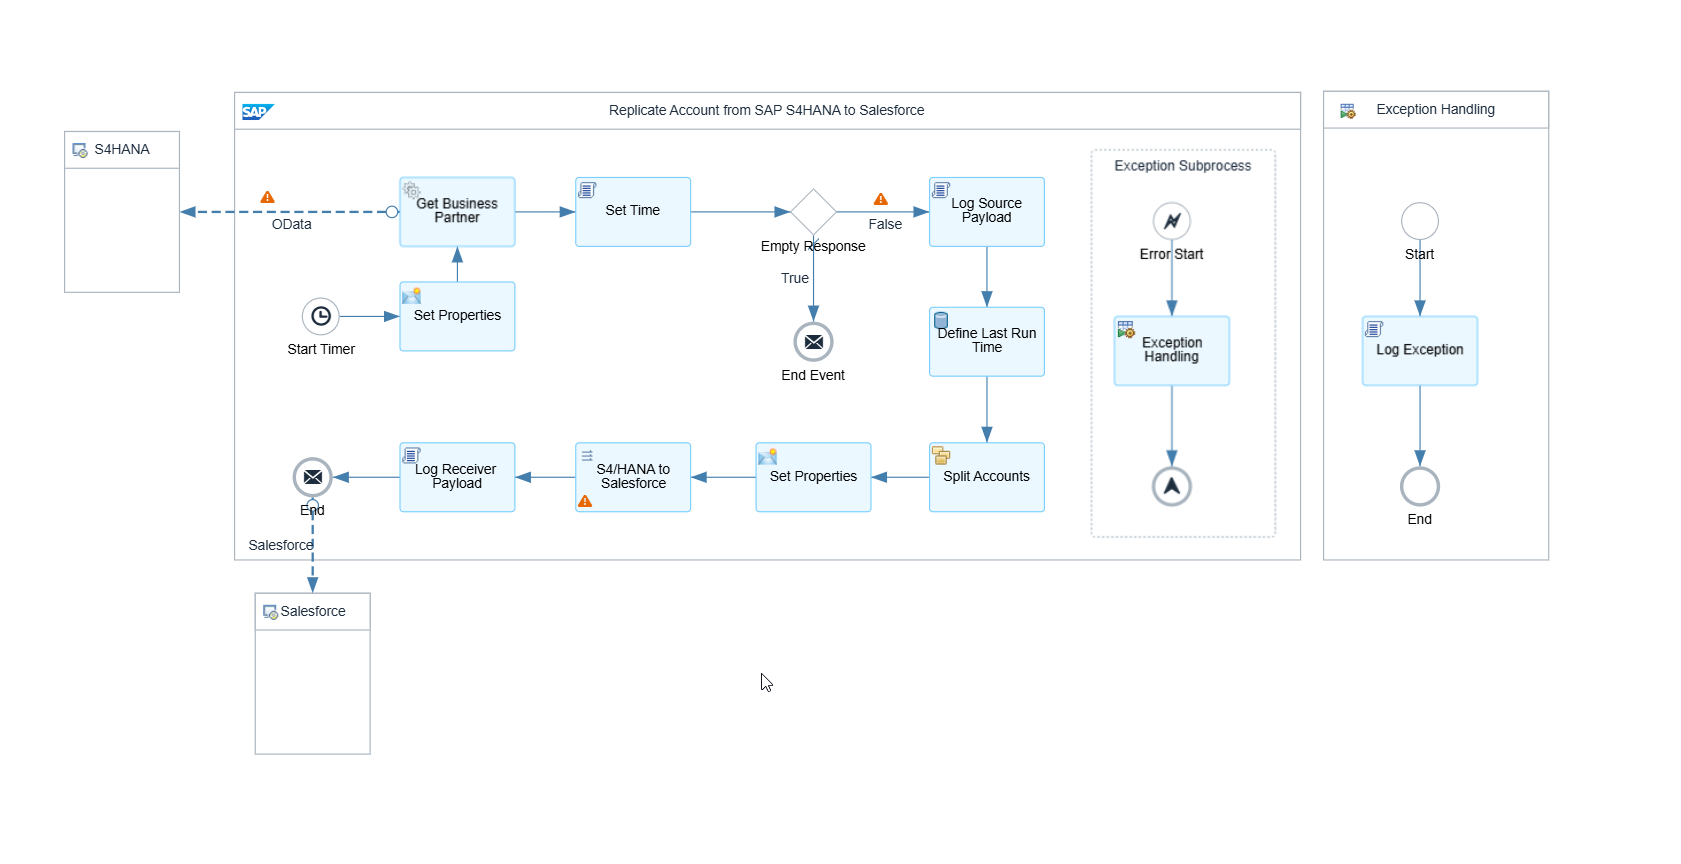
\includegraphics[width=0.8\textwidth]{Chapter4/Pictures/iflow.png}}
    \caption{Reference Field}
    
    \end{figure}


\paragraph{Prerequisites}
Before configuring the integration content, the following prerequisites must be addressed to ensure a smooth and successful implementation:

\begin{enumerate}
    \item \textbf{Deployment of Security Artifacts:}
    \begin{itemize}
        \item All necessary security artifacts, such as certificates, keys, and authentication tokens, must be deployed and configured. These artifacts are essential for establishing secure communication between SAP S/4HANA and Salesforce during the integration process.
    \end{itemize}

    
    \begin{figure}[H]
    \centering
    \fbox{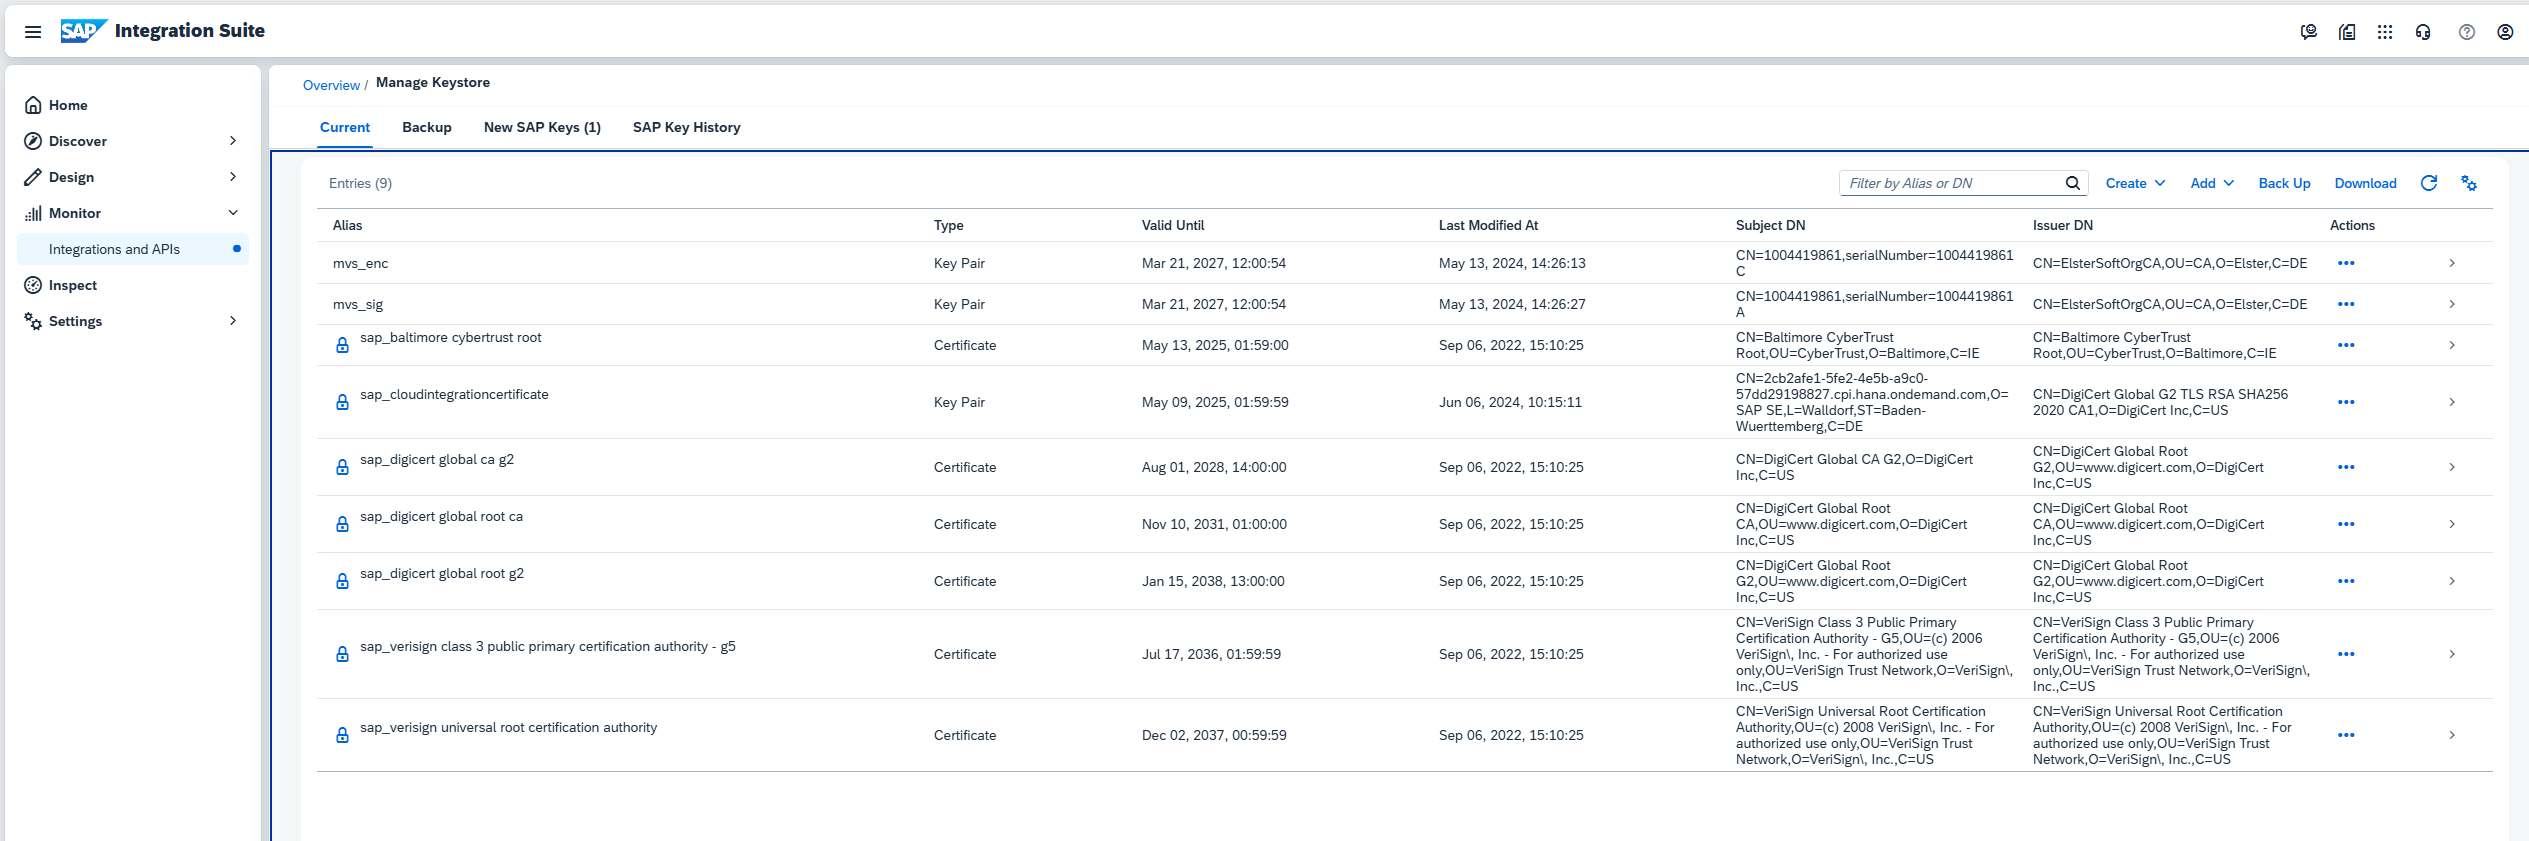
\includegraphics[width=0.8\textwidth]{Chapter4/Pictures/keys_certi.png}}
    \caption{Keys and Certificates in SAP Integration Suite}
    
    \end{figure}

    
    \begin{figure}[H]
    \centering
    \fbox{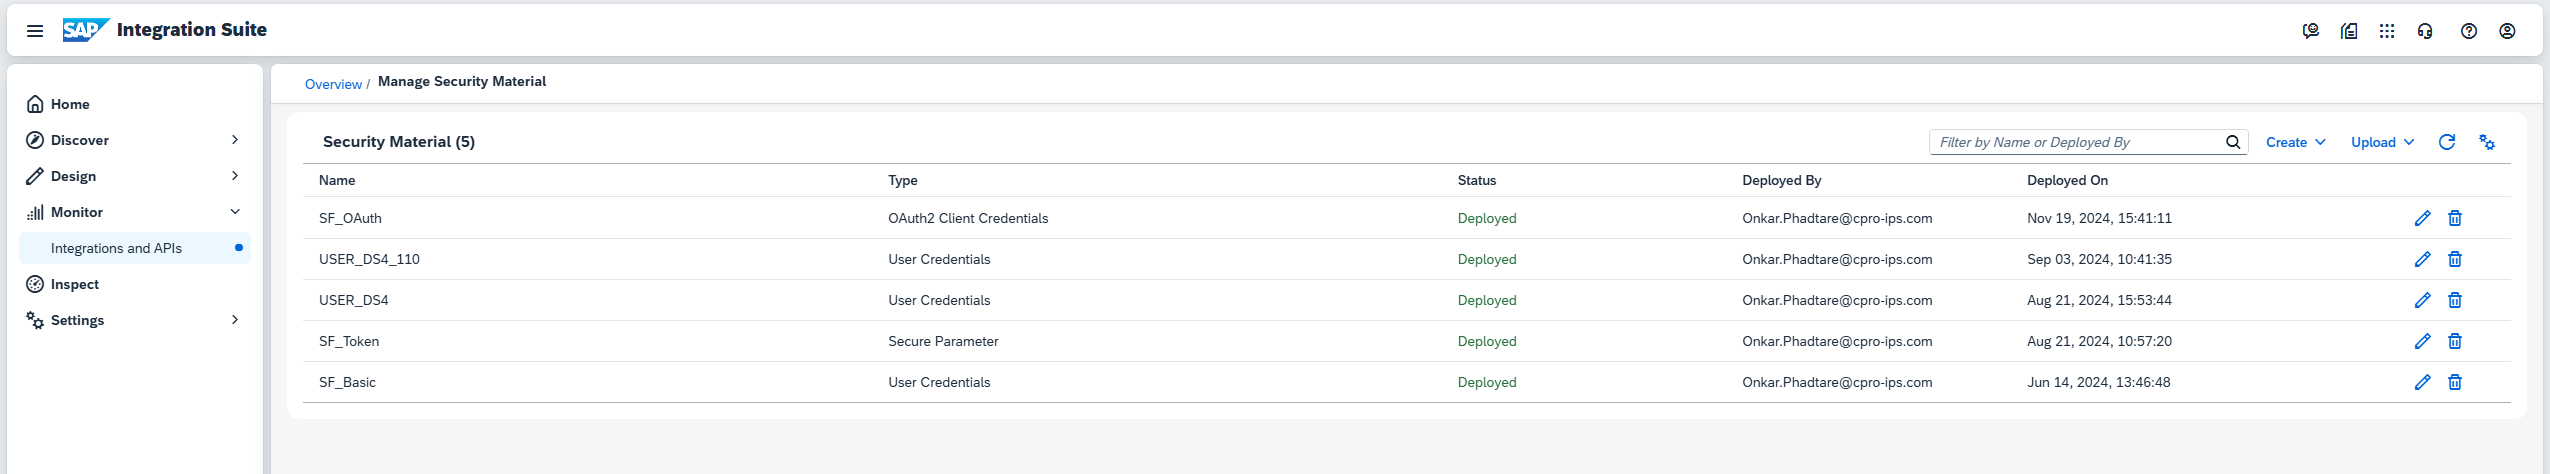
\includegraphics[width=0.8\textwidth]{Chapter4/Pictures/UserCred.png}}
    \caption{User Credentials in SAP Integration Suite}
    
    \end{figure}

    \item \textbf{Configuration of Time Zone and Initial Run Schedule:}
    \begin{itemize}
        \item Users must define the time zone in the configuration settings to ensure accurate scheduling and data replication. Additionally, the first run date and hour must be specified to determine when the integration flow should begin replicating data. This ensures that the replication process starts at the desired time and operates in the correct time context.
    \end{itemize}
\end{enumerate}

By fulfilling these prerequisites, the integration flow can be configured effectively, ensuring secure and timely replication of customer data from SAP S/4HANA to Salesforce.


\paragraph{Scope}
It is important to note that this integration flow is specifically designed to replicate Business Partners categorized as Customers from SAP S/4HANA to Salesforce. Business Partners belonging to other categories, such as vendors or suppliers, will not be included in the replication process. This ensures that only relevant customer data is synchronized between the two systems, maintaining data accuracy and alignment with the intended use case. The integration flow focuses exclusively on customer-related Business Partners, enabling efficient and targeted data replication for customer management in Salesforce.

\paragraph{Procedure } 

This section provides a step-by-step guide to configure the integration flow titled \textbf{"Replicate Account from SAP S/4HANA to Salesforce"}. The configuration process involves setting up the timer, configuring the receiver connectors for both SAP S/4HANA and Salesforce, and defining additional parameters under the "More" options. Below is a detailed explanation of each step:

\begin{enumerate}
    \item \textbf{Open the Integration Flow:}
    \begin{itemize}
        \item Begin by opening the integration flow \textbf{"Replicate Account from SAP S/4HANA to Salesforce"} in the SAP Cloud Platform Integration (CPI) interface. Click on the \textbf{Configure} button to proceed with the setup.
    \end{itemize}

    \begin{figure}[H]
    \centering
    \fbox{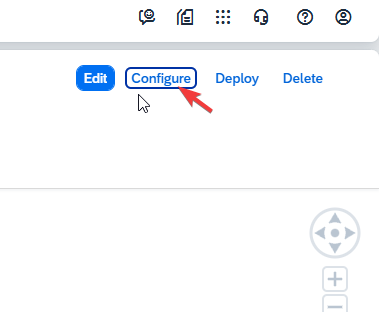
\includegraphics[width=0.8\textwidth]{Chapter4/Pictures/Configureiflow.png}}
    \caption{Configure the iFlow with Configure button}
    
    \end{figure}

    \item \textbf{Configure the Timer:}
    \begin{itemize}
        \item The timer determines the execution schedule of the integration flow. You can choose from the following options:
        \begin{itemize}
            \item \textbf{Run Once:} Executes the integration flow only once, typically used for initial data loads.
            \item \textbf{Schedule on Day:} Executes the integration flow on a specific date and time.
            \item \textbf{Schedule to Recur:} Executes the integration flow at regular intervals, ensuring continuous replication of changes from SAP S/4HANA to Salesforce. This is the recommended mode for ongoing synchronization.
        \end{itemize}
        \item Replace the default timer parameters with values appropriate for your specific scenario and system landscape.
    \end{itemize}

    \begin{figure}[H]
    \centering
    \fbox{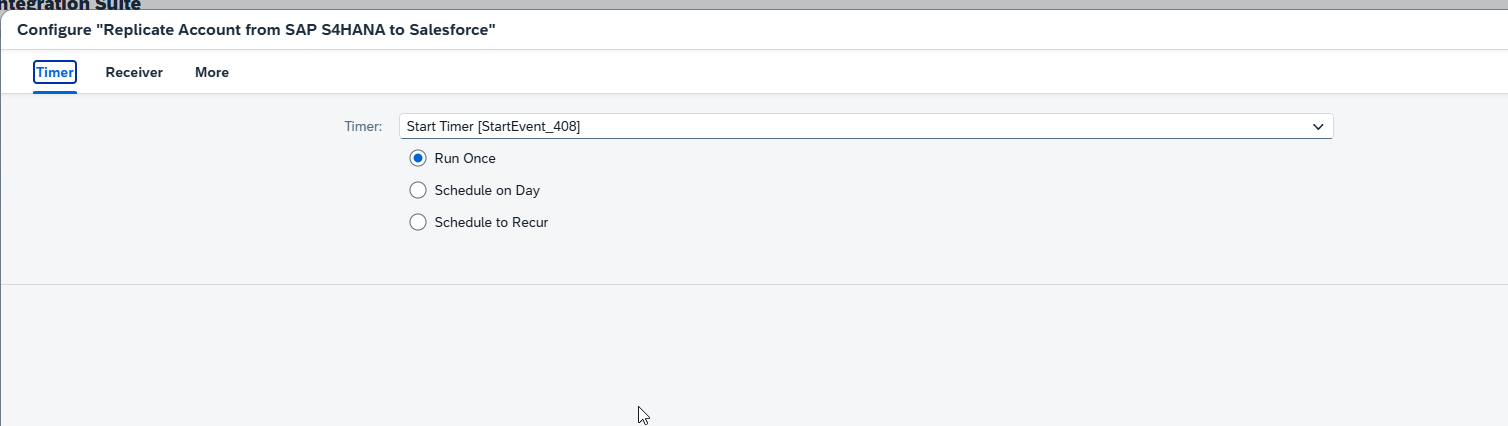
\includegraphics[width=0.8\textwidth]{Chapter4/Pictures/Schedule.png}}
    \caption{Timer Configuration in SAP Integration Suite}
    
    \end{figure}

    \item \textbf{Configure the SAP S/4HANA Receiver Connector:}
    \begin{itemize}
        \item Navigate to the \textbf{Receiver} section and configure the connector named \textbf{"S4HANA"}. The following parameters must be defined:
        \begin{itemize}
            \item \textbf{Hostname:} Enter the API hostname of your SAP S/4HANA system (e.g., \texttt{https://hostname:port/sap/opu/odata/sap/API\_BUSINESS\_PARTNER}).
            \item \textbf{Port:} Specify the API port of your SAP S/4HANA system.
            \item \textbf{Location ID:} Provide the location identifier for your SAP S/4HANA tenant.
            \item \textbf{Credential Name:} Enter the name of the credential artifact deployed for SAP S/4HANA authentication.
        \end{itemize}
    \end{itemize}


    \begin{figure}[H]
    \centering
    \fbox{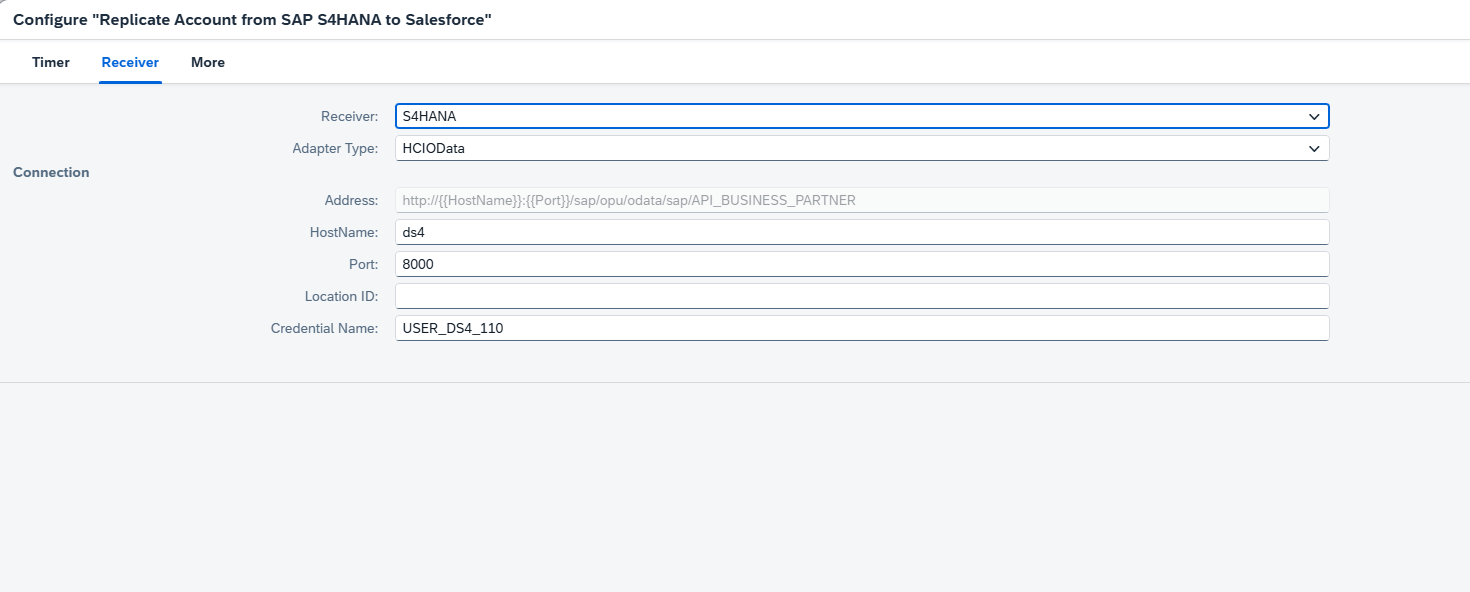
\includegraphics[width=0.8\textwidth]{Chapter4/Pictures/RecieverS4.png}}
    \caption{Receiver Configuration for SAP S/4HANA in SAP Integration Suite:}
    
    \end{figure}

    \item \textbf{Configure the Salesforce Receiver Connector:}
    \begin{itemize}
        \item Configure the connector named \textbf{"Salesforce"} with the following parameters:
        \begin{itemize}
            \item \textbf{Address:} Enter the data store URL for Salesforce (e.g., \texttt{https://login.salesforce.com}).
            \item \textbf{Basic Credential Name:} Specify the name of the deployed user credentials artifact containing the username and password for Salesforce authentication.
            \item \textbf{Security Token Alias:} Provide the name of the deployed secure parameter artifact holding the Salesforce security token, required for untrusted network access.
            \item \textbf{OAuth Credential Name:} Enter the name of the deployed OAuth credential artifact, if applicable.
        \end{itemize}
    \end{itemize}

    \begin{figure}[H]
    \centering
    \fbox{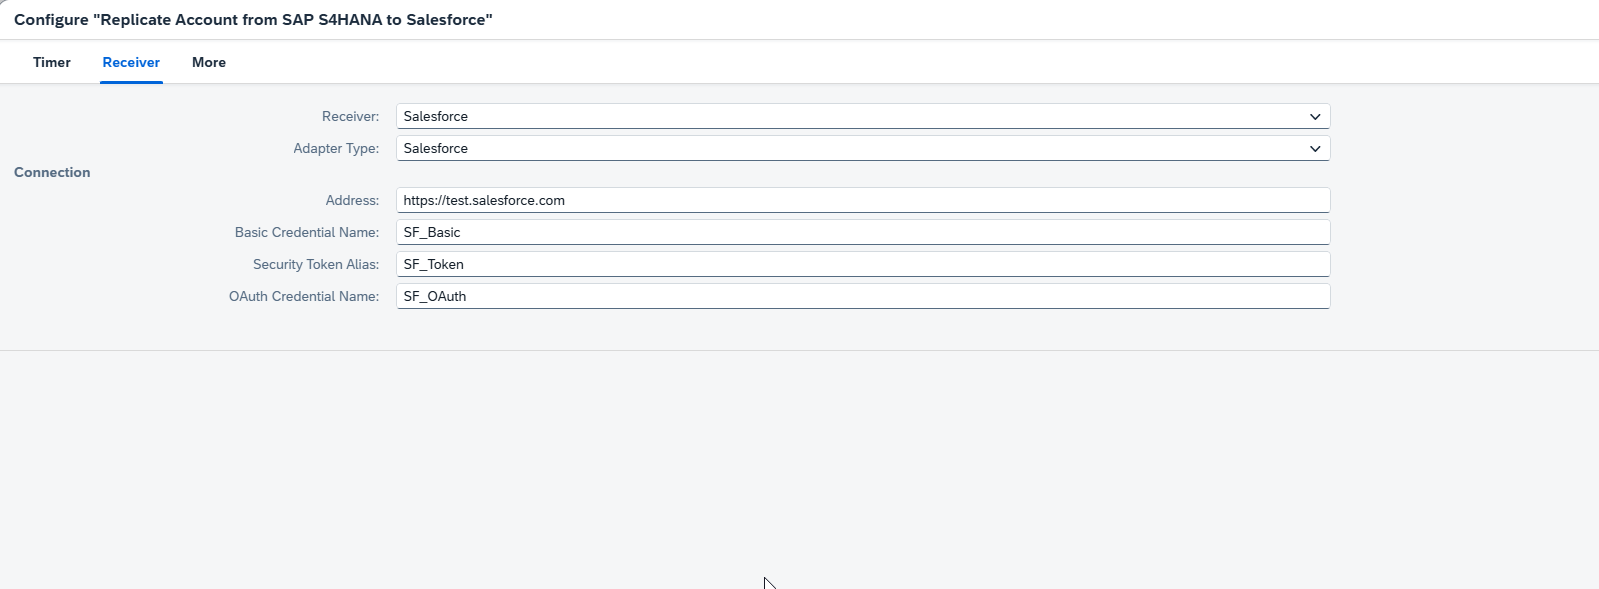
\includegraphics[width=0.8\textwidth]{Chapter4/Pictures/RecieverSF.png}}
    \caption{Receiver Configuration for Salesforce in SAP Integration Suite}
    
    \end{figure}

    \item \textbf{Configure Additional Options Under "More":}
    \begin{itemize}
        \item Under the \textbf{"More"} section, configure the following parameters:
        \begin{itemize}
            \item \textbf{ExceptionLogging:} Set to \textbf{"YES"} to log exceptions or \textbf{"NO"} to disable logging.
            \item \textbf{InitialDate:} Specify the start date for replication in the format \texttt{YYYY-MM-DD’T’hh:mm:ss.sss’Z’} (e.g., \texttt{1970-01-01T00:00:00.000Z}).
            \item \textbf{InitialHour:} Define the start time for replication in the format \texttt{‘PT’hh’H’mm’M’ss’S’} (e.g., \texttt{PT00H00M00S}).
            \item \textbf{LogMessageBody:} Set to \textbf{"YES"} to log the message body (not recommended for live environments) or \textbf{"NO"} to disable.
            \item \textbf{LogMessageHeader:} Set to \textbf{"YES"} to log the message header or \textbf{"NO"} to disable.
            \item \textbf{LogMessageProperty:} Set to \textbf{"YES"} to log message properties or \textbf{"NO"} to disable.
        \end{itemize}
    \end{itemize}

    \begin{figure}[H]
    \centering
    \fbox{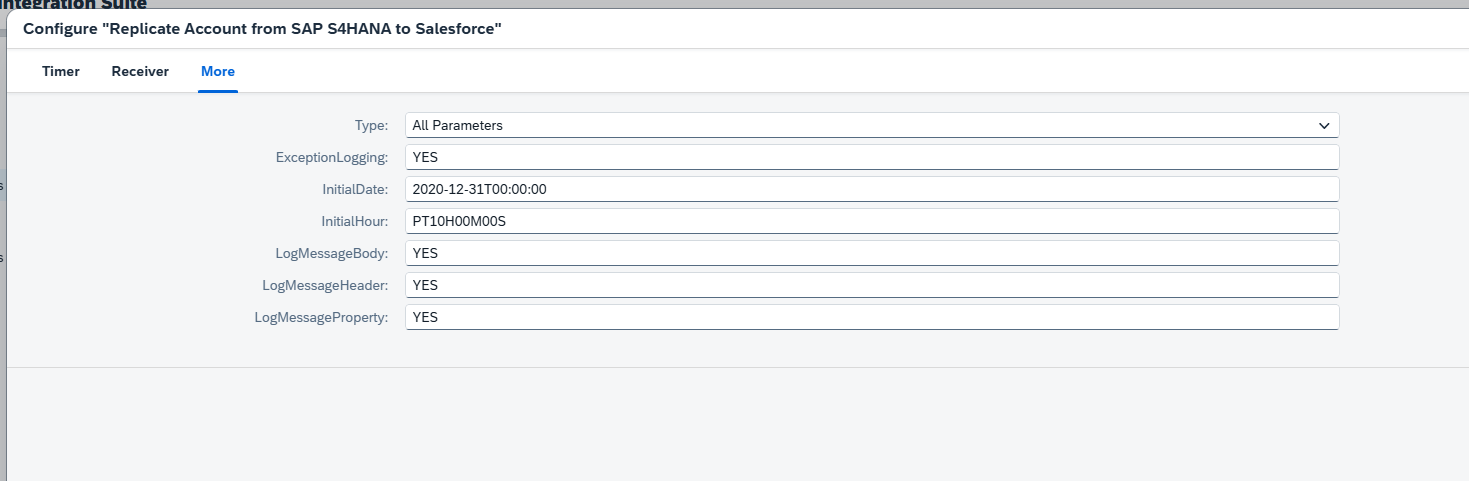
\includegraphics[width=0.8\textwidth]{Chapter4/Pictures/More.png}}
    \caption{Additional Configuration Settings in SAP Integration Suite}
    
    \end{figure}

    \item \textbf{Save and Deploy:}
    \begin{itemize}
        \item After completing the configuration, save the settings and deploy the integration flow. This activates the flow, enabling it to replicate customer data from SAP S/4HANA to Salesforce based on the defined schedule and parameters.
    \end{itemize}
\end{enumerate}


    \begin{figure}[H]
    \centering
    \fbox{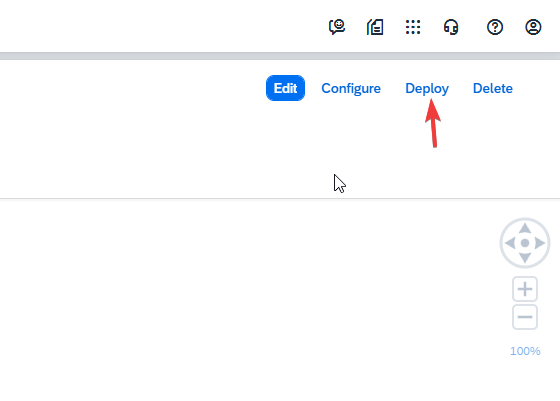
\includegraphics[width=0.8\textwidth]{Chapter4/Pictures/savedeploy.png}}
    \caption{Deploying the Integration Artifact in SAP Integration Suite}
    
    \end{figure}


This configuration process ensures that the integration flow operates efficiently, maintaining data consistency and alignment between SAP S/4HANA and Salesforce.




%=== END OF CHAPTER FOUR ===
\newpage
%=== CHAPTER FIVE (5) ===
%=== Discussion ===

\chapter{Integration Scenarios}
\section{Overview of Real-Time Integration}
This section provides a detailed overview of the real-time integration process between SAP S/4HANA, SAP CPI, and Salesforce, focusing on how data synchronization is achieved across these systems. The iFlow is specifically designed to facilitate the automated transfer of business-critical data, such as Business Partners (BP), from SAP S/4HANA to Salesforce, ensuring consistency and accuracy across platforms.

The integration process is structured into three key phases, each thoroughly examined to illustrate its role in the data exchange. These phases include data extraction and transmission from SAP S/4HANA, transformation and processing within SAP CPI, and API-based ingestion into Salesforce.

To enhance understanding, visual aids such as sequence diagrams, process flow charts, and screenshots are included. These illustrations help bridge technical explanations with real-world implementation, providing a clear representation of how data moves through the integration framework.

\subsection{Step 1: Business Partner Creation in SAP S/4HANA}

The integration process begins with the creation of a Business Partner (BP) in SAP S/4HANA, which serves as the foundation for maintaining customer and vendor records. SAP employs the BP concept to consolidate and streamline master data management, enabling seamless synchronization between SAP S/4HANA and external systems such as Salesforce.

\subsubsection{Accessing the Business Partner Transaction}
To create a new BP, users must navigate to the Business Partner (BP) transaction code in SAP S/4HANA:

\begin{enumerate}
    \item Open the SAP GUI and enter the transaction code \textbf{BP} in the command field.

    \begin{figure}[H]
    \centering
    \fbox{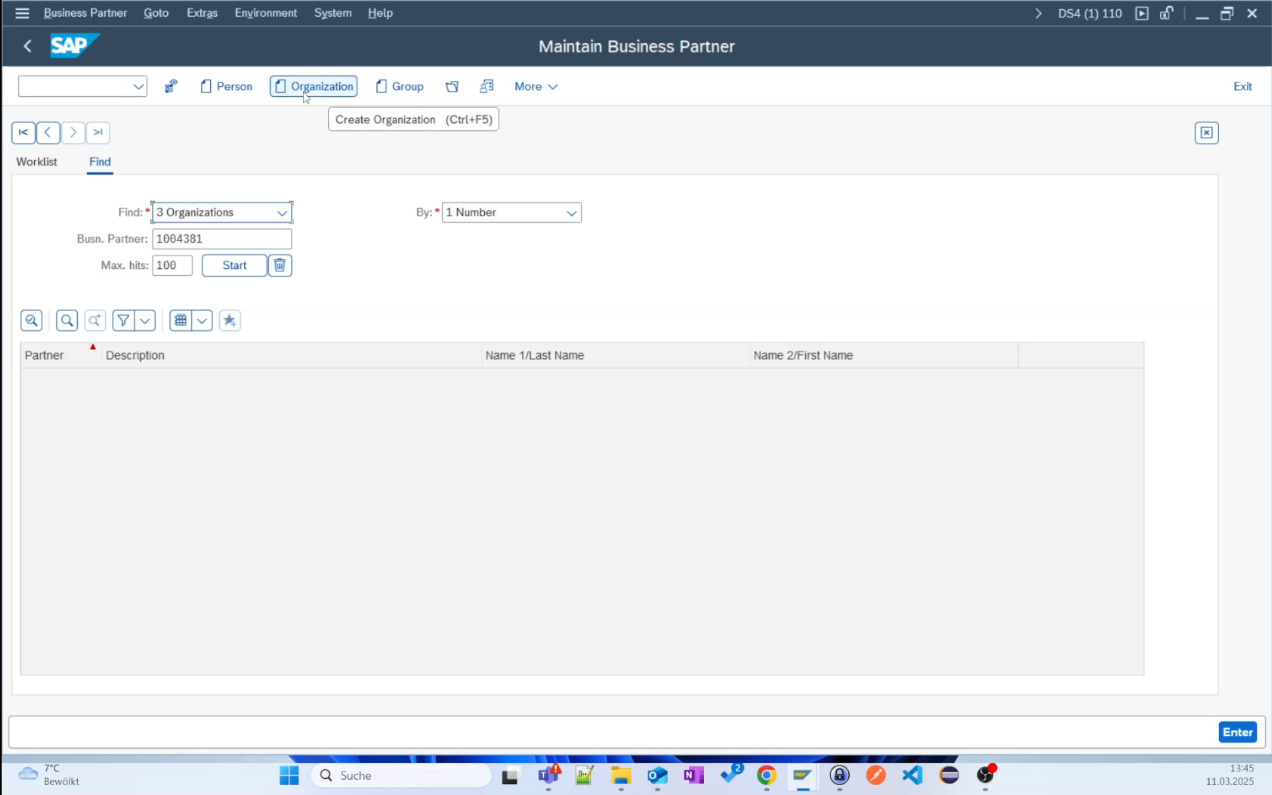
\includegraphics[width=0.8\textwidth]{Chapter5/Pictures/BP_Tcode.png}}
    \caption{Maintaining Business Partner in SAP S/4HANA}
    
    \end{figure}


    
    \item Press \textbf{Enter} to access the Business Partner maintenance screen.
\end{enumerate}



\subsubsection{Defining the Business Partner Role}
The BP framework in SAP S/4HANA allows the assignment of multiple roles to a single entity. To establish a customer relationship, the following steps are required:

\begin{enumerate}
    \item Click on the \textbf{Create Organization} or \textbf{Create Person} option, depending on the type of business partner being created.
    \item In the role selection dropdown, choose \textbf{Customer} to define the BP as a customer.
\end{enumerate}


    \begin{figure}[H]
    \centering
    \fbox{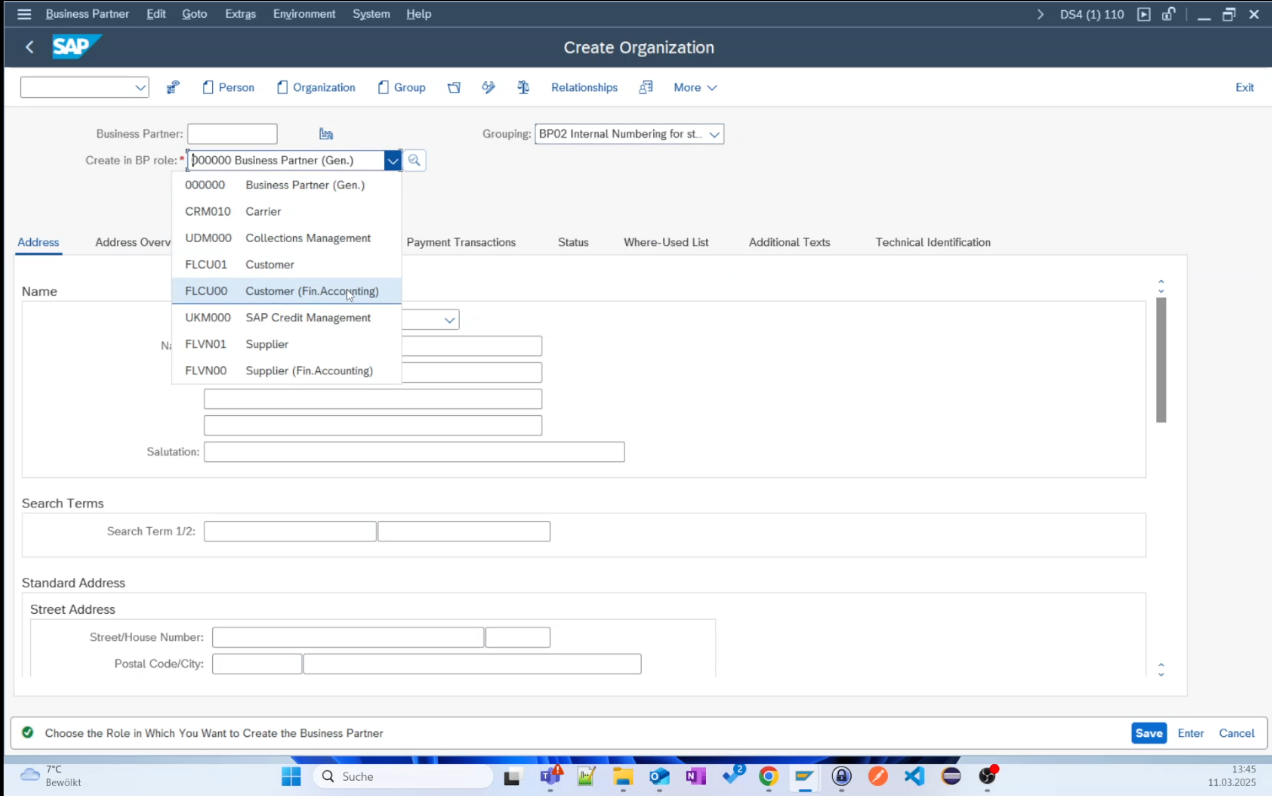
\includegraphics[width=0.8\textwidth]{Chapter5/Pictures/BP_Role.png}}
    \caption{Creating a Business Partner in SAP S/4HANA}
    
    \end{figure}

\subsubsection{Entering Business Partner Details}
After selecting the appropriate role, the system prompts the user to enter essential master data fields. These fields ensure the accurate classification and identification of the BP within SAP S/4HANA. The key required fields include:

\begin{itemize}
    \item \textbf{General Data:} Name, Address, Country, and Communication Details (e.g., Email, Phone).
    \item \textbf{Company Code Data:} Reconciliation Account and Payment Terms.
    \item \textbf{Sales and Distribution Data:} Sales Organization, Distribution Channel, Division, and Pricing Conditions.
\end{itemize}

Once all the required fields are populated, the BP record is saved and a unique Business Partner ID is generated. This ID serves as a reference for further processing and integration.


    \begin{figure}[H]
    \centering
    \fbox{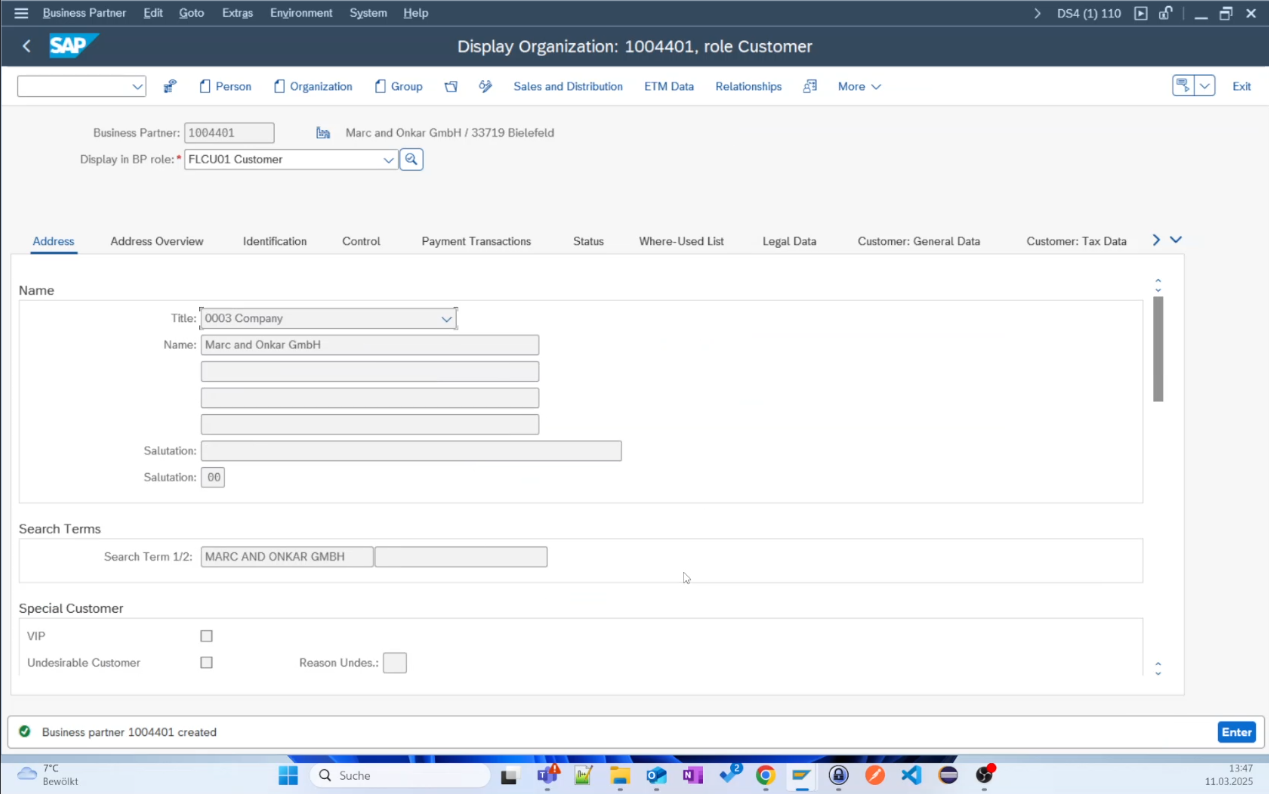
\includegraphics[width=0.8\textwidth]{Chapter5/Pictures/BP_generated.png}}
    \caption{Displaying Business Partner in SAP S/4HANA}
    
    \end{figure}

\subsubsection{Business Partner Readiness for Integration}
With the BP successfully created, it is now available for outbound integration to Salesforce via SAP CPI. The next step involves triggering the data transfer through IDoc generation, which is covered in the subsequent section.


\subsection{Step 2: iFlow Execution in SAP CPI}

Once the Business Partner (BP) is created in SAP S/4HANA, the next step involves the execution of the integration flow (iFlow) within SAP Cloud Platform Integration (CPI) to transfer the BP data to Salesforce. The iFlow acts as a middleware process, ensuring that the data is properly mapped, transformed, and securely transmitted between SAP and Salesforce.

\subsubsection{Triggering the iFlow Execution}
The iFlow in SAP CPI can be triggered in two ways:
\begin{itemize}
    \item \textbf{Scheduled Execution:} The iFlow can be configured to run at predefined intervals, ensuring periodic synchronization between SAP S/4HANA and Salesforce.
    \item \textbf{Immediate Execution:} The iFlow can be triggered manually by deploying it within SAP CPI, initiating the data transfer in real time.
\end{itemize}

For real-time synchronization, an immediate trigger is preferred, which is initiated when the iFlow is deployed.

\subsubsection{Executing the iFlow in SAP CPI}
To execute the iFlow manually, the following steps must be performed:

\begin{enumerate}
    \item \textbf{Access SAP CPI:}
    Log in to the SAP Integration Suite via the SAP BTP cockpit.
    
    \item \textbf{Navigate to the iFlow:}
    \begin{itemize}
        \item Go to the Design workspace.
        \item Locate the integration package containing the iFlow named "Replicate Account from SAP S/4HANA to Salesforce."
    \end{itemize}
    
    \begin{figure}[H]
    \centering
    \fbox{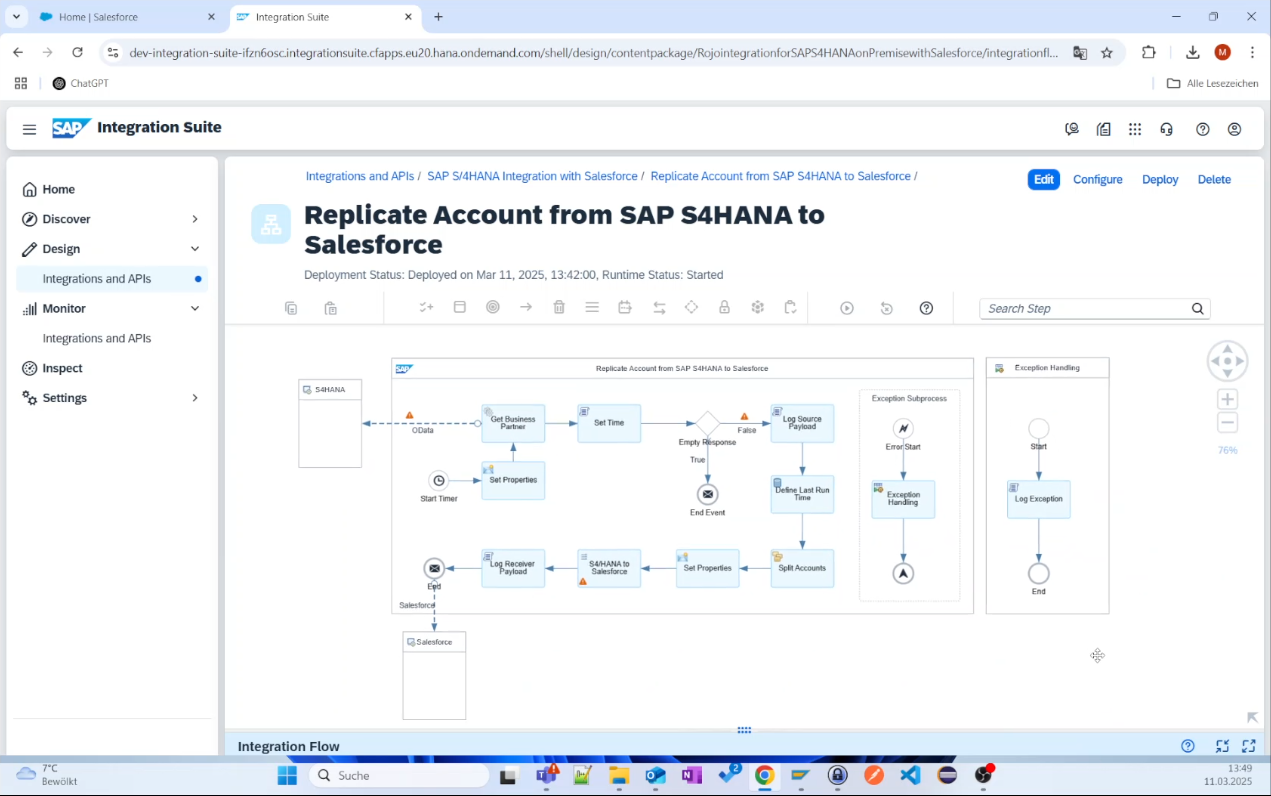
\includegraphics[width=0.8\textwidth]{Chapter5/Pictures/CPI_Locate.png}}
    \caption{Integration Flow for Replicating Accounts from SAP S/4HANA to Salesforce}
    
    \end{figure}
    
    \item \textbf{Deploy the iFlow:}
    \begin{itemize}
        \item Select the iFlow.
        \item Click on the Deploy button to initiate execution.
    \end{itemize}


    \item \textbf{Monitor the Execution Status:}
    \begin{itemize}
        \item Navigate to the Monitor tab within SAP CPI.
        \item Open Message Monitoring to check the processing status of the deployed iFlow.
    \end{itemize}

        
    \begin{figure}[H]
    \centering
    \fbox{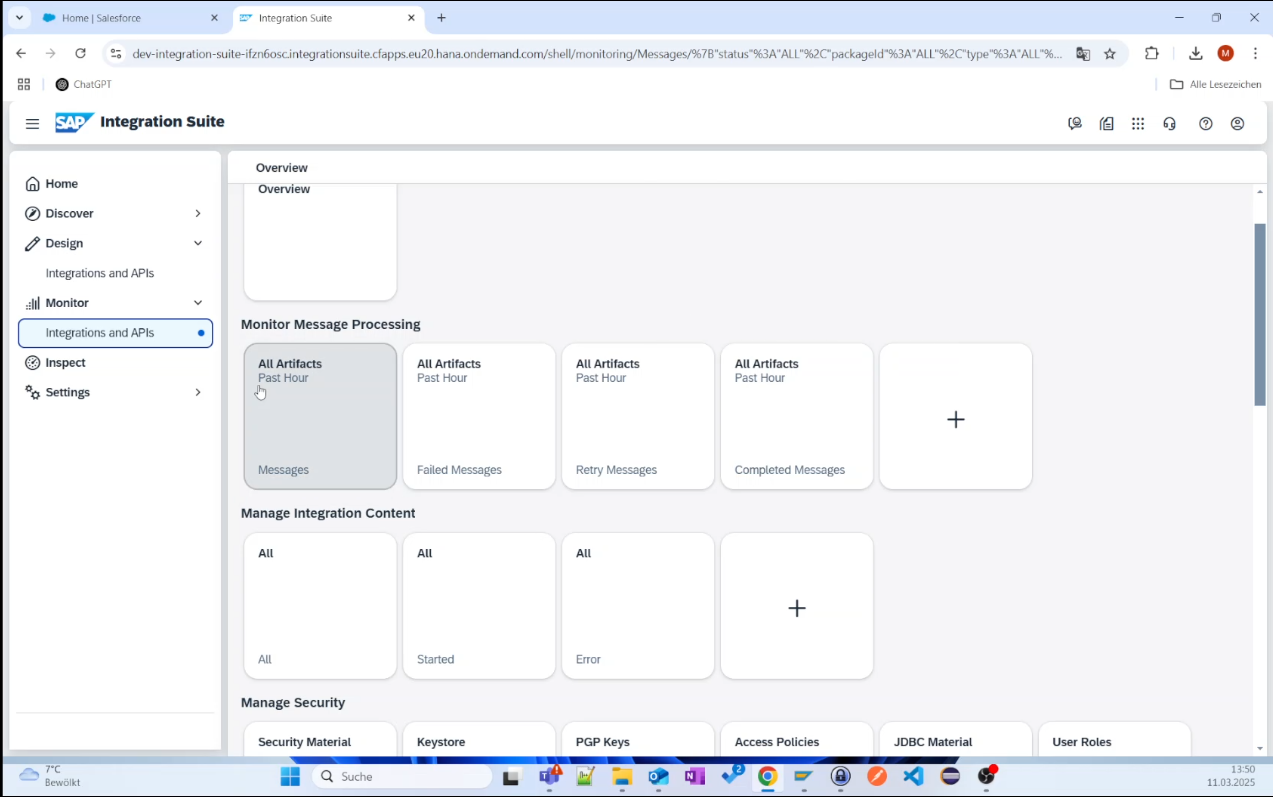
\includegraphics[width=0.8\textwidth]{Chapter5/Pictures/CPI_Mon.png}}
    \caption{Monitoring Message Processing in SAP BTP Integration Suite}
    
    \end{figure}

    \begin{figure}[H]
    \centering
    \fbox{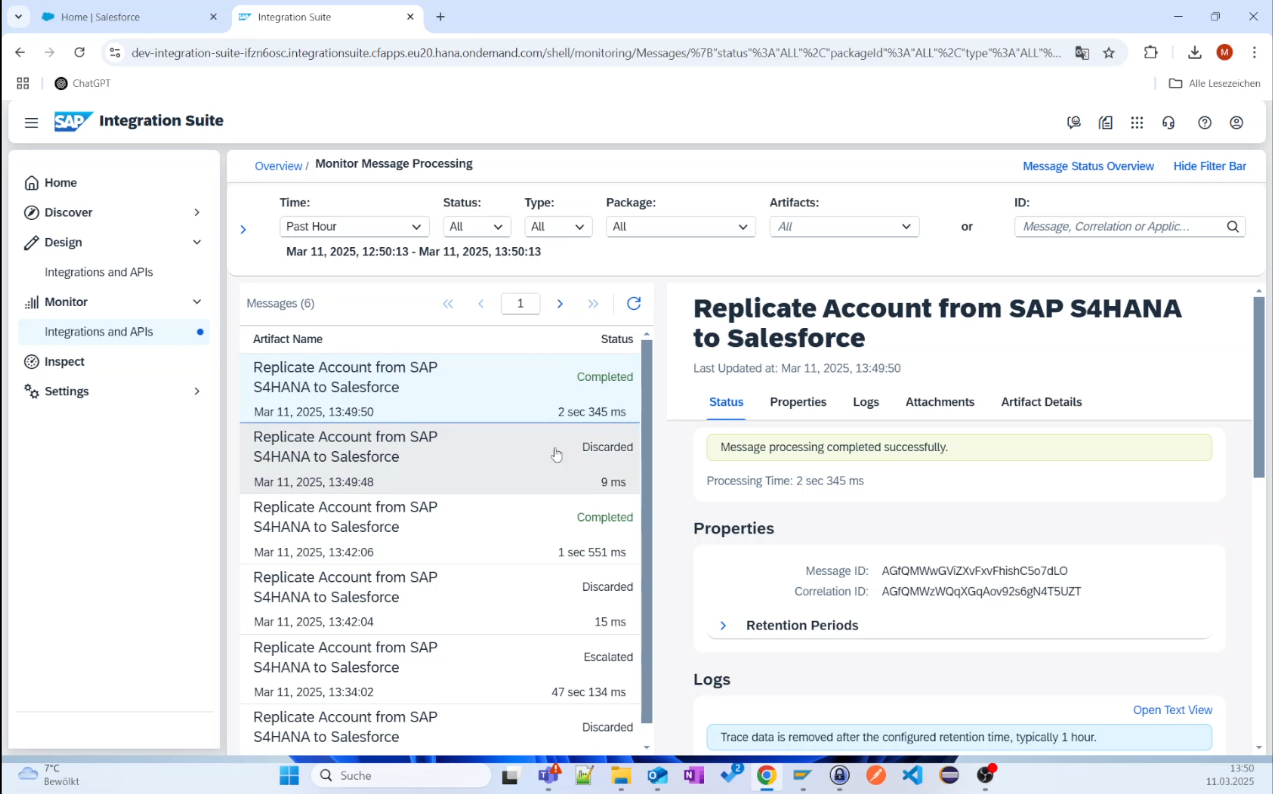
\includegraphics[width=0.8\textwidth]{Chapter5/Pictures/CPI_sucess.png}}
    \caption{Message Monitoring in SAP BTP Integration Suite}
    
    \end{figure}
    
    \item \textbf{Verify the Execution Results:}
    \begin{itemize}
        \item Look for a Success message in the message processing logs, indicating successful data transfer.
        \item Open the detailed logs to review the exact data payload transferred from SAP S/4HANA to Salesforce.
    \end{itemize}
\end{enumerate}

    \begin{figure}[H]
    \centering
    \fbox{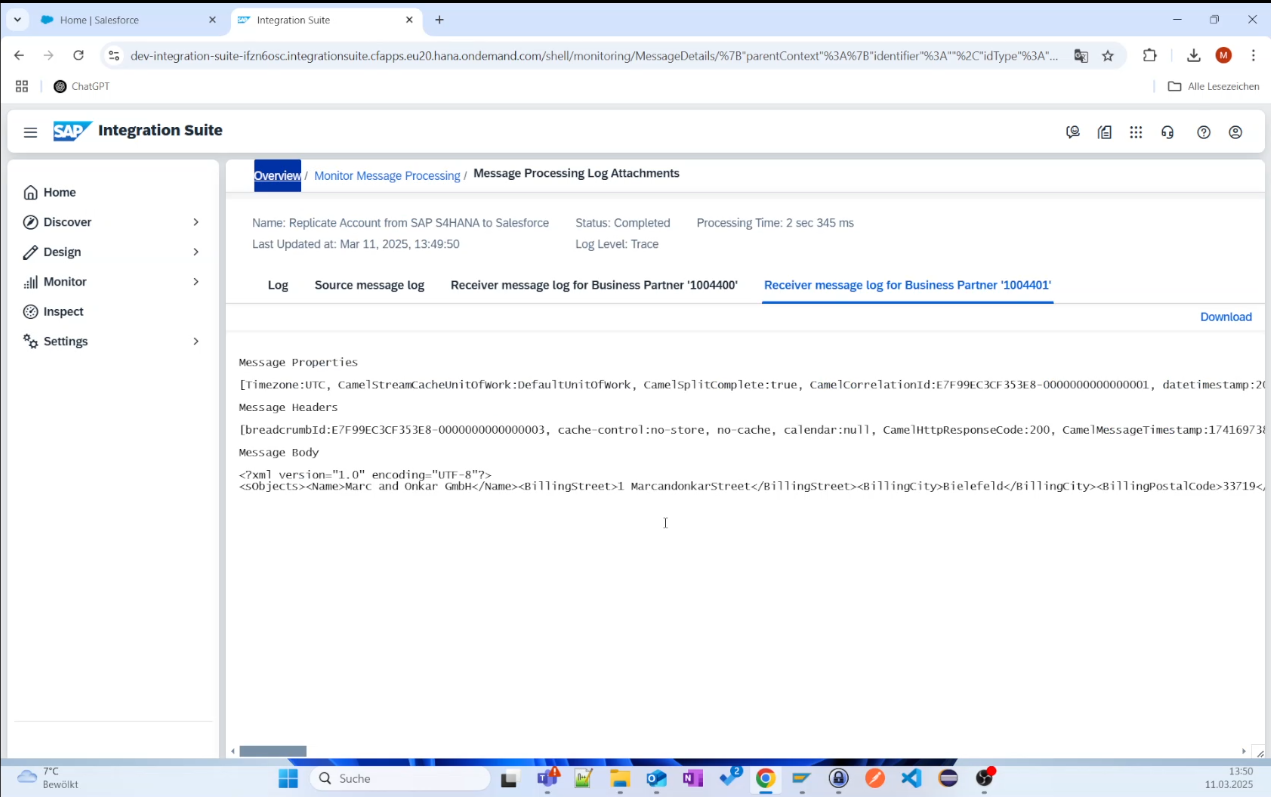
\includegraphics[width=0.8\textwidth]{Chapter5/Pictures/CPI_Verify.png}}
    \caption{Message Processing Log in SAP BTP Integration Suite}
    
    \end{figure}

This step ensures that the iFlow is successfully executed, facilitating seamless data replication from SAP S/4HANA to Salesforce. The next section explores potential error scenarios and strategies for resolving common integration challenges.

\subsection{Step 3: Login to Salesforce and Display the Transferred Business Partner as an Account}

After the successful execution of the iFlow in SAP CPI, the next step involves verifying the data transfer by logging into Salesforce and locating the Business Partner (BP) record, which is stored as an Account in Salesforce. This step ensures that the integration process has completed successfully and that the transferred data is available for business operations.

\subsubsection{Accessing Salesforce}
To verify the transferred data in Salesforce, the following steps should be performed:

\begin{enumerate}
    \item Open a web browser and navigate to the Salesforce login page at \texttt{https://login.salesforce.com}.
    \item Enter the Salesforce credentials (username and password) and click on the Login button.
    \item Once logged in, navigate to the Sales Cloud dashboard or use the global search bar to locate the transferred record.
\end{enumerate}

\subsubsection{Locating the Transferred Business Partner}
Since SAP S/4HANA's Business Partner is mapped to the Account entity in Salesforce, the transferred data can be accessed as follows:

\begin{enumerate}
    \item Click on the \textbf{Accounts} tab in the Salesforce navigation menu.

    \begin{figure}[H]
    \centering
    \fbox{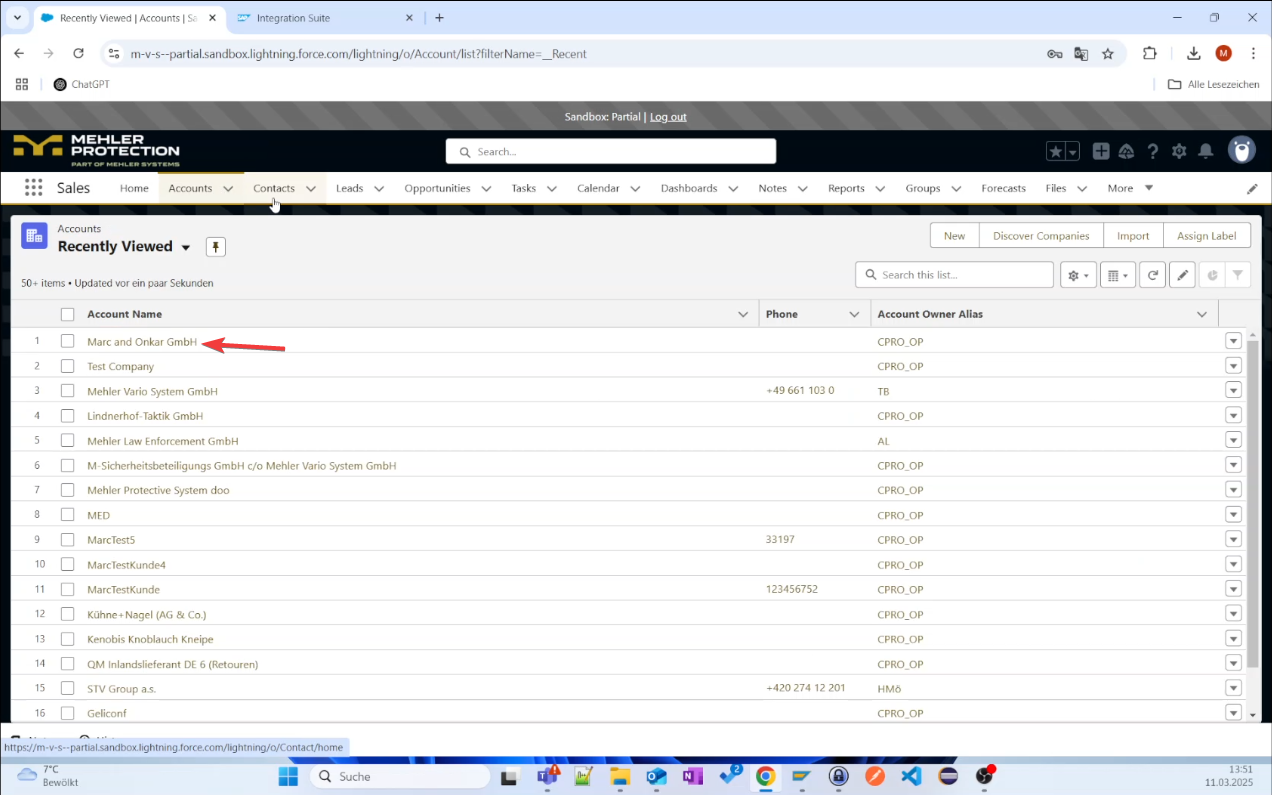
\includegraphics[width=0.8\textwidth]{Chapter5/Pictures/SF_Acc.png}}
    \caption{Salesforce Account List View}
    
    \end{figure}
    
    \item In the search bar, enter the Business Partner ID or name that was transferred from SAP S/4HANA.
    \item Click on the corresponding Account record to view its details.
\end{enumerate}

    \begin{figure}[H]
    \centering
    \fbox{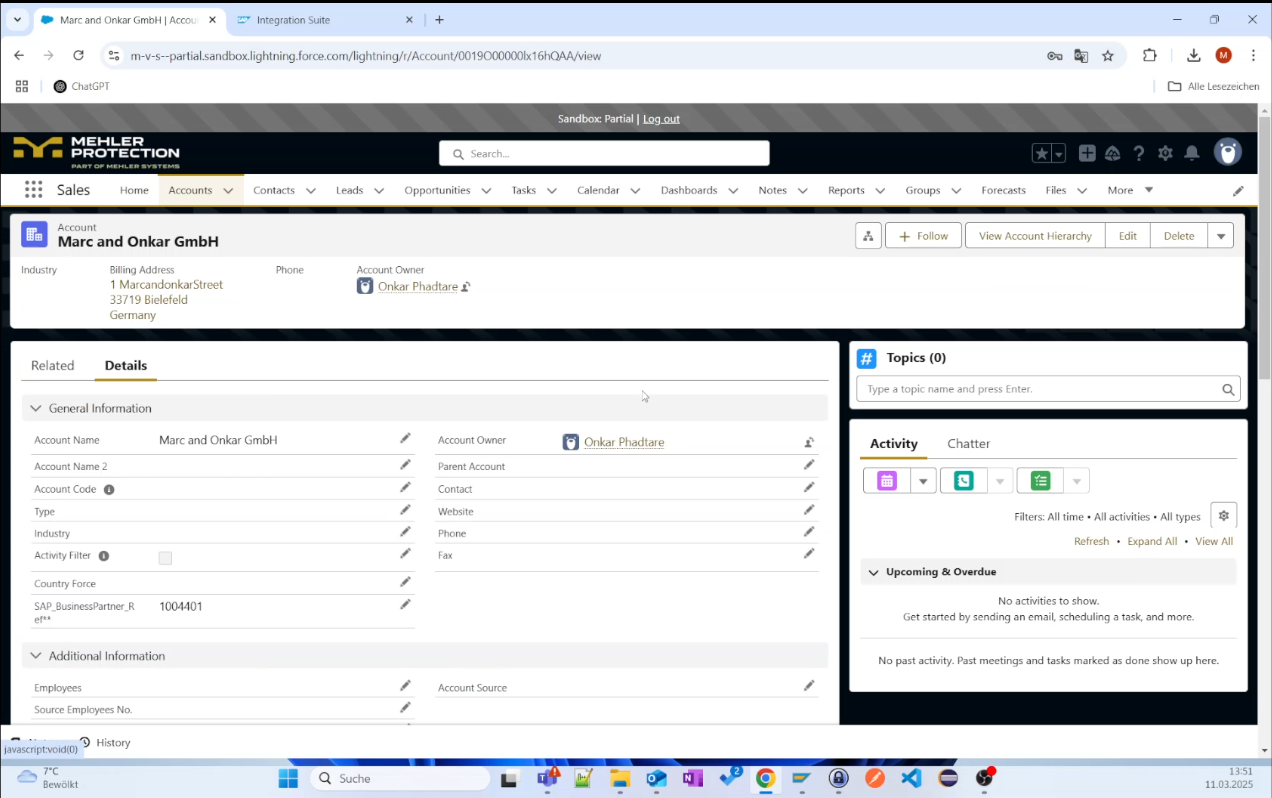
\includegraphics[width=0.8\textwidth]{Chapter5/Pictures/SF_Fields.png}}
    \caption{Salesforce Account Details Page}
    
    \end{figure}

\subsubsection{Validating Data Accuracy}
Once the Account record is opened, it is essential to verify that the data has been correctly transferred. Key fields that should be checked include:

\begin{itemize}
    \item \textbf{Account Name:} Should match the Business Partner Name in SAP S/4HANA.
    \item \textbf{Address Details:} Street, City, Postal Code, and Country should be correctly mapped.
    \item \textbf{Industry and Classification:} If applicable, ensure these attributes have been accurately assigned.
    \item \textbf{Sales Information:} Sales Group, Account Owner, and other relevant fields should be reviewed.
\end{itemize}

If any discrepancies are found, the integration logs in SAP CPI should be analyzed to determine if there were mapping errors, missing fields, or issues related to data transformation.

\subsubsection{Handling Missing or Incorrect Data}
If the Business Partner record does not appear in Salesforce, or if critical data fields are missing, the following troubleshooting steps should be performed:

\begin{itemize}
    \item Verify that the iFlow execution in SAP CPI was successful and check the message logs.
    \item Check for any API errors in Salesforce under \textit{Setup} → \textit{API Usage Logs}.
    \item Ensure that the Salesforce user account has the necessary permissions to view the Account records.
    \item Re-run the iFlow in SAP CPI and monitor if the data transfer is successful.
\end{itemize}

This step confirms the successful integration of Business Partner records from SAP S/4HANA to Salesforce. By verifying the transferred data within the Salesforce Account entity, organizations can ensure that the synchronization process maintains data integrity and supports business operations. If errors or inconsistencies arise, further analysis of the iFlow execution and data transformation logs is required to rectify the issues.



\section{Error Scenario in iFlow Execution}

While the integration of SAP S/4HANA and Salesforce through SAP CPI ensures seamless data synchronization, failures in the iFlow execution can occur due to misconfigurations, expired credentials, or network-related issues. Understanding these failure scenarios is essential for troubleshooting and improving integration reliability. 

This section examines a controlled error scenario where an expired OAuth credential is deliberately used during Business Partner (BP) creation in SAP S/4HANA. The resulting iFlow failure is analyzed through message monitoring in SAP CPI.

\subsection{Intentional Error Injection: Expired OAuth Credentials}
To demonstrate an authentication failure scenario, an expired OAuth credential is intentionally used during the execution of the iFlow. The following steps outline the controlled setup:

\begin{enumerate}
    \item \textbf{Create a Business Partner in SAP S/4HANA:}  
    A new BP is created using transaction code \texttt{BP}, following the standard process outlined in Section 5.1.
    
    \item \textbf{Modify SAP CPI Credentials:}  
    The OAuth credentials stored in SAP CPI are deliberately replaced with an expired or incorrect client secret from the Salesforce Connected App.

    \begin{figure}[H]
    \centering
    \fbox{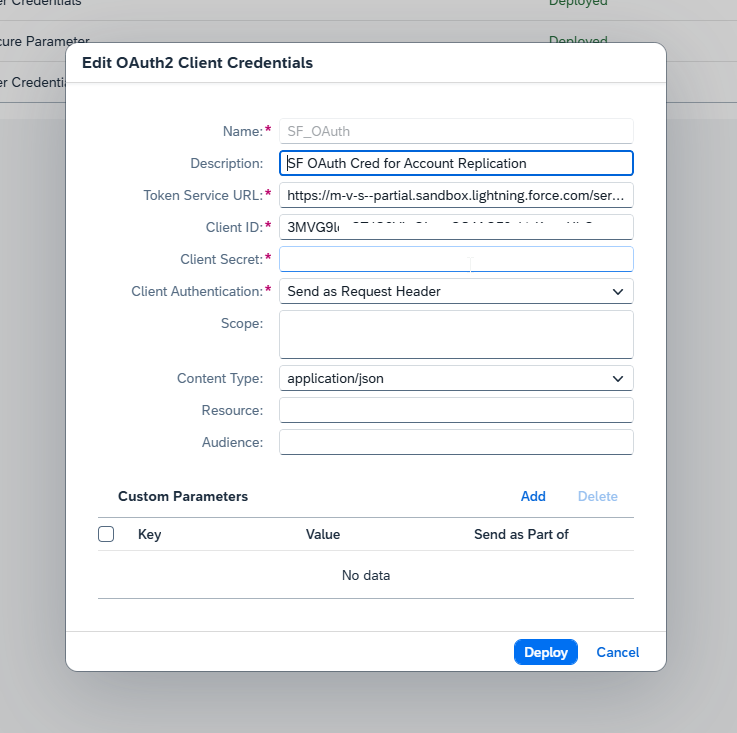
\includegraphics[width=0.8\textwidth]{Chapter5/Pictures/Fail_oauth.png}}
    \caption{OAuth2 Client Credentials Configuration in SAP Integration Suite}
    
    \end{figure}
    
    \item \textbf{Deploy the iFlow and Monitor Execution:}  
    The iFlow responsible for BP replication is deployed, initiating data transfer from SAP S/4HANA to Salesforce.
\end{enumerate}

\subsection{Failed Status in SAP CPI Monitor Tab}
After triggering the iFlow, the message monitoring dashboard in SAP CPI provides insights into the error encountered. The key observations include:

\begin{itemize}
    \item \textbf{Status:} The iFlow execution fails, displaying a "Failed" status in the Monitor tab.
    
    \begin{figure}[H]
    \centering
    \fbox{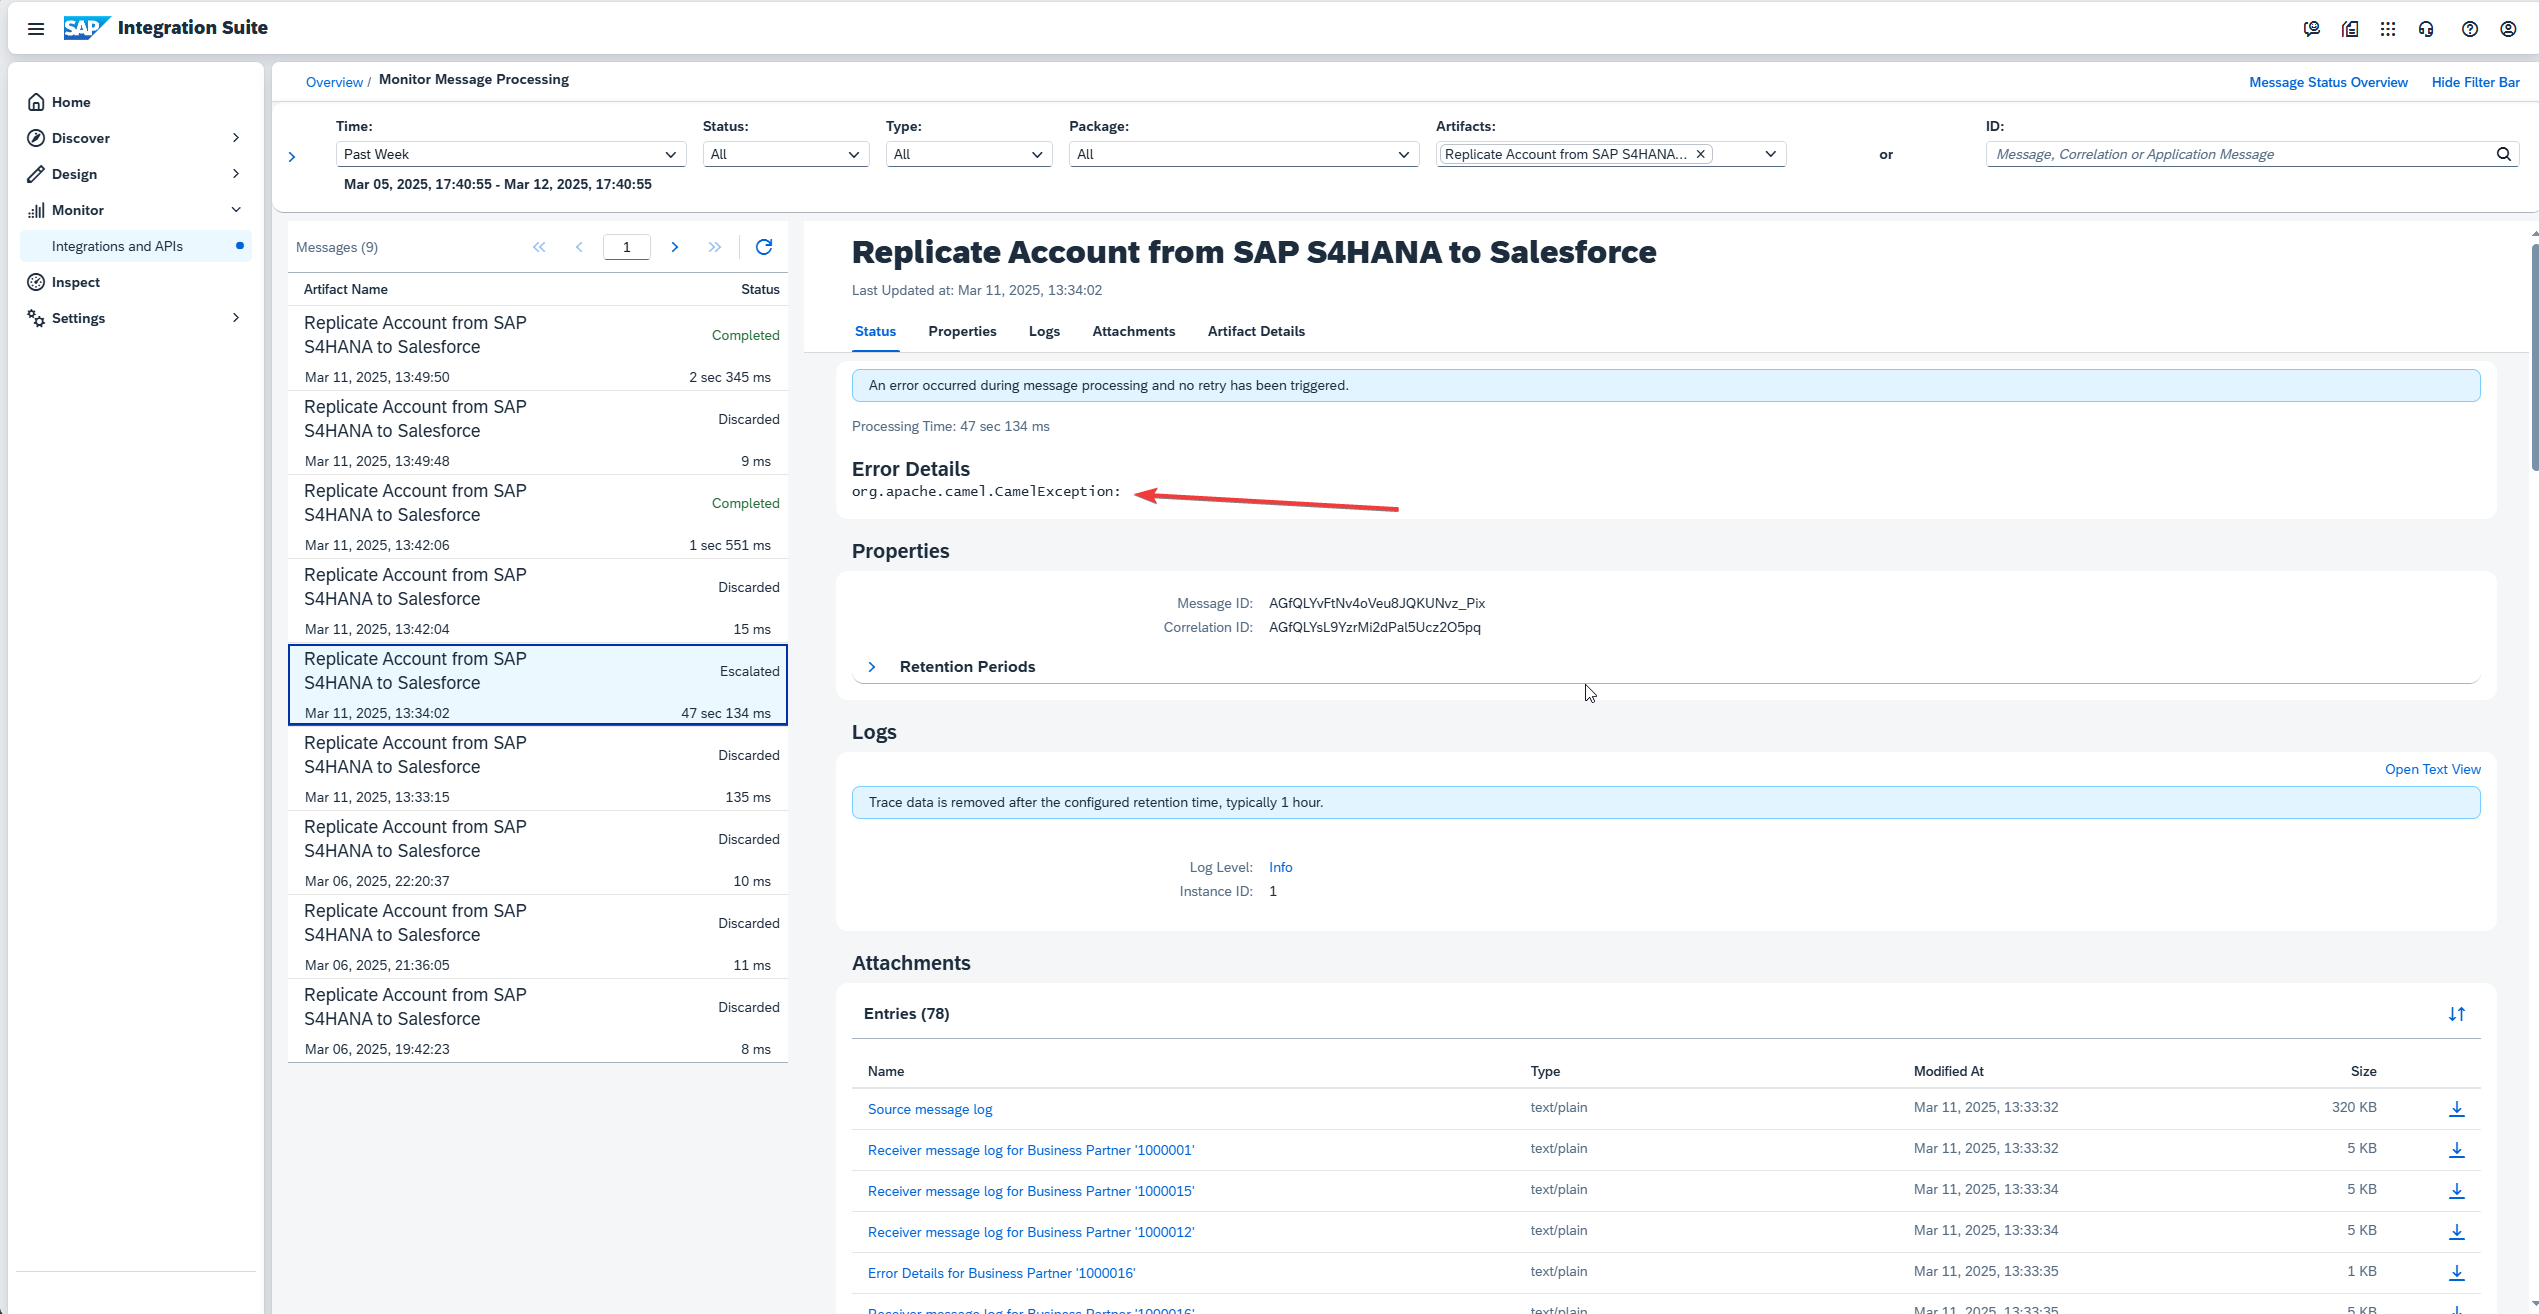
\includegraphics[width=0.8\textwidth]{Chapter5/Pictures/fail_error.png}}
    \caption{Message Processing Run in SAP BTP Integration Suite}
    
    \end{figure}
    
    \item \textbf{Error Message:} The logs indicate an authentication failure due to expired or incorrect OAuth credentials.
    \item \textbf{Timestamp and Log Details:} The failure occurs at the authentication step, preventing further processing of the BP data.
    
\end{itemize}

\subsection{Analyzing the Error Logs}
To investigate the root cause, the following log files in SAP CPI are examined:
    \begin{figure}[H]
    \centering
    \fbox{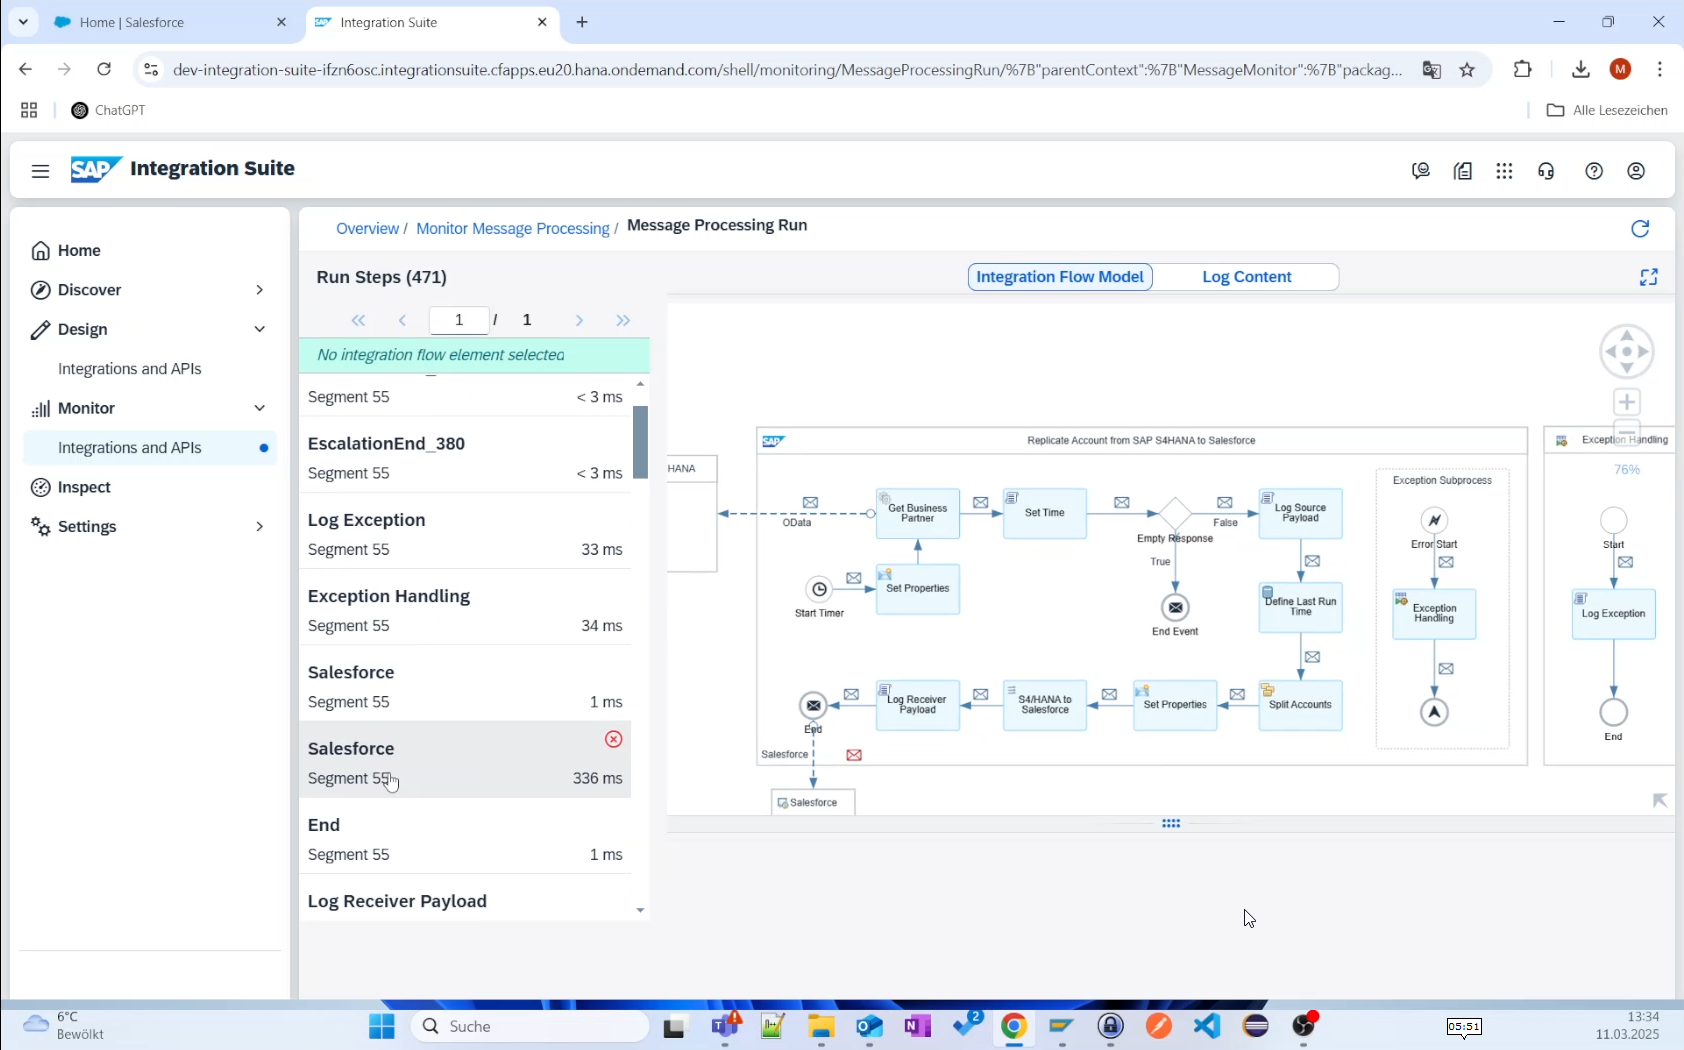
\includegraphics[width=0.8\textwidth]{Chapter5/Pictures/Fail_log.png}}
    \caption{Error Log in SAP BTP Integration Suite}
    
    \end{figure}
\begin{itemize}
    \item \textbf{Integration Message Logs:} Provide details on failed API authentication.
    \item \textbf{OAuth Token Validation:} Indicates an invalid or expired access token.
    \item \textbf{Salesforce API Logs:} Can be checked under \textit{Setup → API Usage Logs} in Salesforce to confirm rejected authentication requests.
\end{itemize}

\subsection{Corrective Measures}
To resolve this issue and ensure successful execution, the following corrective actions must be implemented:

\begin{itemize}
    \item \textbf{Regenerate OAuth Credentials:} Obtain a new access token from the Salesforce Connected App.
    \item \textbf{Update SAP CPI Credentials:} Replace the expired credentials in the security material of SAP CPI.
    \item \textbf{Re-execute the iFlow:} Once the correct credentials are in place, redeploy the iFlow and monitor execution.
\end{itemize}


This error scenario highlights the critical role of proper authentication management in SAP CPI integrations. Expired OAuth credentials can disrupt real-time data synchronization, necessitating proactive monitoring and periodic credential updates. By leveraging SAP CPI’s message monitoring and Salesforce API logs, authentication failures can be swiftly diagnosed and corrected, ensuring seamless integration between SAP S/4HANA and Salesforce.



\section{Limitations of the Current Development}

While the integration between SAP S/4HANA and Salesforce using SAP CPI enables seamless data synchronization, several limitations exist within the current development. These limitations primarily relate to field mapping complexities, inadequate error messaging, and restricted access to trial environments. Understanding these challenges is crucial for improving the integration framework and addressing potential constraints in future implementations.

\subsection{Mapping Complexity in iFlow Development}
One of the significant challenges in the current integration setup is the extensive field mapping required between SAP S/4HANA and Salesforce. Due to differences in data structures and field names between the two systems, each data element must be carefully mapped to ensure successful data transformation and transfer.

    \begin{figure}[H]
    \centering
    \fbox{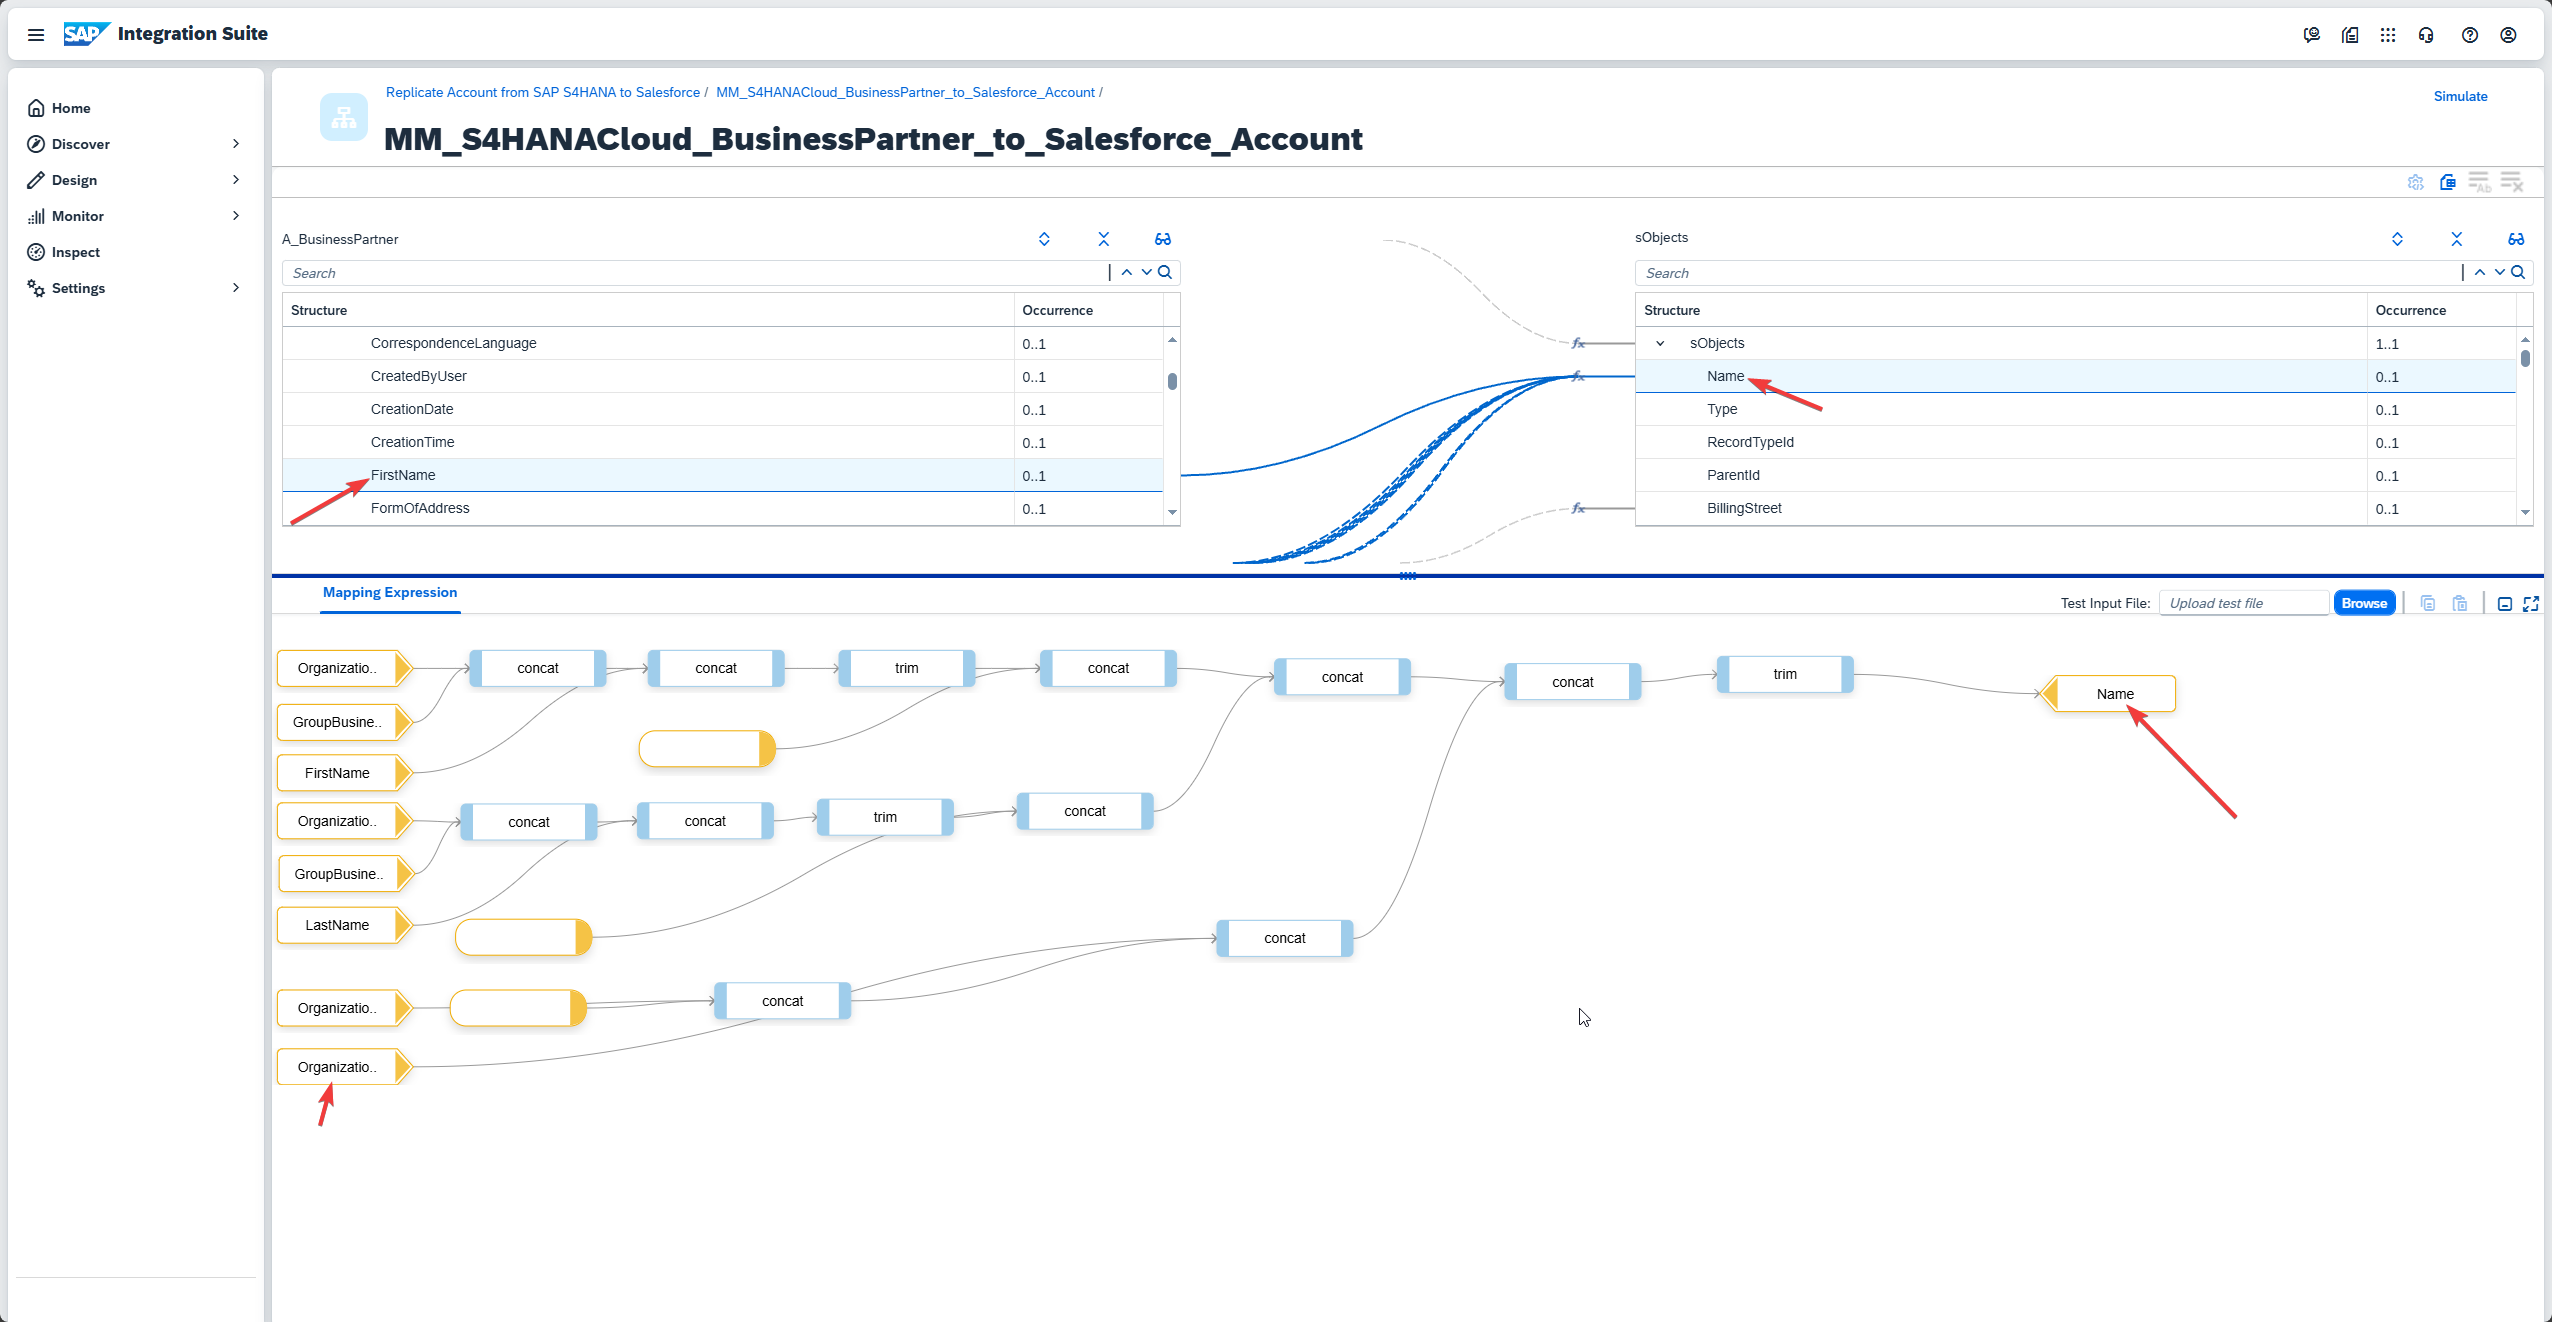
\includegraphics[width=0.8\textwidth]{Chapter5/Pictures/Map_comp.png}}
    \caption{Mapping Configuration in SAP BTP Integration Suite}
    
    \end{figure}

For example, SAP S/4HANA stores business partner names in multiple fields such as \texttt{Name1}, \texttt{Name2}, \texttt{Name3}, and \texttt{Name4}, while Salesforce represents the account name in a single field. This structural difference requires custom logic in the iFlow to concatenate and properly format the name fields before transferring the data to Salesforce. A screenshot illustrating this mapping challenge is provided below.



Such discrepancies necessitate additional transformation logic, increasing the complexity of iFlow development. Any misalignment in these mappings can result in data loss, formatting issues, or incorrect updates in Salesforce. Future improvements could focus on predefined mapping templates or automated field transformations to minimize manual effort.

\subsection{Limited Error Message Clarity}
Another critical limitation in the current development is the lack of detailed and actionable error messages in SAP CPI logs. The system often returns generic error responses, making it difficult to pinpoint the exact cause of failure.

A practical example of this issue was encountered in Section 5.2, where expired OAuth credentials were deliberately used to simulate an authentication failure. Instead of a clear authentication error message, SAP CPI returned a vague error log entry:

\begin{quote}
\texttt{Error Details org.apache.camel.CamelException:}
\end{quote}

Such non-descriptive error messages hinder troubleshooting and increase the time required for debugging. Developers must manually investigate multiple log files, cross-check API responses, and perform trial-and-error debugging to identify root causes. A potential improvement would be enhancing error verbosity in SAP CPI by enabling detailed logging or implementing structured error-handling mechanisms.

\subsection{Trial Account Restrictions and Licensing Issues}
A significant limitation in adopting this integration framework is the lack of access to the SAP CPI Integration Suite in trial accounts. Currently, SAP restricts trial users from connecting SAP S/4HANA with external applications via CPI. This creates several challenges:

\begin{itemize}
    \item Organizations must purchase a licensed SAP CPI instance before testing whether the solution fits their business needs.
    \item Without a trial version, developers cannot validate their integration scenarios without financial investment.
    \item Users exploring SAP CPI for learning or proof-of-concept purposes are unable to perform real-world testing.
\end{itemize}

The absence of trial access significantly impacts small businesses or teams evaluating SAP solutions, as they must commit to licensing costs upfront. A potential resolution could be providing limited trial access with connectivity to sandbox environments, allowing users to experiment with CPI before making financial commitments.

The current development of SAP CPI integration with Salesforce presents key challenges in field mapping, error handling, and licensing restrictions. Addressing these limitations requires enhanced mapping automation, more detailed error logs, and improved access to trial environments. Future enhancements in these areas would make the integration process more efficient and accessible for businesses looking to implement seamless data synchronization between SAP S/4HANA and Salesforce.


%=== END OF CHAPTER FIVE ===
\newpage

%=== CHAPTER SIX (6) ===
%=== Conclusion and Recommendations ===

\chapter{Conclusion}


\section{ERP-CRM Integration: Challenges and Solutions}

The integration ofERP andCRM systems, particularly between SAP S/4HANA and Salesforce, represents a critical challenge for modern enterprises aiming to streamline business processes, enhance operational efficiency, and improve customer satisfaction. This thesis explores the technical and operational challenges associated with ERP-CRM integration, focusing on the use of SAP BTP (BTP) Integration Suite as a middleware solution to facilitate seamless DS. The findings are summarized below, highlighting key insights, challenges, and outcomes.

\subsection{The Necessity of ERP-CRM Integration}
Integrating ERP and CRM systems creates a unified data ecosystem. ERP systems, such as SAP S/4HANA, manage internal business processes like finance, supply chain, and inventory management, while CRM systems like Salesforce focus on customer-facing activities such as sales, marketing, and customer service. Operating these systems in isolation leads to data silos, inconsistent records, and inefficient workflows. 

The integration of SAP S/4HANA and Salesforce enables real-time DS, eliminates manual data entry, and provides a 360-degree customer view. Sales representatives gain access to up-to-date customer data, including order details and account updates, enhancing their ability to respond promptly and improve overall sales efficiency.

\subsection{Challenges in ERP-CRM Integration}
Several technical and operational challenges arise in integrating SAP S/4HANA and Salesforce:

\subsubsection{DS and Consistency}
Ensuring consistent data across both systems is a primary challenge. Differences in data structures, formats, and identifiers can create discrepancies in customer records, order details, and sales forecasts. Middleware solutions like SAP BTP Integration Suite address these challenges by providing pre-built connectors, data transformation tools, and real-time synchronization capabilities.

\subsubsection{Technical Barriers}
Integration is complicated by differences in API architectures, security protocols, and data models. SAP S/4HANA primarily uses OData and SOAP-based web services, while Salesforce relies on RESTful APIs and GraphQL. These differences create interoperability issues requiring custom API connectors and middleware solutions. SAP BTP Integration Suite bridges these gaps with pre-configured integration flows, API management tools, and error-handling mechanisms.

\subsubsection{Security and Compliance}
Ensuring data security and compliance is another critical challenge. Strong security measures such as OAuth 2.0 authentication, data encryption, and role-based access controls are required to protect sensitive customer and financial data. SAP BTP Integration Suite provides built-in security features, including encryption in transit and at rest, ensuring compliance with GDPR, SOX, and HIPAA regulations.

\subsection{The Role of SAP BTP Integration Suite}
SAP BTP Integration Suite serves as a powerful middleware solution for integrating SAP S/4HANA and Salesforce. Key features include:

\subsubsection{Pre-Built Connectors and Integration Flows}
Pre-configured integration flows (iFlows) simplify connecting SAP S/4HANA and Salesforce, reducing the need for custom development and accelerating implementation.

\subsubsection{Real-Time Data Processing}
The suite supports real-time DS, ensuring updates in SAP S/4HANA are immediately reflected in Salesforce and vice versa. This capability maintains data consistency and enables timely decision-making.

\subsubsection{Scalability and Flexibility}
SAP BTP Integration Suite scales with business growth, supporting hybrid and multi-cloud environments, enabling seamless connections between on-premise SAP S/4HANA and cloud-based Salesforce applications.

\subsubsection{Error Handling and Monitoring}
Robust error-handling mechanisms, including automatic retries, logging, and alerts, ensure integration reliability and quick issue resolution.

\subsection{Implementation and Validation}
The research includes a detailed technical implementation of SAP S/4HANA and Salesforce integration using SAP BTP Integration Suite. The implementation involves configuring integration flows, setting up authentication mechanisms, and mapping data fields.

A test scenario validated the integration, where a Business Partner in SAP S/4HANA was converted into a Salesforce Account. The results confirmed improved data accuracy, reduced manual intervention, and enhanced sales efficiency. However, some limitations were noted, including the complexity of data mapping, unclear error messages, and restrictions in trial accounts.

\subsection{Business Impact and Benefits}
The integration of SAP S/4HANA and Salesforce using SAP BTP Integration Suite provides several key benefits:

\subsubsection{Improved Productivity}
Automation reduces administrative burdens, allowing employees to focus on higher-value tasks.

\subsubsection{Enhanced Data Accuracy}
Real-time synchronization ensures consistent data across systems, improving decision-making and reporting.

\subsubsection{Better Customer Service}
A unified customer view enables quicker and more accurate responses to inquiries, enhancing customer satisfaction and loyalty.

\subsubsection{Cost Savings}
Automated processes reduce labor costs and minimize errors, improving return on investment (ROI).

\subsubsection{Increased Business Agility}
The suite's flexibility and scalability allow businesses to quickly adapt to market demands and operational requirements.

\subsection{Future Trends in ERP-CRM Integration}
Emerging trends include the use of artificial intelligence (AI) and ML for data mapping and transformation, the adoption of serverless integration solutions, and increasing regulatory compliance requirements. These advancements will further enhance the efficiency, scalability, and security of ERP-CRM integration.

In a Nutshell, The research demonstrates that integrating SAP S/4HANA and Salesforce using SAP BTP Integration Suite is a technically viable and efficient solution. The findings highlight the importance of middleware solutions in enabling seamless DS, improving operational efficiency, and enhancing customer satisfaction. This research provides a practical implementation guide for organizations aiming to integrate SAP S/4HANA and Salesforce, offering valuable insights into the technical and operational aspects of the integration process.



\section{Contribution of this Research}

This research makes several significant contributions to the field of ERP-CRM integration, particularly in the context of integrating SAP S/4HANA and Salesforce using SAP BTP (BTP) Integration Suite. The study not only addresses the technical and operational challenges of ERP-CRM integration but also provides a practical, step-by-step guide for implementing a middleware-based integration solution. Below are the key contributions of this research:

\subsection{Addressing the Gap in Practical Implementation Research}
One of the primary contributions of this research is its focus on the practical implementation of ERP-CRM integration. While there is a wealth of theoretical and strategic literature on ERP-CRM integration, there is a notable lack of detailed, hands-on guides that provide step-by-step instructions for implementing such integrations. This thesis fills that gap by offering a comprehensive, technical implementation guide for integrating SAP S/4HANA and Salesforce using SAP BTP Integration Suite. The research provides detailed instructions on configuring integration flows (iFlows), setting up authentication mechanisms, mapping data fields, and handling errors, making it a valuable resource for IT professionals and developers tasked with implementing similar integrations.

\subsection{Demonstrating the Effectiveness of SAP BTP Integration Suite}
This research contributes to the growing body of knowledge on SAP BTP Integration Suite by demonstrating its effectiveness as a middleware solution for ERP-CRM integration. The study showcases how SAP BTP Integration Suite can be used to overcome the technical challenges of integrating SAP S/4HANA and Salesforce, such as differences in API architectures, data structures, and security protocols. By providing a real-world implementation scenario, the research validates the capabilities of SAP BTP Integration Suite, including its pre-built connectors, real-time data processing, and error-handling mechanisms. This contribution is particularly valuable for organizations considering SAP BTP as a middleware solution for their integration needs.

\subsection{Providing Insights into DS and Consistency}
DS and consistency are critical challenges in ERP-CRM integration, and this research provides valuable insights into how these challenges can be addressed using middleware solutions. The study highlights the importance of real-time DS in maintaining data consistency across SAP S/4HANA and Salesforce. It also explores the role of data mapping and transformation in ensuring that data from one system is accurately reflected in the other. By providing a detailed analysis of these issues and demonstrating how they can be resolved using SAP BTP Integration Suite, the research contributes to a deeper understanding of DS in ERP-CRM integration.

\subsection{Highlighting the Importance of Security and Compliance}
Security and compliance are major concerns in ERP-CRM integration, particularly when sensitive customer and financial data is involved. This research contributes to the field by highlighting the importance of robust security measures, such as OAuth 2.0 authentication, data encryption, and role-based access controls, in ensuring the security and compliance of integrated systems. The study demonstrates how SAP BTP Integration Suite provides built-in security features that help organizations comply with regulatory requirements such as GDPR, SOX, and HIPAA. This contribution is particularly relevant for organizations operating in highly regulated industries, where data security and compliance are paramount.

\subsection{ Offering a Framework for Future Research}
This research provides a framework for future studies on ERP-CRM integration by identifying key challenges, best practices, and future trends. The study highlights the potential of emerging technologies, such as artificial intelligence (AI) and ML, in enhancing data mapping and transformation processes. It also explores the role of serverless integration solutions in improving scalability and reducing infrastructure overhead. By offering a comprehensive analysis of these trends, the research provides a foundation for future studies that seek to explore new technologies and methodologies for ERP-CRM integration.

\subsection{Enhancing Business Efficiency and Customer Satisfaction}
One of the most significant contributions of this research is its focus on the business impact of ERP-CRM integration. The study demonstrates how integrating SAP S/4HANA and Salesforce can improve business efficiency, enhance customer satisfaction, and drive revenue growth. By providing a unified view of customer data, the integration enables organizations to respond more quickly and accurately to customer inquiries, which enhances customer satisfaction and loyalty. The research also highlights the cost savings and productivity gains that can be achieved through automation and real-time DS. These insights are valuable for business leaders and decision-makers who are considering ERP-CRM integration as a strategic initiative.

\subsection{Providing a Repeatable Framework for Other Enterprises}
This research provides a repeatable framework for integrating SAP S/4HANA and Salesforce using SAP BTP Integration Suite, which can be adapted by other enterprises facing similar integration challenges. The study offers a detailed, step-by-step guide that covers all aspects of the integration process, from system configuration and data mapping to error handling and monitoring. This framework can serve as a blueprint for other organizations looking to implement similar integrations, reducing the time and effort required for implementation and increasing the likelihood of success.

\subsection{Contributing to the Academic Literature on ERP-CRM Integration}
Finally, this research contributes to the academic literature on ERP-CRM integration by providing a comprehensive analysis of the challenges, best practices, and future trends in this field. The study synthesizes knowledge from academic research, industry reports, and case studies to provide a structured understanding of ERP-CRM integration. By addressing the gap in practical implementation research and offering a detailed technical guide, the research adds to the growing body of knowledge on ERP-CRM integration and provides a valuable resource for academics, researchers, and practitioners.

In conclusion, this research makes several important contributions to the field of ERP-CRM integration, particularly in the context of integrating SAP S/4HANA and Salesforce using SAP BTP Integration Suite. The study provides a practical, hands-on guide for implementing ERP-CRM integration, demonstrates the effectiveness of SAP BTP Integration Suite, and offers valuable insights into DS, security, and compliance. The research also provides a framework for future studies and contributes to the academic literature on ERP-CRM integration, making it a valuable resource for IT professionals, business leaders, and researchers alike.

\section{6.3 Limitations of the Study}

While this research provides valuable insights into the integration of SAP S/4HANA and Salesforce using SAP BTP Integration Suite, it is important to acknowledge the limitations of the study. These limitations highlight areas where the research could be improved or expanded in future studies.

\subsection{Scope of Integration Scenarios}
One of the primary limitations of this research is its focus on a specific integration scenario: the synchronization of Business Partner data from SAP S/4HANA to Salesforce. While this scenario is representative of common ERP-CRM integration challenges, it does not cover other integration scenarios, such as sales order processing, inventory management, or financial DS. Future studies could explore a broader range of integration scenarios to provide a more comprehensive understanding of ERP-CRM integration.

\subsection{Complexity of Data Mapping}
The research highlights the complexity of data mapping between SAP S/4HANA and Salesforce due to differences in data structures, formats, and identifiers. While SAP BTP Integration Suite provides tools for data transformation, the process of mapping fields between the two systems remains time-consuming and requires significant manual effort. Future research could explore the use of artificial intelligence (AI) and ML to automate data mapping and reduce the complexity of integration.

\subsection{Limited Error Message Clarity}
Another limitation of this research is the lack of detailed and actionable error messages in SAP BTP Integration Suite. During the implementation process, generic error messages made it difficult to diagnose and resolve issues quickly. Future studies could focus on improving error-handling mechanisms in middleware solutions, such as SAP BTP Integration Suite, by providing more detailed error logs and actionable insights.

\subsection{Trial Account Restrictions}
The research was conducted using trial accounts for SAP BTP Integration Suite and Salesforce, which imposed certain restrictions on functionality and scalability. For example, trial accounts often have limitations on data volume, API calls, and integration capabilities, which may not reflect real-world scenarios. Future research could be conducted using full-featured, enterprise-grade accounts to validate the findings in a more realistic environment.

\subsection{Industry-Specific Considerations}
This research focuses on a general integration scenario and does not address industry-specific requirements or challenges. For example, industries such as healthcare, finance, and manufacturing may have unique data structures, compliance requirements, and integration needs that were not considered in this study. Future research could explore ERP-CRM integration in specific industries to provide tailored solutions and insights.

\subsection{Scalability and Performance}
While the research demonstrates the feasibility of integrating SAP S/4HANA and Salesforce using SAP BTP Integration Suite, it does not extensively test the scalability and performance of the integration in large-scale enterprise environments. Future studies could evaluate the performance of the integration under high data volumes, complex workflows, and multi-tenant architectures to ensure its suitability for large organizations.

By addressing these limitations, future research can build on the findings of this study and provide more comprehensive, scalable, and industry-specific solutions for ERP-CRM integration.


\section{Future Research Directions}

The findings of this research demonstrate the feasibility and effectiveness of integrating SAP S/4HANA and Salesforce using the SAP BTP Integration Suite as a middleware solution. However, the dynamic and evolving nature of enterprise systems integration presents multiple avenues for further study. This section outlines key research directions that could build upon the insights gained in this study, offering practical, technical, and strategic advancements in ERP-CRM integration.

\subsection{Expansion of Integration Scenarios Beyond Business Partners}
This study primarily focused on business partner synchronization and account updates. Future research could broaden the scope by incorporating additional integration scenarios that align with core enterprise functions, such as:

\begin{itemize}
    \item Sales order processing: Automating order creation in SAP S/4HANA based on Salesforce opportunities, ensuring end-to-end traceability from lead generation to invoice generation.
    \item Inventory and supply chain synchronization: Enhancing real-time updates for stock levels, procurement processes, and supply chain logistics to reduce discrepancies between customer demand and warehouse availability.
    \item Financial and billing data integration: Bridging financial transactions between ERP and CRM systems to enable seamless invoicing, revenue recognition, and payment reconciliation.
    \item Service and warranty management: Extending integration to post-sales support by ensuring synchronized customer service records across both systems.
\end{itemize}

Future research in these areas would require an in-depth examination of the data structures, business rules, and transaction workflows necessary for extending middleware-based ERP-CRM integration to these complex business processes.

\subsection{Leveraging Artificial Intelligence and ML for Intelligent Data Mapping}
One of the major challenges in ERP-CRM integration is the heterogeneity of data models between SAP S/4HANA and Salesforce. Future studies could explore the application of artificial intelligence (AI) and ML techniques to:

\begin{itemize}
    \item Automate data mapping and transformation: Develop AI-powered algorithms capable of detecting data similarities and suggesting mappings based on historical integration patterns.
    \item Predictive DS: Utilize ML models to forecast changes in customer accounts, sales orders, and supply chain data, ensuring proactive synchronization rather than reactive updates.
    \item Anomaly detection and error prevention: AI-driven validation mechanisms could identify inconsistencies in synchronized data, preventing erroneous transactions and minimizing reconciliation efforts.
\end{itemize}

\subsection{Enhancement of Error Handling and Exception Management}
Error handling remains a significant challenge in middleware-based integration, particularly in systems as complex as SAP and Salesforce. Future research could focus on:

\begin{itemize}
    \item Developing advanced error categorization models: Establishing a taxonomy of common integration errors to enable more granular troubleshooting.
    \item Self-healing mechanisms for DS failures: Implementing machine-learning-based error correction algorithms that detect and automatically retry failed transactions with intelligent adjustments.
    \item Improving API error messaging: Enhancing the clarity and granularity of error messages by translating cryptic system logs into actionable insights for system administrators.
\end{itemize}

\subsection{Industry-Specific ERP-CRM Integration Frameworks}
Enterprise integration requirements vary significantly across industries. Future research could explore:

\begin{itemize}
    \item Manufacturing and supply chain: Studying how ERP-CRM integration can optimize procurement, order fulfillment, and supplier relationship management.
    \item Retail and e-commerce: Investigating how real-time DS can improve customer engagement, personalization, and omnichannel sales strategies.
    \item Healthcare and pharmaceuticals: Examining compliance requirements, such as HIPAA and GDPR, to ensure secure patient DS between ERP and CRM systems.
    \item Financial services: Researching how financial institutions can benefit from automated customer risk assessment and real-time transaction tracking.
\end{itemize}

\subsection{Scalability and Performance Optimization in Large-Scale Deployments}
As enterprises grow, the performance and scalability of integration solutions become critical. While SAP BTP offers robust scalability features, further research could evaluate:

\begin{itemize}
    \item Impact of high-volume data transfers on system performance: Measuring the latency and efficiency of DS in high-transaction environments.
    \item Optimizing middleware orchestration for parallel processing: Investigating techniques such as multi-threading, caching, and distributed computing to enhance data processing speeds.
    \item Comparative analysis of integration performance across cloud and on-premise deployments: Understanding whether hybrid cloud models provide better performance than fully on-premise or cloud-based deployments.
\end{itemize}

\subsection{Strengthening Security, Compliance, and Data Governance}
Security and compliance remain paramount concerns in ERP-CRM integrations, particularly when dealing with sensitive customer and financial data. Future studies could explore:

\begin{itemize}
    \item Advanced data encryption and privacy mechanisms: Investigating cryptographic approaches for safeguarding data in transit and at rest.
    \item Role-based access control (RBAC) enhancements: Developing more sophisticated access control models that dynamically adjust based on user behavior and risk assessment.
    \item Automating compliance audits: Exploring how AI-driven compliance monitoring tools could detect and flag potential violations of GDPR, SOX, and HIPAA regulations.
\end{itemize}

\subsection{User Adoption, Change Management, and Organizational Impact}
Even the most technically sophisticated integration solutions may fail if they are not effectively adopted by end users. Future research should investigate:

\begin{itemize}
    \item Employee training and onboarding models: Developing structured training programs to help employees adapt to ERP-CRM integration changes.
    \item Measuring user satisfaction and efficiency gains: Conducting empirical studies to assess whether integration solutions genuinely improve operational efficiency and customer engagement.
    \item Change management strategies for ERP-CRM implementations: Identifying best practices for minimizing resistance and ensuring smooth transitions during integration rollouts.
\end{itemize}

\subsection{Exploring Emerging Integration Technologies}
As enterprise technology evolves, new paradigms for ERP-CRM integration continue to emerge. Future studies could investigate:

\begin{itemize}
    \item Serverless integration approaches: Exploring event-driven architectures that eliminate the need for dedicated middleware infrastructure.
    \item Blockchain for data integrity: Evaluating blockchain technology as a potential decentralized ledger for tracking changes in ERP and CRM records.
    \item Edge computing for low-latency synchronization: Researching the feasibility of processing integration logic at the edge to reduce dependency on cloud computing.
\end{itemize}

This study has provided a foundation for understanding and implementing SAP S/4HANA-Salesforce integration using SAP BTP Integration Suite. However, as enterprise integration challenges evolve, further research is necessary to expand the scope of integration scenarios, incorporate AI-driven automation, enhance security, improve scalability, and address industry-specific needs. Future studies in these areas will pave the way for next-generation enterprise integrations that are more intelligent, resilient, and business-centric.


%=== END OF CHAPTER SIX ===
\newpage

%==== ENDING PART ===

\bibliographystyle{unsrt}
\bibliography{Ref/References}

%=== APPENDIX ===
%=== APPENDIX ===

\chapter{Appendix}

\section{Appendix A: API Configuration for Integration}

This appendix provides detailed API configurations and field mappings necessary for integrating SAP S/4HANA with Salesforce. It includes endpoint specifications, sample API requests, authentication mechanisms, and field-level transformations to ensure seamless data synchronization.

\paragraph{}
\textbf{S4 HANA Configuration}

\begin{figure}[h]
    \centering
     \fbox{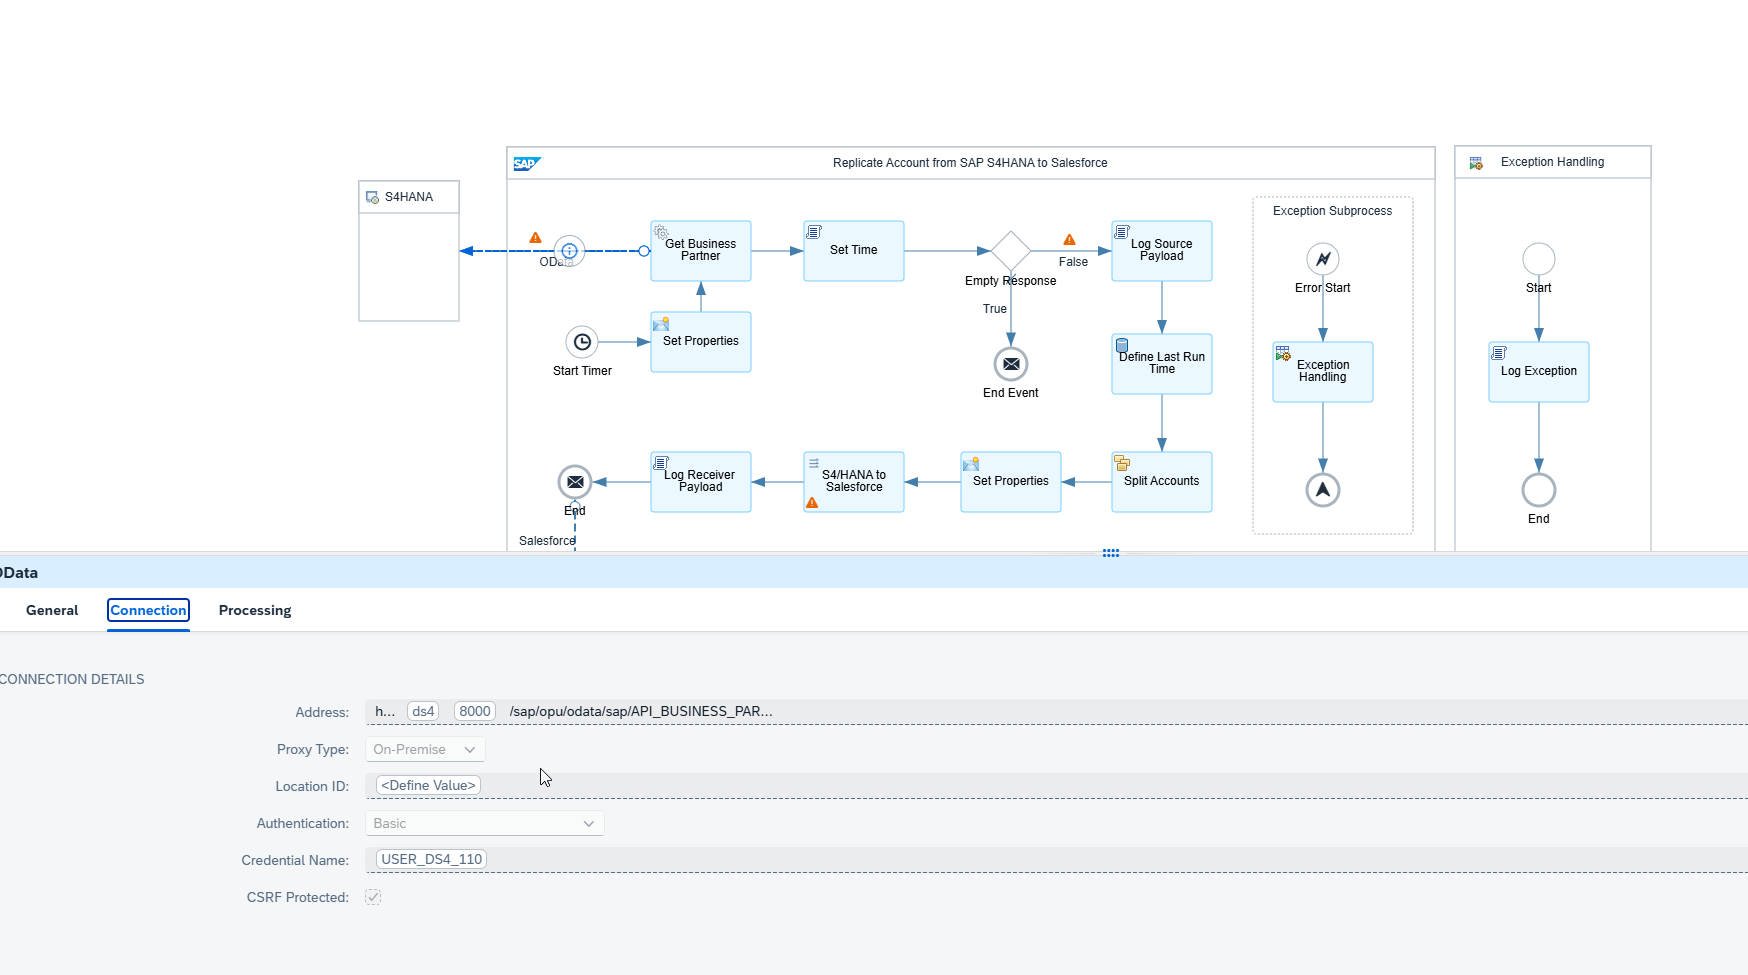
\includegraphics[width=0.95\textwidth]{Appendix/images/GetS4.png}}
    \caption{SAP S/4HANA Endpoint for Fetching Newly Created Business Partners}
    \label{fig:s4_endpoint}
\end{figure}

\noindent This image displays the \textbf{SAP BTP Integration Flow (iFlow)} used to fetch newly created Business Partners (BP) from \textbf{SAP S/4HANA} and replicate them into \textbf{Salesforce}. 

The upper section illustrates the flow's logical steps:
\begin{itemize}
    \item Fetching Business Partner data from SAP S/4HANA.
    \item Setting timestamps to track the last processed record.
    \item Handling exceptions and logging payload details.
\end{itemize}

The lower section highlights the \textbf{Connection Details} of the SAP S/4HANA endpoint:
\begin{itemize}
    \item The \textbf{OData service endpoint} (\texttt{/sap/opu/odata/sap/API\_BUSINESS\_PAR...}) used to retrieve Business Partner data.
    \item \textbf{Proxy Type}: On-Premise, indicating that the connection is routed through an \textbf{SAP Cloud Connector}.
    \item \textbf{Authentication Method}: Basic Authentication for secure access.
    \item \textbf{Credential Name}: The user credentials used to authenticate against the SAP system.
\end{itemize}

This configuration fetches only newly created Business Partners from \textbf{SAP S/4HANA} for synchronization with \textbf{Salesforce}.

\paragraph{}
\textbf{API Query Configuration}

\begin{figure}[h]
    \centering
    \fbox{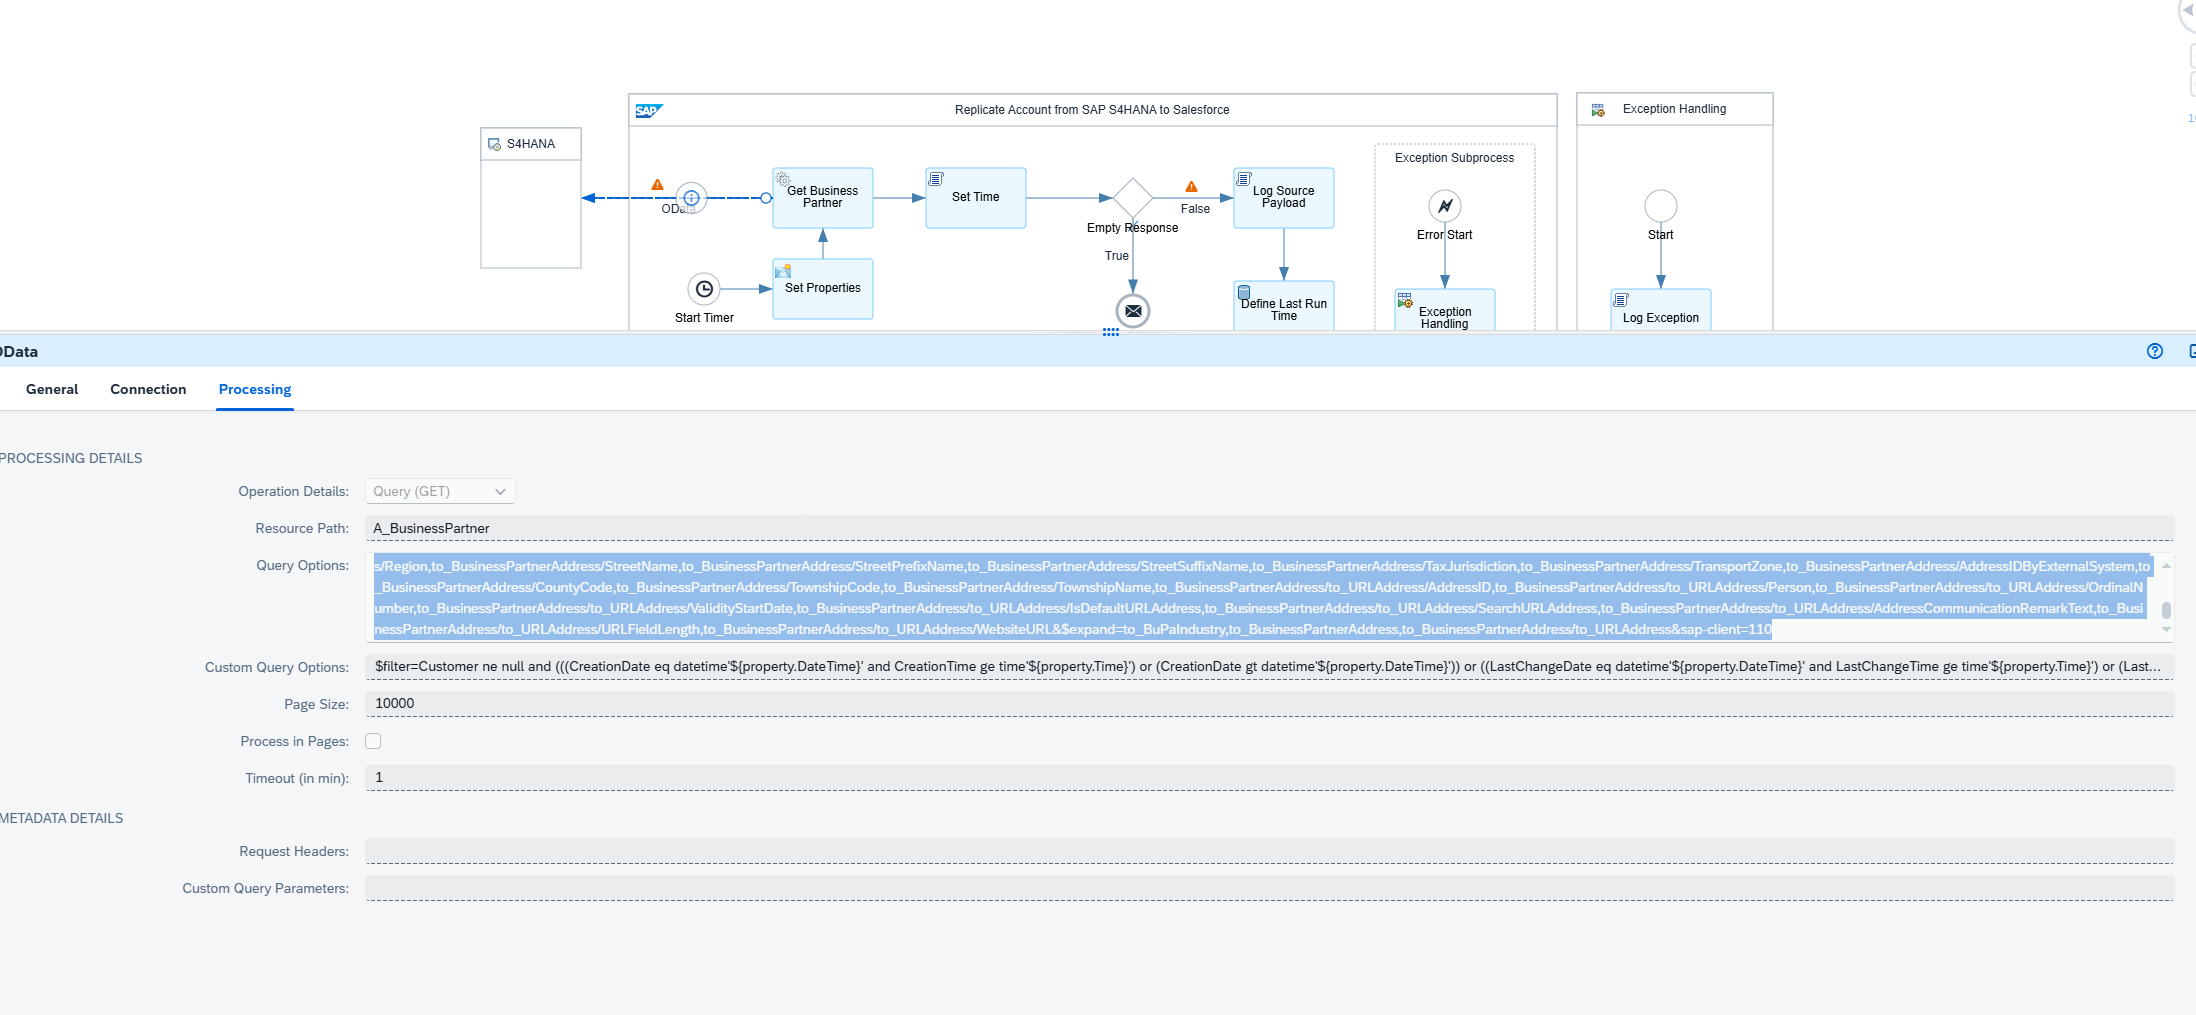
\includegraphics[width=0.95\textwidth]{Appendix/images/QueryS4.png}}
    \caption{API Query Configuration for Fetching All Business Partners in SAP S/4HANA}
    \label{fig:bp_api_query}
\end{figure}

\noindent This image displays the \textbf{SAP BTP Integration Suite's Processing Details} for the \textbf{Business Partner (BP) API query} in SAP S/4HANA. The \textbf{Query (GET) operation} is configured to retrieve \textbf{all Business Partners} using the \texttt{/A\_BusinessPartner} OData service.

Key configurations in the image include:
\begin{itemize}
    \item \textbf{Resource Path}: \texttt{/A\_BusinessPartner}, which fetches Business Partner records from SAP S/4HANA.
    \item \textbf{Query Options (\$select)}: Specifies all relevant fields, including \texttt{BusinessPartner ID}, \texttt{Name}, \texttt{Customer}, \texttt{Supplier}, \texttt{Industry}, \texttt{Address}, and other key attributes. These fields are selected to ensure that all critical information required for mapping and synchronization between SAP S/4HANA and Salesforce is retrieved. For instance, \texttt{BusinessPartner ID} serves as a unique identifier, while fields like \texttt{Name}, \texttt{Customer}, and \texttt{Supplier} provide essential business context. The inclusion of \texttt{Industry} and \texttt{Address} ensures that the integration captures comprehensive details necessary for accurate data representation in Salesforce.
    \item \textbf{Custom Query Options (\$filter)}: The condition \texttt{BusinessPartner ne null} ensures that all valid Business Partners are retrieved.
    \item \textbf{Page Size}: Set to \texttt{10,000} to optimize data retrieval in large batches.
    \item \textbf{Timeout}: Configured to \texttt{1 minute} to prevent long-running queries from failing.
\end{itemize}

This configuration ensures a \textbf{comprehensive data extraction} of all Business Partners from SAP S/4HANA, allowing seamless integration with \textbf{Salesforce} via SAP BTP.


\paragraph{}
\textbf{Salesforce Configuration}

\begin{figure}[h]
    \centering
    \fbox{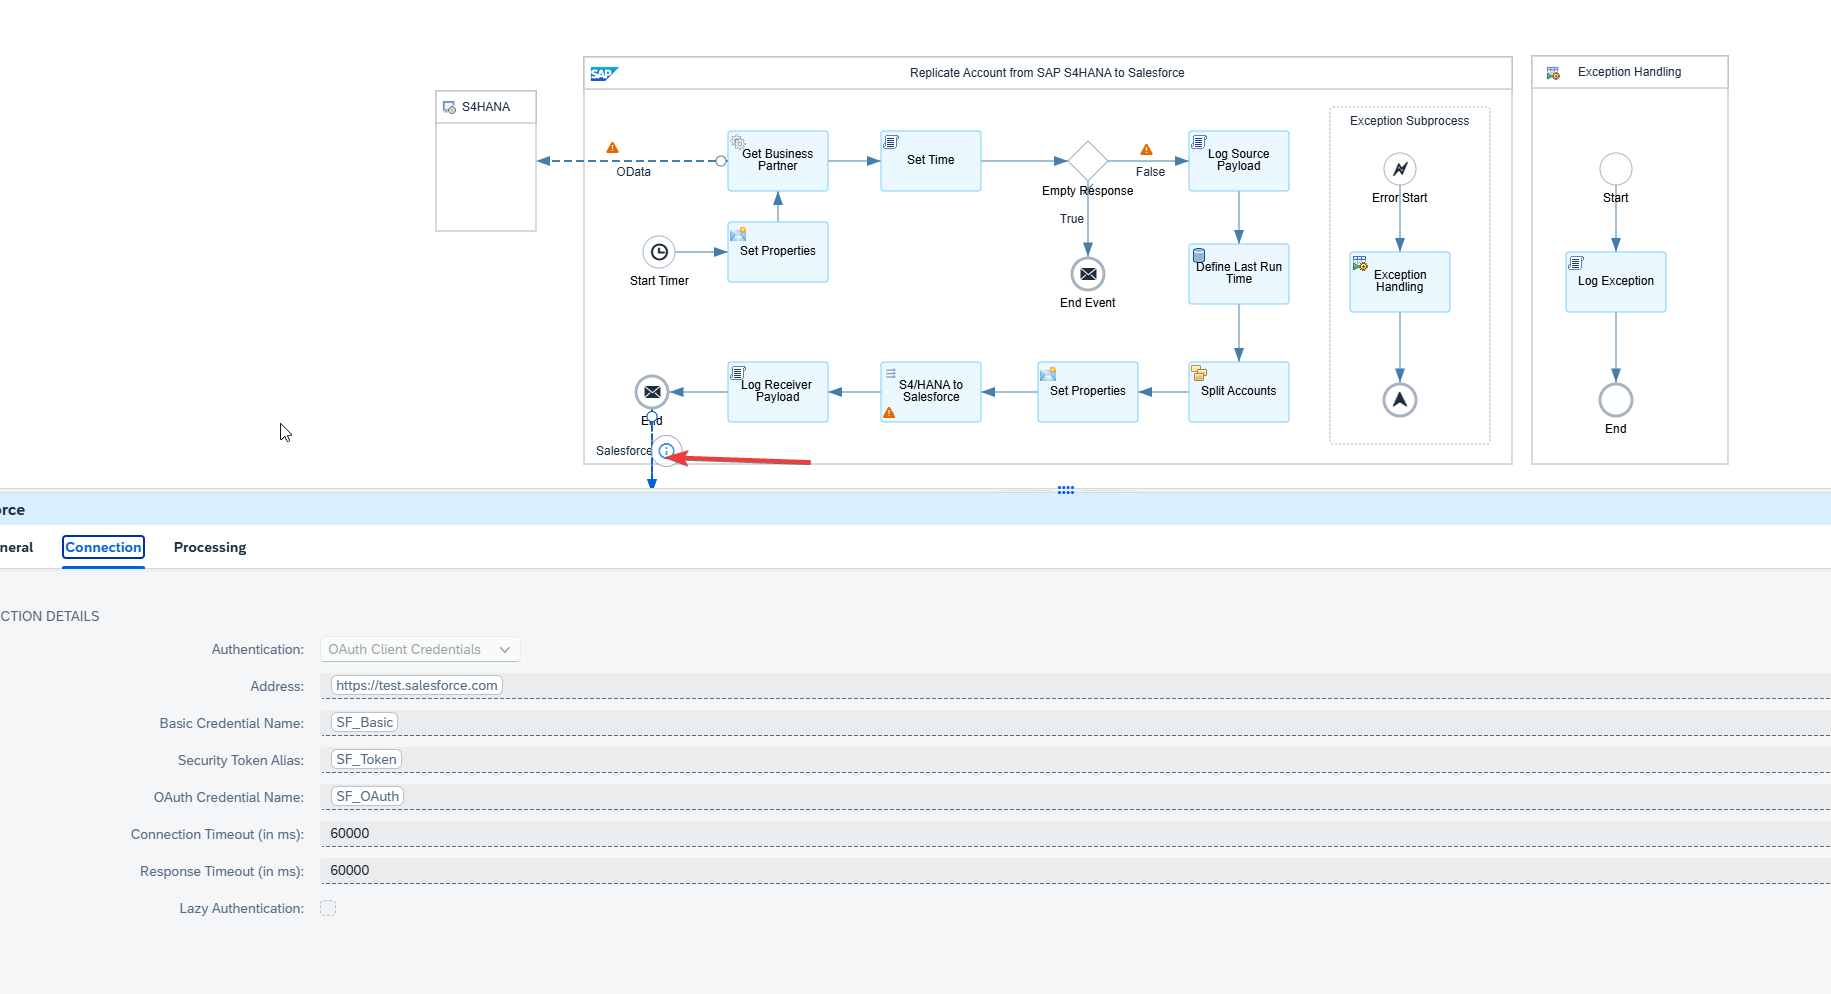
\includegraphics[width=0.95\textwidth]{Appendix/images/SF_Rec.png}}
    \caption{Salesforce Receiver API Configuration in SAP BTP}
    \label{fig:sf_receiver_api}
\end{figure}

\noindent This image displays the \textbf{Salesforce Receiver API Configuration} in the \textbf{SAP BTP Integration Suite}, which is responsible for transferring Business Partner (BP) data from \textbf{SAP S/4HANA} to \textbf{Salesforce}.

Key configurations in the image include:
\begin{itemize}
    \item \textbf{Authentication Method}: OAuth Client Credentials, ensuring secure access to the Salesforce API.
    \item \textbf{Address}: The Salesforce endpoint (\texttt{https://test.salesforce.com}) where Business Partner data is sent.
    \item \textbf{Security Token Alias}: Uses the alias \texttt{SF\_Token} for API authentication.
    \item \textbf{OAuth Credential Name}: \texttt{SF\_OAuth}, which is used for handling token-based authentication.
    \item \textbf{Connection Timeout}: Set to \texttt{60,000 ms} to allow sufficient response time from Salesforce.
    \item \textbf{Response Timeout}: Also set to \texttt{60,000 ms} to handle delays in API response processing.
\end{itemize}


\paragraph{}
\textbf{Salesforce Processing Configuration}

This configuration ensures that data synchronization between SAP S/4HANA and Salesforce is performed securely and efficiently, using OAuth-based authentication for authorization.

\begin{figure}[h]
    \centering
    \fbox{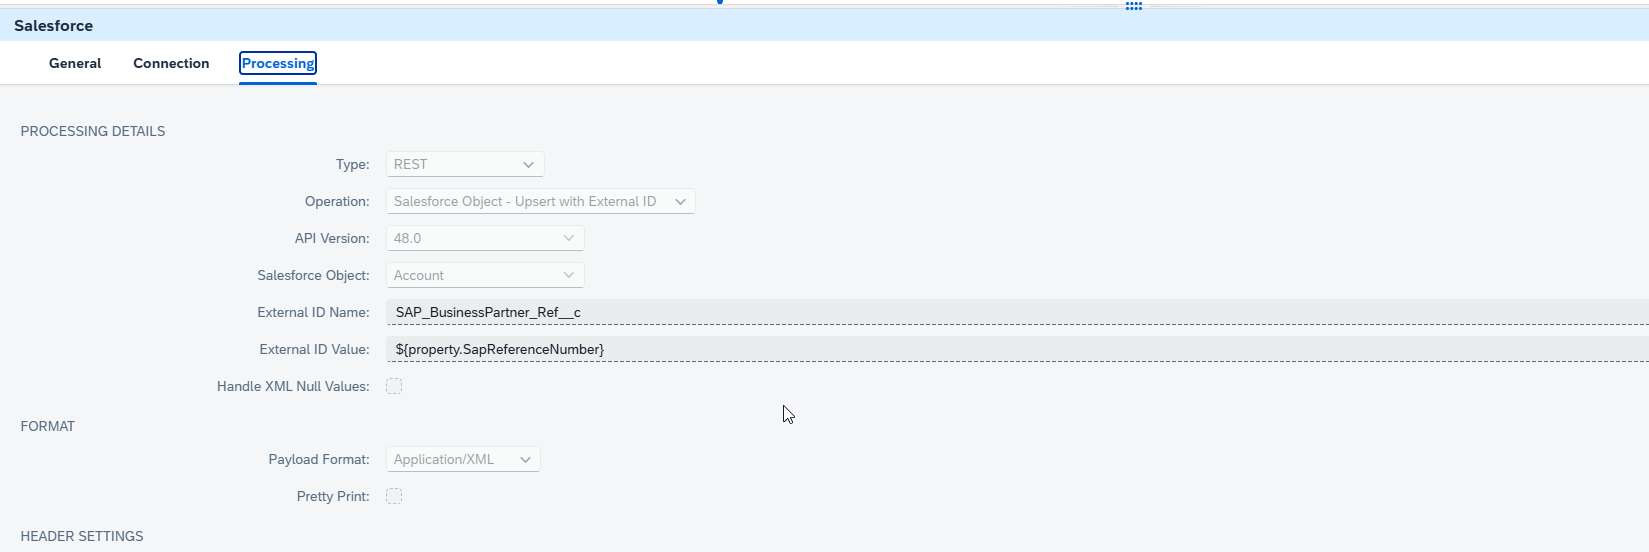
\includegraphics[width=0.95\textwidth]{Appendix/images/SF_API.png}}
    \caption{Salesforce Processing Configuration for Upserting Business Partners}
    \label{fig:sf_processing}
\end{figure}

\noindent This image displays the \textbf{Salesforce Processing Configuration} in the \textbf{SAP BTP Integration Suite}, where Business Partner (BP) data from \textbf{SAP S/4HANA} is upserted into \textbf{Salesforce}.

Key configurations in the image include:
\begin{itemize}
    \item \textbf{Type}: REST API, indicating that data is sent via a web service.
    \item \textbf{Operation}: \texttt{Salesforce Object - Upsert with External ID}, ensuring that records are either updated if they exist or created if they do not.
    \item \textbf{API Version}: \texttt{48.0}, specifying the Salesforce API version used for communication.
    \item \textbf{Salesforce Object}: \texttt{Account}, meaning the data is mapped to the Salesforce Account entity.
    \item \textbf{External ID Name}: \texttt{SAP\_BusinessPartner\_Ref\_\_c}, a custom field used to identify Business Partner records uniquely in Salesforce.
    \item \textbf{External ID Value}: \texttt{\$\{property.SapReferenceNumber\}}, dynamically passing the SAP Business Partner ID to Salesforce for matching records.
    \item \textbf{Payload Format}: \texttt{Application/XML}, specifying that data is transferred in XML format.
\end{itemize}

This configuration ensures that Business Partner records from \textbf{SAP S/4HANA} are **synchronized accurately with Salesforce**, leveraging an **upsert operation** to prevent duplicate records while maintaining data consistency.


\section{Appendix B: Video Demonstration of SAP S/4HANA and Salesforce Integration}

This appendix includes a recorded demonstration of the end-to-end integration process between SAP S/4HANA and Salesforce using SAP BTP Integration Suite. The video showcases data synchronization, API calls, and error handling in real-time.



\noindent This appendix includes video demonstrations of the SAP S/4HANA to Salesforce integration process, highlighting both a failed and a successful attempt.

\bigskip

\noindent\textbf{Failed Attempt: Account Creation to Salesforce}  

\noindent During this attempt, the integration flow encountered an error while transferring an account from SAP S/4HANA to Salesforce. The video demonstrates:
\begin{itemize}
    \item The integration flow execution in SAP BTP Integration Suite.
    \item The error message received during the process.
    \item Debugging steps taken to identify potential causes of failure.
\end{itemize}

\noindent Watch the video using the link below or by scanning the QR code:

\noindent \textbf{URL:} \href{https://drive.google.com/file/d/1qYmTXes5Tejw8vLCC0j5ul4r7GYKo6Hq/view?usp=drive_link}{\textbf{Click here to watch the failure case.}}

\begin{figure}[h]
    \centering
    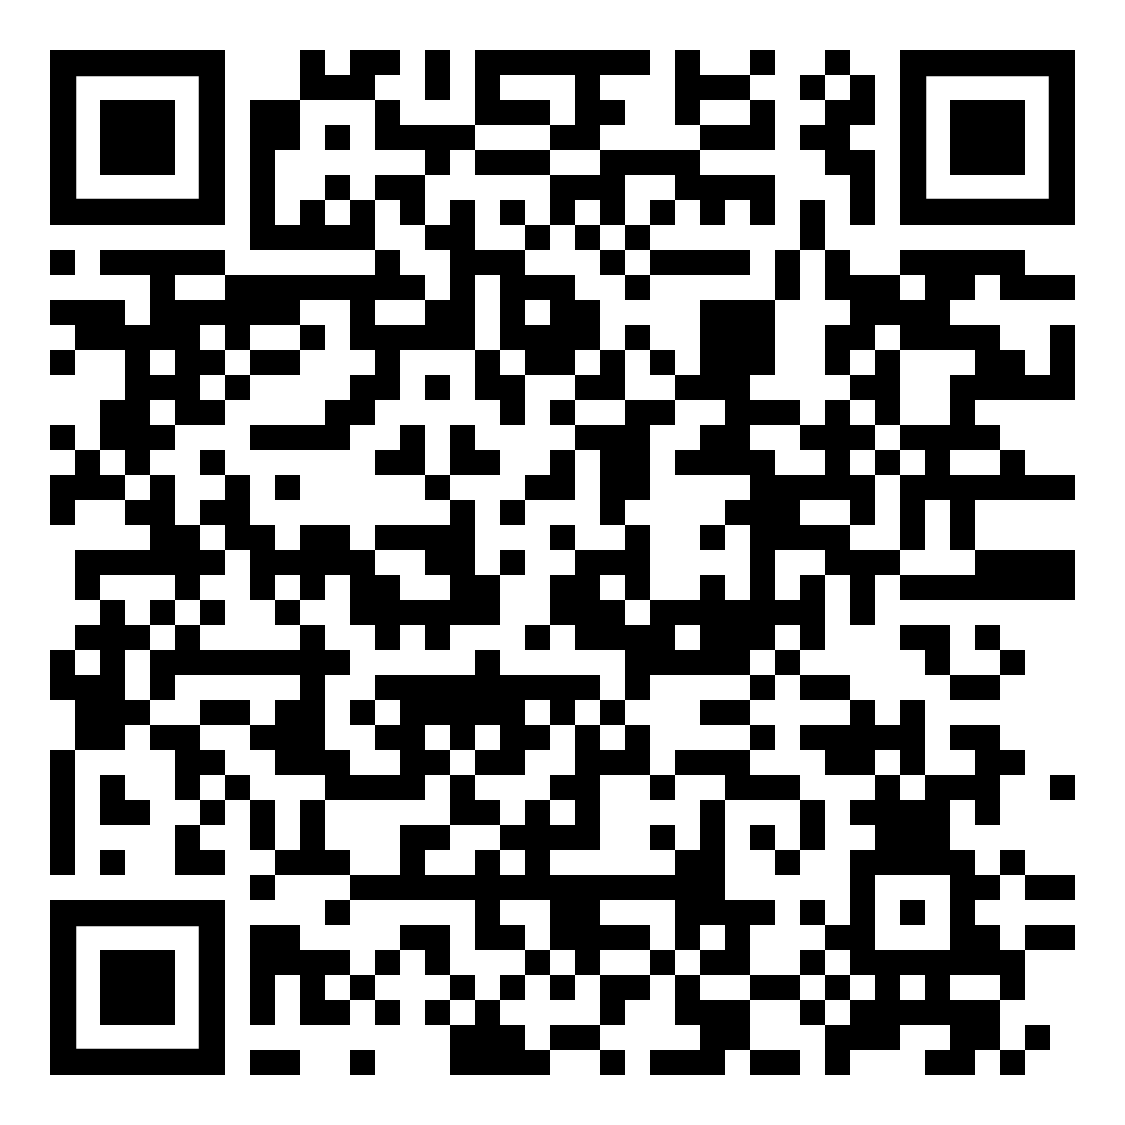
\includegraphics[width=0.3\textwidth]{Appendix/images/Fail_QR.png} % Replace with actual file name
    \caption{Scan to watch: Failed Account Creation to Salesforce}
    \label{fig:failed_video}
\end{figure}

\bigskip

\noindent\textbf{Successful Attempt: Account Creation to Salesforce}  

\noindent This video demonstrates a successful transfer of an account from SAP S/4HANA to Salesforce using the same integration flow, after resolving previous errors. It includes:
\begin{itemize}
    \item Step-by-step execution of the SAP BTP iFlow.
    \item Verification that the account is created in Salesforce without errors.
    \item Key insights into how error handling was improved.
\end{itemize}

\noindent Watch the video using the link below or by scanning the QR code:

\noindent \textbf{URL:} \href{https://drive.google.com/file/d/1YJu7LIanmCPygF6MYpwy4AShSuE6Bh88/view?usp=drive_link}{\textbf{Click here to watch the successful integration.}}

\begin{figure}[h]
    \centering
    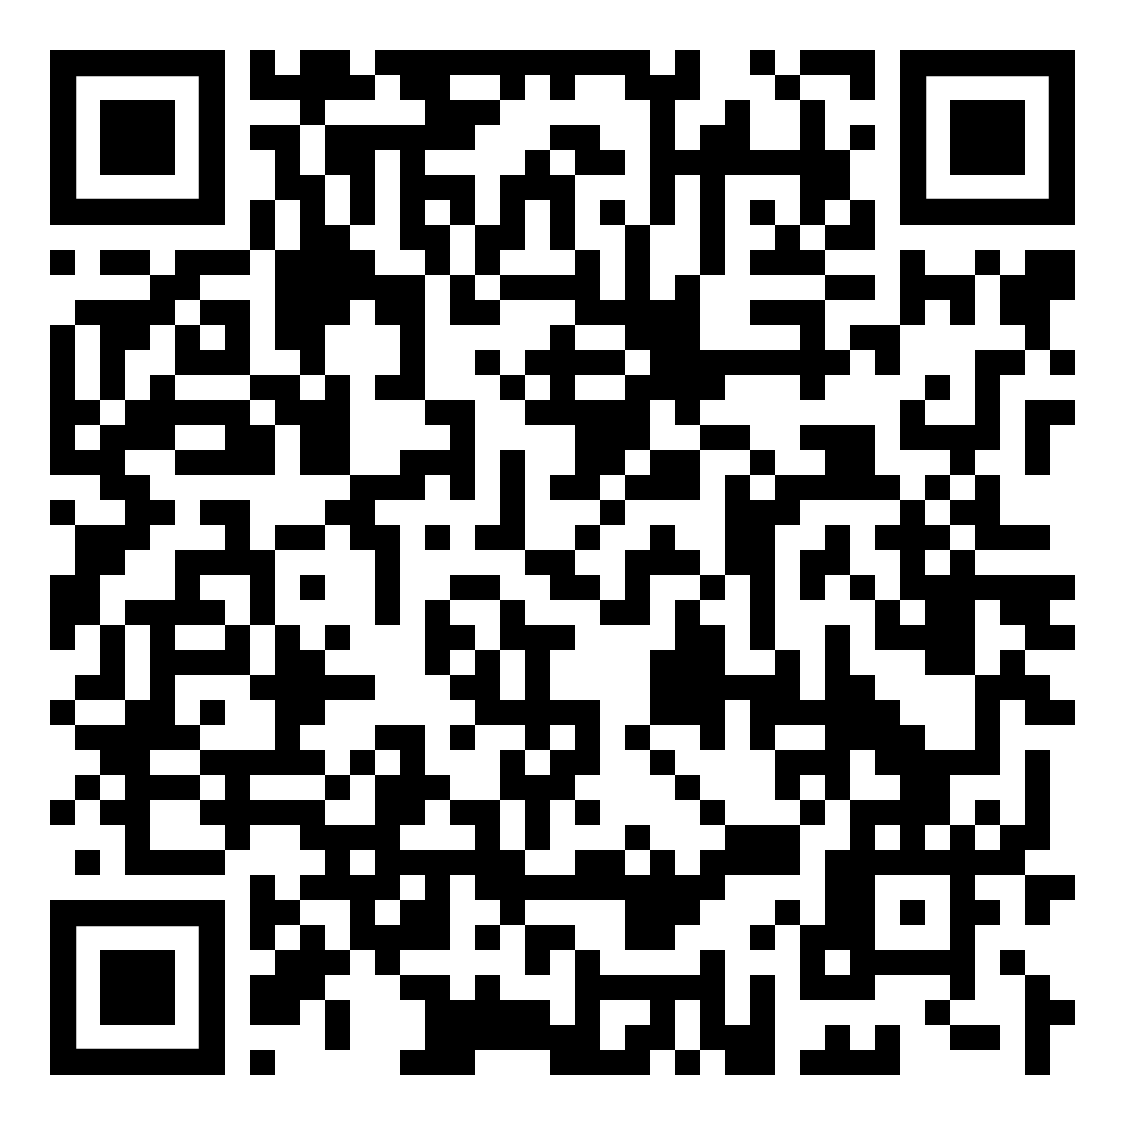
\includegraphics[width=0.3\textwidth]{Appendix/images/Success_QR.png} % Replace with actual file name
    \caption{Scan to watch: Successful Account Creation to Salesforce}
    \label{fig:success_video}
\end{figure}



%=== END OF CHAPTER SIX ===
\newpage

%==== END OF ALL ===
\end{document}
